\documentclass[twoside,spanish,a4paper,12pt]{report}

\usepackage{aeguill,picins,ae,ulem}
\usepackage{geometry}
\geometry{verbose,a4paper,tmargin=2.4cm,bmargin=2.4cm,lmargin=2.4cm,rmargin=2.4cm}
\pagestyle{headings}

\usepackage[spanish]{babel}
\usepackage[T1]{fontenc}
\usepackage[latin1]{inputenc}

\usepackage{array}
\usepackage{bbm}
\usepackage{color}
\usepackage{multirow}

\usepackage{graphicx}

\usepackage{longtable}

\usepackage{makeidx}

\makeindex

\title{\vspace{-1cm}
       
\includegraphics[scale=0.7]{Imagenes/00_Portada/xLogo.png}\\
       \Huge Manual del Usuario\\*[1.0cm]}

\author{\Large Original en Franc\'es: Lo\"ic Le Coq\\*[0.5cm]
        \Large Traducci\'on: \'Alvaro Vald\'es y Marcelo Duschkin\\*[1.0cm]}

\date{\texttt{http://xlogo.tuxfamily.org} %\Large Actualizado: \today}
\begin{center}
   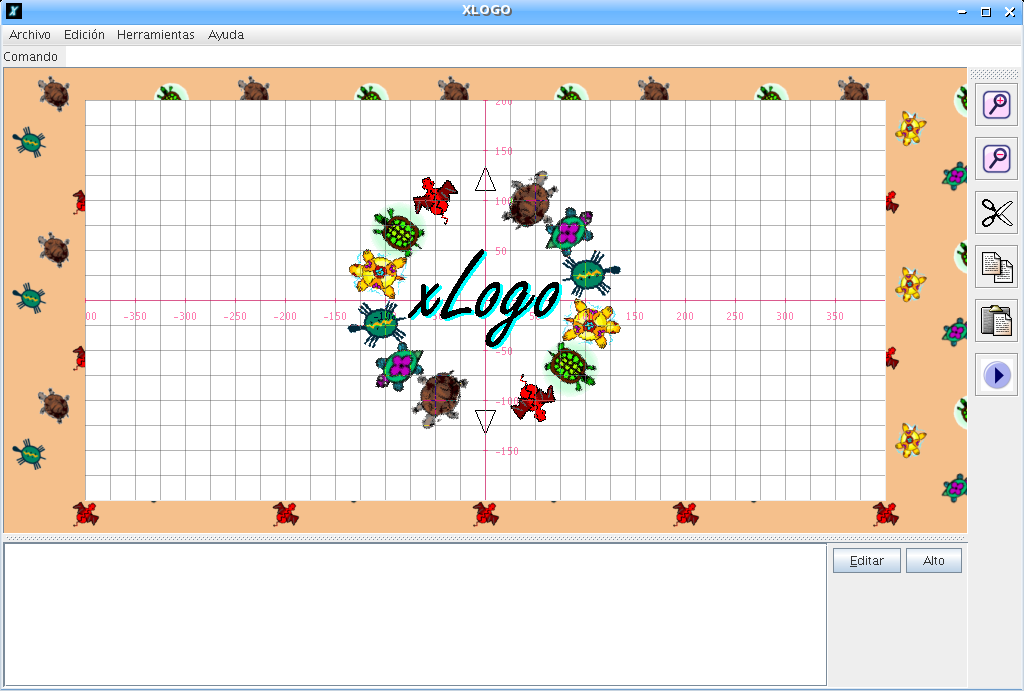
\includegraphics[scale=0.4]{Imagenes/00_Portada/Portada_es_091.png}
\end{center}
}

\begin{document}

\maketitle

\tableofcontents

\chapter{Presentaci\'on}
   \label{Presentacion}

\section{Introducci\'on}
   \label{Introduccion}

\textsc{Logo} es un lenguaje desarrollado a finales de los a\~nos 60 por
Seymour Papert. Es un lenguaje excelente para comenzar a estudiar
programaci\'on, y ense\~na lo b\'asico acerca de temas como bucles,
condicionales, procedimientos, etc. El usuario puede mover un objeto llamado 
``tortuga'' dentro de la pantalla, usando instrucciones (comandos) simples
como ``\texttt{avanza}'', ``\texttt{retrocede}'', ``\texttt{giraderecha}''
y similares. Con cada movimiento, la tortuga deja un ``rastro'' (dibuja
una l\'inea) tras de s\'i, y de esta manera se crean gr\'aficos. Tambi\'en
es posible operar con palabras y listas.\\

Este estilo gr\'afico hace de \textsc{Logo} un lenguaje ideal para
principiantes, y especialmente f\'acil para los ni\~nos. \\

\textsc{\textbf{XLogo}} es un int\'erprete \textsc{Logo} escrito en
\textsc{Java}. Actualmente soporta diez idiomas (Franc\'es, Ingl\'es,
Espa\~nol, Portugu\'es, \'Arabe, Esperanto, Gallego, Asturiano y Griego) y se
distribuye bajo licencia GPL. Por lo tanto, este programa es libre en cuanto
a libertad y gratuidad.

\section{Java}
   \label{Java}

Como hemos mencionado, \textsc{XLogo} est\'a escrito en \textsc{Java}.
\textsc{Java} es un lenguaje que tiene la ventaja de ser multi-plataforma; esto
es, \textsc{XLogo} podr\'a ejecutarse en cualquier sistema operativo que soporte
\textsc{Java}; tanto usando Linux como Windows, MacOS o Solaris, \textsc{XLogo}
funcionar\'a sin problemas.

\chapter{Caracter\'isticas de la Interfaz}
   \label{Caracteristicas_Interfaz}

\section{Primera Ejecuci\'on}
   \label{Primera_Ejecucion}

La primera vez que ejecute \textsc{XLogo} (o si ha borrado el fichero
\texttt{.xlogo} -- ver secci\'on \ref{Desinstalar}) deber\'a elegir
el idioma con que quiere trabajar, seleccionando la bandera correspondiente
y haciendo \textit{click} en el bot\'on \texttt{OK}.
\begin{center}
   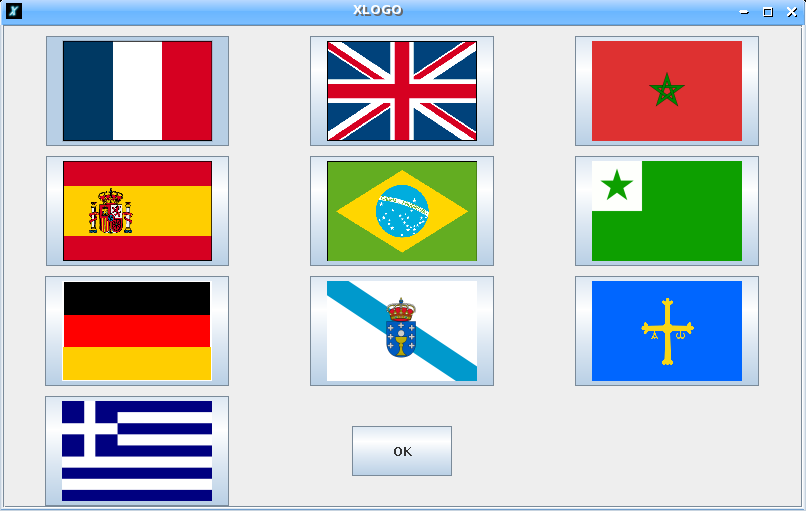
\includegraphics[scale=0.2]{Imagenes/02_Caracteristicas/PantallaIdioma.png}
\end{center}
Esta elecci\'on no es definitiva; puede elegir otro idioma en cualquier
momento desde las opciones de men\'u (secci\'on \ref{Menu-Herramientas})

\section{La ventana principal}
   \label{La-ventana-principal}

\begin{center}
   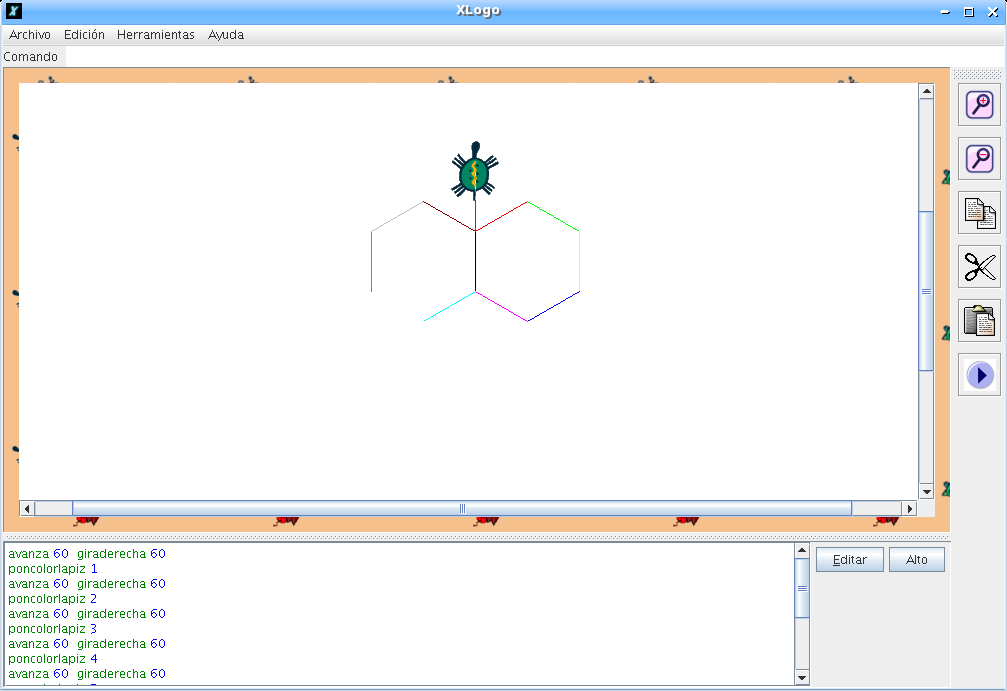
\includegraphics[scale=0.35]{Imagenes/02_Caracteristicas/VentanaPcpal_090.png}
\end{center}

\begin{itemize}
   \item En la fila superior, est\'an las entradas t\'ipicas de men\'u:
      \textbf{Archivo}, \textbf{Edici\'on}, \textbf{Herramientas},
      \textbf{Ayuda}
   \item Justo debajo est\'a la 
      \textbf{L\'inea de Comando},\index{L\'inea de Comando}
      donde se escriben las instrucciones \textsc{Logo}.
   \item En el medio de la pantalla, est\'a el
      \textbf{\'Area de Dibujo} \index{Area@\'Area de Dibujo}
      (donde se mueve la tortuga).
   \item A la derecha del \'area de dibujo se encuentra una barra de
      herramientas vertical con las funciones \textit{zoom}\index{Zoom}
      (acercar y alejar), \textit{copiar},\index{Copiar}
      \textit{cortar}\index{Cortar}, \textit{pegar}\index{Pegar} y
      \textit{Comando de Inicio}\index{Comando de Inicio}.
   \item Al pie, est\'a la ventana del
      \textbf{Hist\'orico de Comandos},\index{Hist\'orico de Comandos}
      que muestra todo lo ingresado y sus respuestas asociadas. Para
      reutilizar un comando previamente ingresado, hay dos opciones:
      Hacer un \textit{click} en un comando del hist\'orico, o usar
      las teclas de flecha arriba y flecha abajo del teclado (lo que
      es m\'as pr\'actico).
   \item A la derecha de la ventana del hist\'orico hay dos botones:
      \textbf{Editar} y \textbf{Alto}. 
      \begin{itemize}
         \item \textbf{Editar} \index{Editar} permite abrir la ventana del
            editor de procedimientos. 
         \item \textbf{Alto} \index{Alto} interrumpe la ejecuci\'on del
            programa ingresado.
      \end{itemize}
\end{itemize}

\section{El editor de procedimientos}
   \label{EditorProcedimientos}
   \index{Editor de Procedimientos}

\begin{center}
   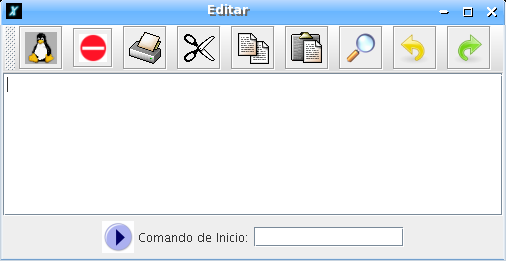
\includegraphics[scale=0.5]
      {Imagenes/02_Caracteristicas/EditorProc_092.png}
\end{center}

Hay cuatro maneras de abrir el editor:
\begin{itemize}
   \item Escribir \texttt{editatodo}\index{editatodo@\texttt{editatodo}} o
      \texttt{edtodo}\index{edtodo@\texttt{edtodo}} en la
      \textbf{L\'inea de Comando}. La ventana del editor se abrir\'a
      mostrando todos los procedimientos definidos hasta ese momento.
   \item Si deseas editar un procedimiento en especial (o algunos), debes
      usar \texttt{ed}\index{ed@\texttt{ed}} o \texttt{edita}\index{edita@\texttt{edita}}
      en la l\'inea de comandos seguido del nombre de procedimiento, o la lista con los
      nombres de procedimientos que deseas editar: \\
      \texttt{edita \char`\"{}nombre\_procedimiento} \\
      o: \\
      \texttt{edita [proc\_1 proc\_2]}
   \item Hacer \textit{click} en el bot\'on \textbf{Editar}.
      \index{Editar}
   \item Usar el atajo de teclado \texttt{Alt+E}
\end{itemize}
Estos son los diferentes botones que encontrar\'as en la ventana del
Editor:
\begin{center} \begin{longtable}{|m{1.3cm}|m{115mm}|} \hline 
   \includegraphics[scale=1.0]{Imagenes/02_Caracteristicas/guardar.png} &
      Guarda en memoria los cambios hechos en el editor y cierra la ventana.
      Es este bot\'on el que se debe usar cada vez que quieras aplicar los
      procedimientos recientemente incorporados.

      Atajo de teclado: \texttt{ALT+Q}. \\ \hline 
   
\includegraphics[scale=1.0]{Imagenes/02_Caracteristicas/salir.png} &
      Cierra la ventana del editor sin guardar los \'ultimos cambios. Ten
      presente que NO aparece ning\'un mensaje de confirmaci\'on. Aseg\'urate
      bien de que realmente no hay nada que guardar.

      Atajo de teclado: \texttt{ALT+C}. \\ \hline 
   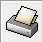
\includegraphics[scale=1.0]{Imagenes/02_Caracteristicas/imprimir.png} & 
      Imprime el contenido del editor.\\ \hline 
   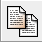
\includegraphics[scale=1.0]{Imagenes/02_Caracteristicas/copiar.png} &
      Copia el texto seleccionado al portapapeles.

      Atajo de teclado: \texttt{Control+C}.\\ \hline 
   
\includegraphics[scale=1.0]{Imagenes/02_Caracteristicas/cortar.png} &
      Corta el texto seleccionado y lo copia al portapapeles.

      Atajo de teclado: \texttt{Control+X}.\\ \hline 
   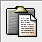
\includegraphics[scale=1.0]{Imagenes/02_Caracteristicas/pegar.png}&
      Pega el contenido del portapapeles.

      Atajo de teclado: \texttt{Control+V}.\\ \hline
   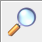
\includegraphics[scale=1.0]{Imagenes/02_Caracteristicas/lupa.png}&
      Permite realizar b\'usquedas y reemplazos en los procedimientos. Para
      ello se abre la ventana siguiente:
      \begin{center}
         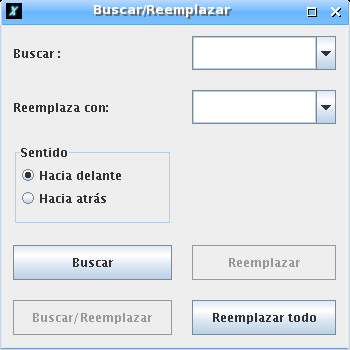
\includegraphics[scale=0.45]{Imagenes/02_Caracteristicas/BuscarReemplazar.png}
      \end{center} \\ \hline
   
\includegraphics[scale=1.0]{Imagenes/02_Caracteristicas/undo.png}&
      Permite deshacer los \'ultimos cambios realizados en los procedimientos.\\ \hline
   
\includegraphics[scale=1.0]{Imagenes/02_Caracteristicas/redo.png}&
      ``Rehace'' lo deshecho con el bot\'on anterior.\\ \hline
\end{longtable} \end{center}

\textbf{Nota:} Aunque aqu\'i se representa la imagen de Tux (mascota de Linux) en el
bot\'on ``\textit{Guardar}'', en realidad se muestra la tortuga activa para dar la
idea de ``\textit{enviar la informaci\'on a la tortuga}''; por ejemplo, si la tortuga
activa es la n\'umero 3 (secci\'on \ref{Menu_Preferencias}):
\begin{center}
   \includegraphics[scale=0.5]{Imagenes/02_Caracteristicas/EditorProc_093.png}
\end{center}

En la parte inferior se encuentra l\'inea donde definir el
\texttt{Comando de Inicio}, que se activa con el bot\'on situado a la derecha
del \'Area de Dibujo.
\begin{center}
   
\includegraphics[scale=0.5]{Imagenes/02_Caracteristicas/Boton_Inicio.png}
\end{center}
Al pulsar el bot\'on, se ejecuta inmediatamente el \texttt{Comando de Inicio}
sin necesidad de escribirlo en la L\'inea de Comandos, lo que es \'util para:
\begin{itemize}
   \item Ahorrar tiempo mientras se desarrolla un programa
   \item Al enviar un programa a alguien que se inicia en \textsc{Logo}, simplemente
      tiene que hacer ``\textit{click}'' en ese bot\'on para ejecutarlo
   \item \ldots \\
\end{itemize}

\noindent \textbf{IMPORTANTE}:
\begin{itemize}
   \item Nota que hacer \textit{click} en el icono de cierre 
      (
\includegraphics[scale=0.4]{Imagenes/02_Caracteristicas/cerrar.png}) %\texttt{[x]} de la
      de la barra de t\'itulo de la ventana del Editor, no hace nada. Solamente
      funcionan los dos botones principales.
   \item Para borrar los procedimientos que no se necesitan, usa los comandos
      \texttt{borra} \index{borra@\texttt{borra}} y 
      \texttt{borratodo} \index{borratodo@\texttt{borratodo}} o en la barra
      de men\'us: Herramientas $\rightarrow$ Borra procedimientos.
      \index{Borrar procedimientos}
\end{itemize}
Al hacer \textit{click} para imprimir, aparecer\'a una ventana de di\'alogo
donde podremos configurar distintas opciones de impresi\'on:
\begin{itemize}
   \item \textbf{General}: Impresora a utilizar, Imprimir a un archivo, Rango
      de Impresi\'on y N\'umero de copias.
      \begin{center}
         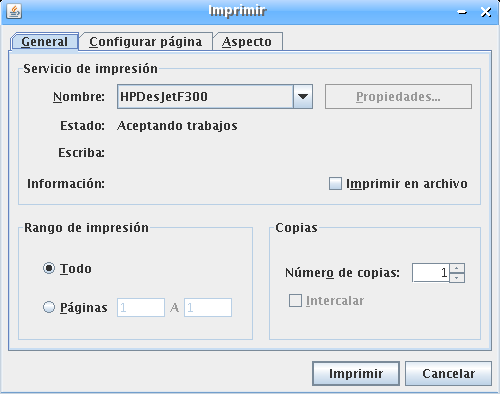
\includegraphics[scale=0.3]{Imagenes/02_Caracteristicas/VentanaImpresion_01.png}
      \end{center}
   \item \textbf{Configurar P\'agina}: Tipo de papel, Origen del papel,
      Orientaci\'on de la Hoja y M\'argenes
      \begin{center}
         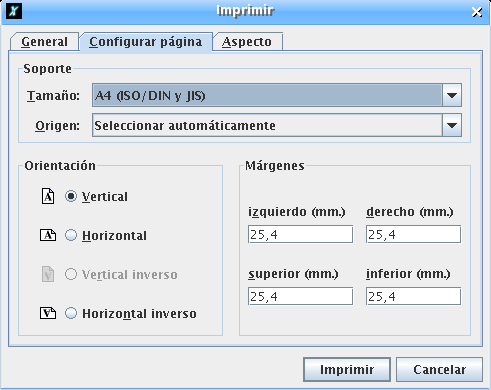
\includegraphics[scale=0.3]{Imagenes/02_Caracteristicas/VentanaImpresion_02.png}
      \end{center}
   \item \textbf{Aspecto}: Color (cuando disponible), Calidad, Caras y otros
      Atributos 
      \begin{center}
         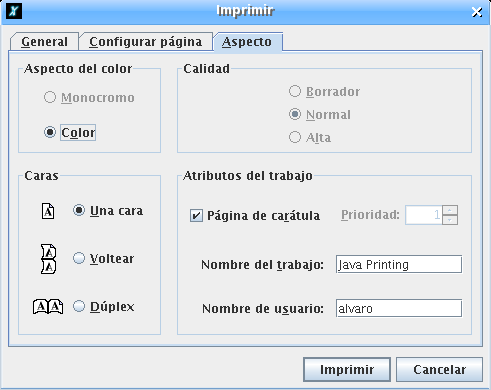
\includegraphics[scale=0.3]{Imagenes/02_Caracteristicas/VentanaImpresion_03.png}
      \end{center}
\end{itemize}

\section{Salir}
   \label{Salir}
   \index{Salir}

Para salir simplemente seleccionamos: \textbf{Archivo} $\rightarrow$ \textbf{Salir},
o hacemos \textit{click} en en el icono de cierre 
(
\includegraphics[scale=0.4]{Imagenes/02_Caracteristicas/cerrar.png}). \textsc{XLogo} presentar\'a
una ventana de confirmaci\'on: 
\begin{center}
   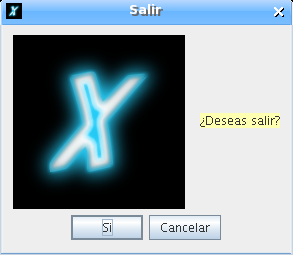
\includegraphics[scale=0.4]{Imagenes/02_Caracteristicas/SalirXLogo.png}
\end{center}
Pulsamos \texttt{S\'i} y termina la ejecuci\'on.


\chapter{Opciones del Men\'u}
   \label{Opciones-del-Menu}

\section{Men\'u ``\textit{Archivo}''}
   \label{Menu-Archivo}

\begin{itemize}
   \item \textbf{Archivo $\rightarrow$ Nuevo}:\index{Nuevo} Elimina todos los
      procedimientos y variables definidos hasta el momento para comenzar un
      nuevo espacio de trabajo. Se abrir\'a una ventana para confirmar la
      eliminaci\'on de todos los procedimeintos y variables:
      \begin{center}
         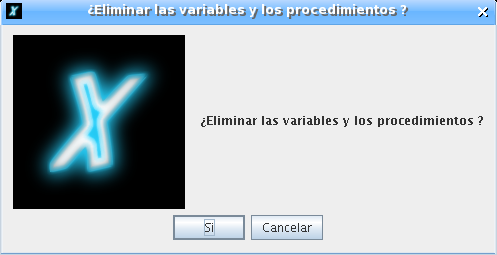
\includegraphics[scale=0.3]{Imagenes/03_Opciones-Menu/MenuNuevo.png}
      \end{center}
   \item \textbf{Archivo $\rightarrow$ Abrir}:\index{Abrir} Carga un archivo
      \textsc{Logo} previamente guardado en disco.
      \begin{center}
         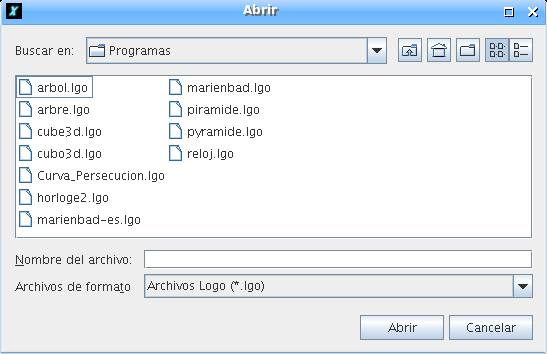
\includegraphics[scale=0.3]{Imagenes/03_Opciones-Menu/MenuAbrir.png}
      \end{center}
   \item \textbf{Archivo $\rightarrow$ Guardar como\ldots{}}:\index{Guardar como ...}
      Graba un archivo (\texttt{.lgo}) de procedimientos definidos hasta ese
      momento en el disco, permitiendo asignarle un nombre. 
      \begin{center}
         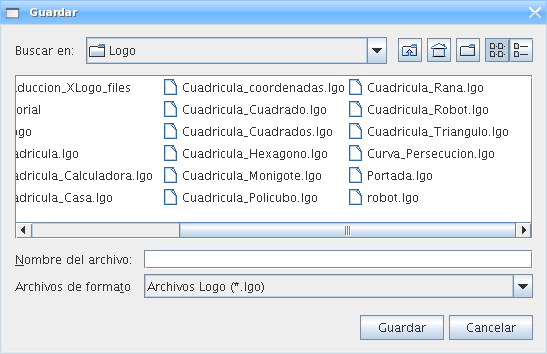
\includegraphics[scale=0.3]{Imagenes/03_Opciones-Menu/MenuGuardar.png}
      \end{center}
   \item \textbf{Archivo $\rightarrow$ Guardar}:\index{Guardar} Graba un archivo
      (\texttt{.lgo}) con los procedimientos definidos hasta ese momento
      en el disco. Esta opci\'on estar\'a deshabilitada mientras no se le haya
      asignado un nombre como se acaba de explicar en el punto anterior.
   \item \textbf{Archivo $\rightarrow$ Capturar imagen $\rightarrow$ Guardar imagen
      como\ldots{}}:\index{Guardar imagen como\ldots} Permite guardar la imagen del
      \'area de dibujo en formato jpg\index{jpg@\texttt{.jpg}} o png.
      \index{png@\texttt{.png}}Para ello, puedes seleccionar previamente una parte
      de la imagen pulsando el bot\'on izquierdo del rat\'on y arrastrando. 
   \item \textbf{Archivo $\rightarrow$ Capturar imagen $\rightarrow$ Imprimir
      imagen}:\index{Imprimir imagen} Permite imprimir la imagen del \'area de
      dibujo. Se puede seleccionar una zona a imprimir tal como se
      explic\'o para \textbf{Guardar}.
   \item \textbf{Archivo $\rightarrow$ Capturar imagen $\rightarrow$ Copiar al
      portapapeles:} \index{Portapapeles} Permite enviar la imagen al portapapeles
      del sistema. Del mismo modo que para \textbf{Imprimir} y \textbf{Guardar},
      se puede seleccionar una zona. Esta opci\'on funciona perfectamente en
      entornos Windows y Mac:
      \begin{center}
         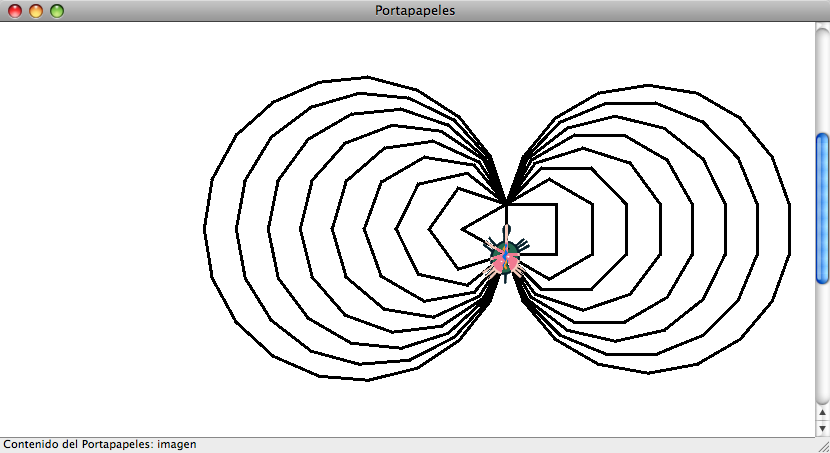
\includegraphics[scale=0.3]{Imagenes/03_Opciones-Menu/Portapapeles_Mac.png}
      \end{center}
      pero no as\'i en entornos Linux (el portapapeles no tiene el mismo
      funcionamiento).
   \item \textbf{Archivo $\rightarrow$ Zona de texto $\rightarrow$ Guardar en
      formato RTF}:\index{Guardar en formato RTF} Guarda el contenido del
      \textbf{Hist\'orico de Comandos} en un fichero con formato RTF \index{RTF}
      (\textit{Rich Text Format}), manteniendo los colores de los mensajes. Si
      no se escribe la extensi\'on \texttt{.rtf}, se a\~nade autom\'aticamente. 
      \begin{center}
         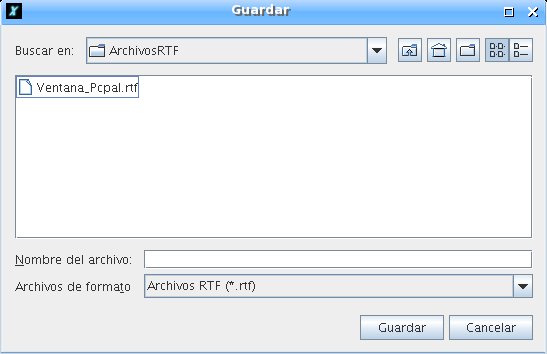
\includegraphics[scale=0.3]{Imagenes/03_Opciones-Menu/Guardar_RTF.png}
      \end{center}
   \item \textbf{Archivo $\rightarrow$ Salir}: \index{Salir} Finaliza la ejecuci\'on
      de \textsc{XLogo}. Tambi\'en puede terminarse la ejecuci\'on desde la L\'inea
      de comandos con la primitiva \texttt{adi\'os}. \index{adi\'os@\texttt{adi\'os}}
\end{itemize}

\section{Men\'u ``\textit{Edici\'on}''}
   \label{Menu-Edicion}
   \index{Edici\'on}

\begin{itemize}
   \item \textbf{Edici\'on $\rightarrow$ Copiar}:\index{Copiar} copia el texto
      seleccionado en el portapapeles. Atajo de teclado: \texttt{Control+C}
   \item \textbf{Edici\'on $\rightarrow$ Cortar}:\index{Cortar} corta el texto
      seleccionado y lo copia en el portapapeles. Atajo de teclado:
      \texttt{Control+X}
   \item \textbf{Edici\'on $\rightarrow$ Pegar}:\index{Pegar} pega el texto desde el
      portapapeles a la l\'inea de comandos. Atajo de teclado:
      \texttt{Control+V}
   \item \textbf{Edici\'on $\rightarrow$ Seleccionar todo}:\index{Seleccionar todo}
      Selecciona todo lo que se encuentra escrito en la
      \textbf{L\'inea de Comandos}.
\end{itemize}

\section{Men\'u ``\textit{Herramientas}''}
   \label{Menu-Herramientas}

\begin{itemize}
   \item \textbf{Herramientas $\rightarrow$ Elegir el color del l\'apiz}:
      \index{Elegir color del l\'apiz} Permite elegir el color con que la
      tortuga dibujar\'a, desde la paleta de colores, mediante una
      definici\'on \texttt{HSB} (\textit{Hue}, \textit{Saturation}, 
      \textit{Brightness} - Tonalidad, Saturaci\'on, Brillo) o desde
      una codificaci\'on \texttt{RVA} (Rojo, Verde y Azul).
      \begin{center}
         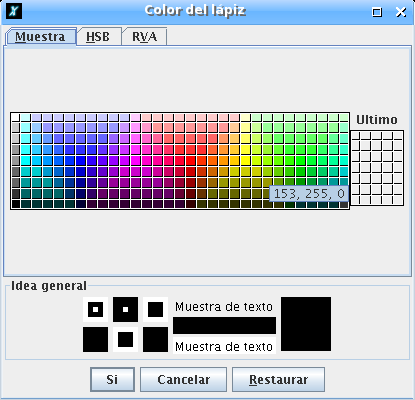
\includegraphics[scale=0.3]{Imagenes/03_Opciones-Menu/ColorLapiz_01.png}
         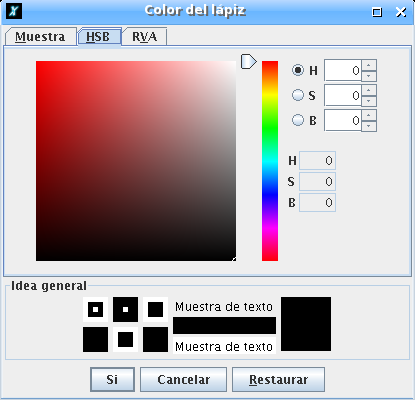
\includegraphics[scale=0.3]{Imagenes/03_Opciones-Menu/ColorLapiz_02.png}
         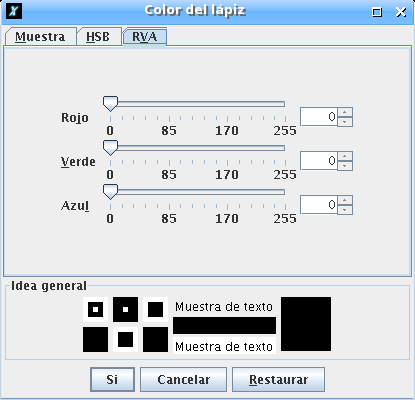
\includegraphics[scale=0.3]{Imagenes/03_Opciones-Menu/ColorLapiz_03.png}
      \end{center}
      Tambi\'en accesible con el comando \texttt{poncolorlapiz}.
      \index{poncolorlapiz@\texttt{poncolorlapiz}} (Secci\'on
      \ref{Propiedades-Tortuga})
   \item \textbf{Herramientas $\rightarrow$ Elegir el color de fondo (papel)}:
      \index{Elegir color del papel} Pone un color como fondo de pantalla,
      con las mismas caracter\'isticas que \textbf{Elegir Color del L\'apiz}.
      Tambi\'en accesible con el comando \texttt{poncolorpapel}.
      \index{poncolorpapel@\texttt{poncolorpapel}} (Secci\'on
      \ref{Propiedades-Tortuga})
   \item \textbf{Herramientas $\rightarrow$ Definir archivos de inicio}:
      \index{Definir archivos de inicio} Permite establecer la ruta a los
      archivos de inicio.
      \begin{center}
         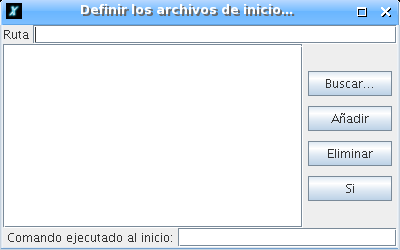
\includegraphics[scale=0.3]{Imagenes/03_Opciones-Menu/DefinirArchivosInicio.png}
      \end{center}
      Cualquier procedimiento contenido en estos archivos
      \texttt{.lgo} \index{lgo@\texttt{.lgo}}
      se convertir\'an en ``\textit{seudo-primitivas}'' del
      lenguaje \textsc{XLogo}. Pero no pueden ser modificadas por el usuario.
      As\'i se pueden definir primitivas personalizadas
      \index{Primitivas personalizadas}.
   \item \textbf{Herramientas $\rightarrow$ Traducir procedimientos}:
      \index{Traducir procedimientos} Abre una caja de di\'alogo que permite
      traducir los comandos \textsc{XLogo} entre dos idiomas. Es muy \'util,
      en particular, cuando se obtienen c\'odigos \textsc{Logo} en ingl\'es
      (de internet, por ejemplo) para expresarlos en el idioma deseado
      (Espa\~nol, Franc\'es, \ldots{})
      \begin{center}
         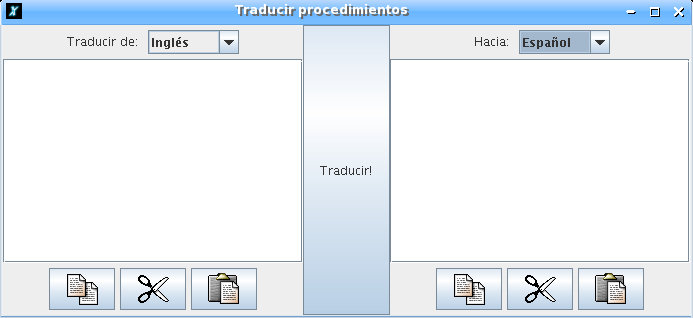
\includegraphics[scale=0.3]{Imagenes/03_Opciones-Menu/TraducirProcedimientos.png}
      \end{center}
   \item \textbf{Herramientas $\rightarrow$ Borra procedimientos}:
      \index{Borrar procedimientos} Abre una caja de di\'alogo que permite
      selccionar el procedimiento que se desea borrar, de una forma m\'as
      sencilla que con la primitiva \texttt{borra}.
      \begin{center}
         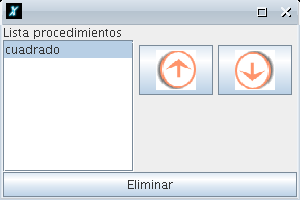
\includegraphics[scale=0.3]{Imagenes/03_Opciones-Menu/BorraProcedimientos.png}
      \end{center}
   \item \textbf{Herramientas $\rightarrow$ Preferencias}:\label{Menu_Preferencias}
      \index{Preferencias}Abre una caja de di\'alogo donde se pueden
      configurar varios aspectos:
      \begin{itemize}
         \item \textbf{General:}
            \begin{itemize}
               \item \textbf{Idioma}: \index{Idioma} Permite elegir entre
                  Franc\'es, Ingl\'es, Espa\~nol, Gal\'es, Portugu\'es,
                  Esperanto, \'Arabe y Gallego. Nota que las primitivas
                  se adec\'uan a cada lenguaje.
               \item \textbf{Aspecto}: \index{Aspecto} Permite definir el
                  aspecto de la ventana \textsc{XLogo}. Est\'an disponibles los
                  estilos ``Windows'', ``Metal'' y ``Motif''.
               \item \textbf{Velocidad de la tortuga}:
                  \index{Velocidad de la tortuga} Si prefieres ver todos
                  los movimientos de la tortuga, puedes reducir la velocidad
                  con la barra deslizante. 
            \end{itemize}
            \begin{center}
               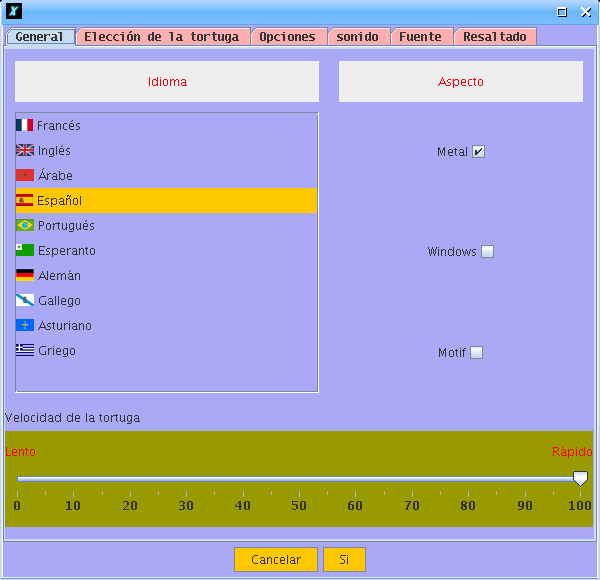
\includegraphics[scale=0.3]{Imagenes/03_Opciones-Menu/Preferencias_01.png}
             \hfill
               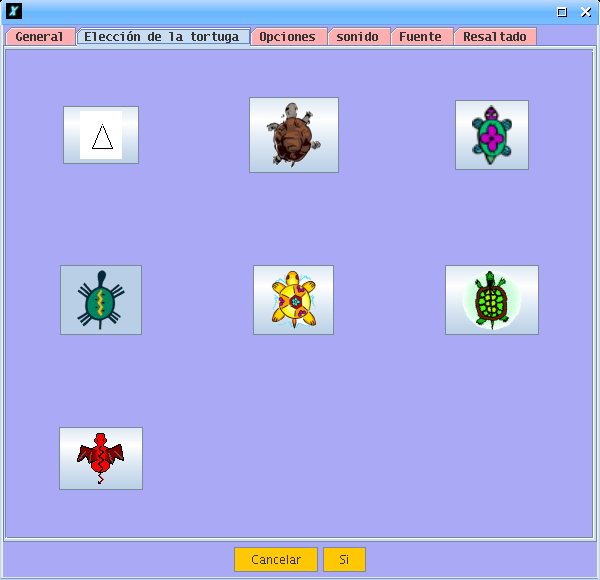
\includegraphics[scale=0.3]{Imagenes/03_Opciones-Menu/Preferencias_02.png}
            \end{center}
         \item \textbf{Elecci\'on de la tortuga}: \index{Figura de la tortuga}
            Elige entre siete tortugas distintas. Tambi\'en accesible con el
            comando \texttt{ponforma} \index{ponforma@\texttt{ponforma}}
            (Secci\'on \ref{Propiedades-Tortuga})
         \item \textbf{Opciones:}
            \begin{center}
               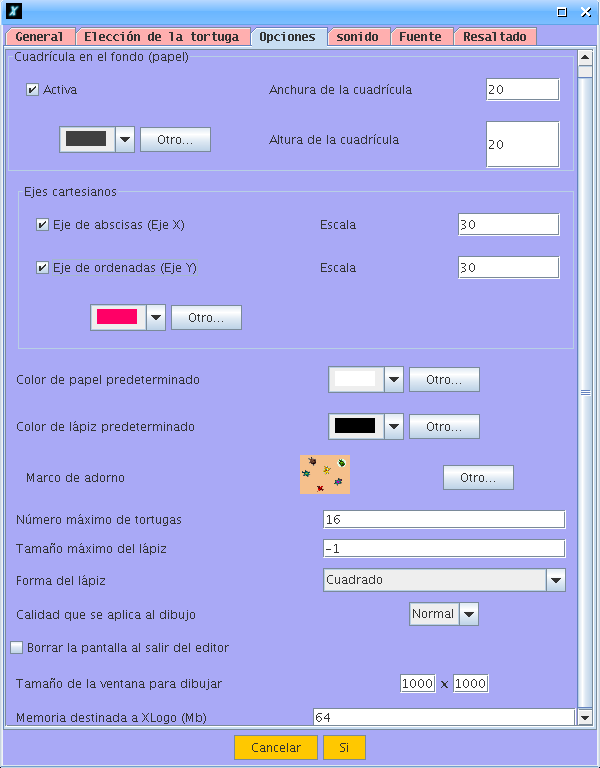
\includegraphics[scale=0.3]{Imagenes/03_Opciones-Menu/Preferencias_03.png}
            \end{center}
            \begin{itemize}
               \item \textbf{Cuadr\'icula en el fondo}:\index{Cuadr\'icula}
                  Establece (o elimina) una cuadr\'icula en el fondo del
                  \'Area de dibujo, as\'i como las medidas y el color de la
                  misma. Tambi\'en accesible con las primitivas 
                  \texttt{cuadricula}\index{cuadricula@\texttt{cuadricula}},
                  \texttt{detienecuadricula} y \texttt{poncolorcuadricula}.
                  \index{detienecuadricula@\texttt{detienecuadricula}}
                  \index{poncolorcuadricula@\texttt{poncolorcuadricula}}
                  (Secci\'on \ref{Propiedades-Tortuga})
               \item \textbf{Ejes cartesianos}:\index{Ejes cartesianos}
                  Muestra (o retira) los ejes cartesianos (X e Y) del \'Area de
                  dibujo, establece su escala (separaci\'on entre marcas) y
                  su color. Tambi\'en accesible con las primitivas
                  \texttt{ejes}\index{ejes@\texttt{ejes}},
                  \texttt{detieneejes}\index{detieneejes@\texttt{detieneejes}},
                  \texttt{ejex}\index{ejex@\texttt{ejex}},
                  \texttt{ejey}\index{ejey@\texttt{ejey}} y
                  \texttt{poncolorejes}\index{poncolorejes@\texttt{poncolorejes}}
                  (Secci\'on \ref{Propiedades-Tortuga}).
               \item \textbf{Color de papel predeterminado}:
                  \index{Color de papel predeterminado} Permite elegir el color
                  por defecto del papel, es decir, el mostrado al iniciar
                  \textsc{XLogo}. 
               \item \textbf{Color de l\'apiz predeterminado}:
                  \index{Color de l\'apiz predeterminado} Permite elegir el color
                  por defecto del l\'apiz, es decir, el utilizado al iniciar
                  \textsc{XLogo}.
               \item \textbf{Marco de adorno}:
                  \index{Marco de adorno} Permite elegir qu\'e marco de adorno
                  se muestra alrededor del \textbf{\'Area de Dibujo}, una
                  imagen o un color s\'olido. Para no superar la memoria
                  asignada, la imagen no puede ocupar m\'as de 100 kb.
                  \begin{center}
                   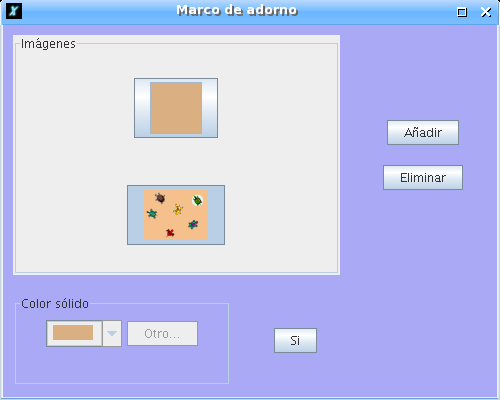
\includegraphics[scale=0.5]{Imagenes/03_Opciones-Menu/Preferencias_Marco.png}
                  \end{center}
               \item \textbf{N\'umero m\'aximo de tortugas}:
                  \index{N\'umero m\'aximo de tortugas} Para el modo
                  multitortuga (secci\'on \ref{Modo-multitortuga}).
                  Por defecto 16.
               \item \textbf{Tama\~no m\'aximo del l\'apiz}:
                  \index{Tama\~no m\'aximo del l\'apiz} Puedes fijar un
                  tama\~no l\'imite para el l\'apiz. Si no se va a utilizar
                  esta limitaci\'on, introduce el n\'umero \texttt{-1} en el
                  recuadro asociado. 
               \item \textbf{Forma del l\'apiz}: \index{Forma del l\'apiz}
                  Cuadrado o Redondo 
               \item \textbf{Tama\~no de la ventana para dibujar}:
                  \index{Tama\~no de la ventana} Puedes establecer un tama\~no
                  personalizado para el \textbf{\'Area de Dibujo}. Por defecto
                  \textsc{XLogo} establece un \'area de 1000 por 1000 pixels.

                  \textbf{Atenci\'on}: seg\'un aumenta el tama\~no de la
                  imagen, puede ser necesario aumentar la memoria destinada
                  a \textsc{XLogo}. Un mensaje de error advertir\'a si ocurre
                  esto.
               \item \textbf{Calidad que se aplica al dibujo}:
                  \index{Calidad del dibujo}Normal, Alto o Bajo. En calidad
                  ``Alta'', no se aprecia ning\'un efecto en
                  particular, pero puede producirse una ralentizaci\'on de la
                  ejecuci\'on.
               \item \textbf{Borrar pantalla al salir del editor}: S\'i o No
               \item \textbf{Tama\~no de la ventana para dibujar}:
                  \index{Tama\~no de la ventana}Determina las dimensiones del
                  \'Area de dibujo.
               \item \textbf{Memoria destinada a \textsc{XLogo}}:
                  \index{Memoria destinada a \textsc{XLogo}} (en Mb) Por
                  defecto, el valor asignado es 64 Mb. Puede ser necesario
                  aumentarlo cuando el tama\~no del \textbf{\'Area de Dibujo}
                  sea demasiado grande. La modificaci\'on de este par\'ametro
                  s\'olo se har\'a efectiva tras cerrar y reiniciar
                  \textsc{XLogo}.

                  \textbf{Atenci\'on}: no aumentar en exceso y/o sin raz\'on
                  este valor, ya que puede ralentizar considerablemente el
                  sistema. Un ejemplo en el que se puede necesitar bastante
                  memoria disponible es al trabajar en el modo 3D com dise\~nos
                  muy complejos.
            \end{itemize}
         \item \textbf{Sonido}: \index{Sonido} La lista de instrumentos que
            puede imitar la tarjeta de sonido a trav\'es de la interfaz
            MIDI. \index{MIDI} Puedes seleccionar un instrumento concreto
            en cualquier momento, mediante la primitiva 
            \texttt{poninstrumento n}.
            \index{poninstrumento@\texttt{poninstrumento}}

            Si usas Windows, esta lista puede estar vac\'ia. Esto se debe
            a que la versi\'on de \textsc{Java} para Windows no incluye los
            \textit{bancos de sonido}, y deben instalarse manualmente. Echa
            un vistazo a la secci\'on \ref{Sonido-Instrumentos-Error}.
            \begin{center}
               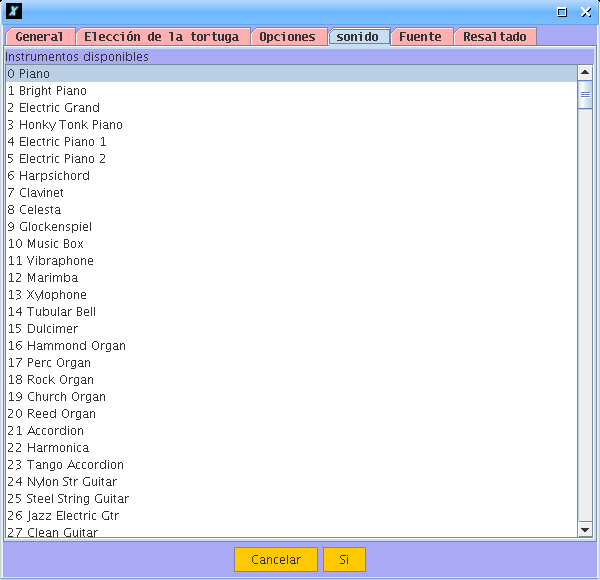
\includegraphics[scale=0.3]{Imagenes/03_Opciones-Menu/Preferencias_04.png}
         \hfill
               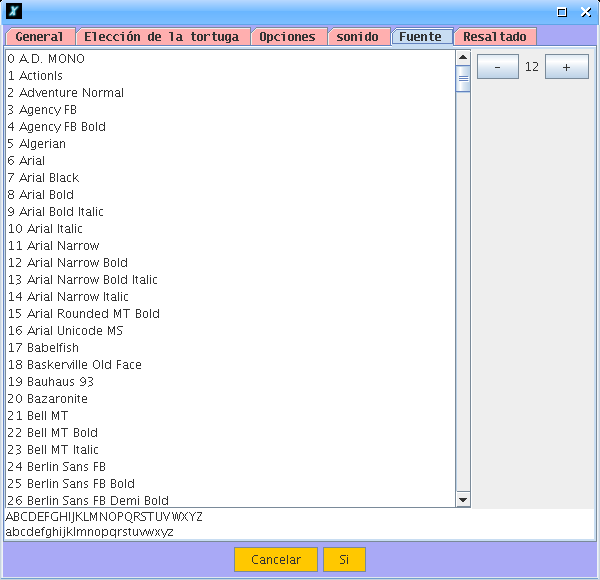
\includegraphics[scale=0.3]{Imagenes/03_Opciones-Menu/Preferencias_05.png}
            \end{center}
         \item \textbf{Fuente}: \index{Fuente} Elige el tipo de letra y su
            tama\~no
            \begin{center}
               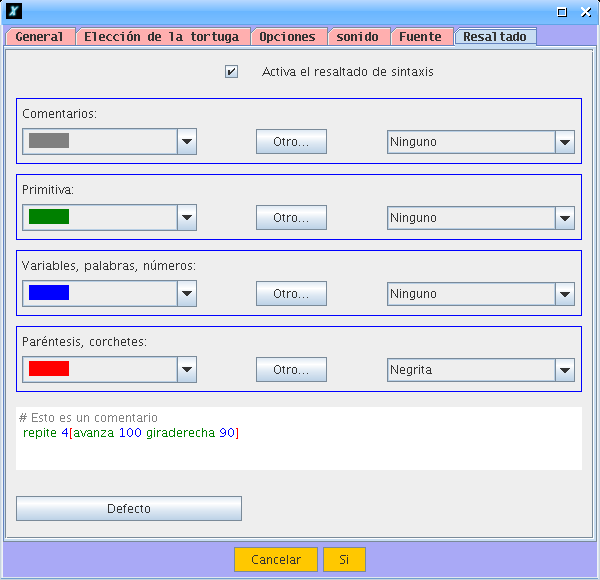
\includegraphics[scale=0.3]{Imagenes/03_Opciones-Menu/Preferencias_06.png}
            \end{center}
         \item \textbf{Resaltado}: \index{Resaltado} Elige los colores que
            se utilizar\'an en el resaltado de primitivas, palabras, variables 
            n\'umeros, par\'entesis y corchetes.
      \end{itemize}
\end{itemize}

\section{Men\'u ``\textit{Ayuda}''}
   \label{Menu-Ayuda}
   \index{Ayuda}

\begin{itemize}
   \item \textbf{Ayuda $\rightarrow$ Licencia}: \index{Licencia GPL}Muestra
      la licencia original GPL (en Ingl\'es) bajo la cual es distribuido este
      programa.
      \begin{center}
         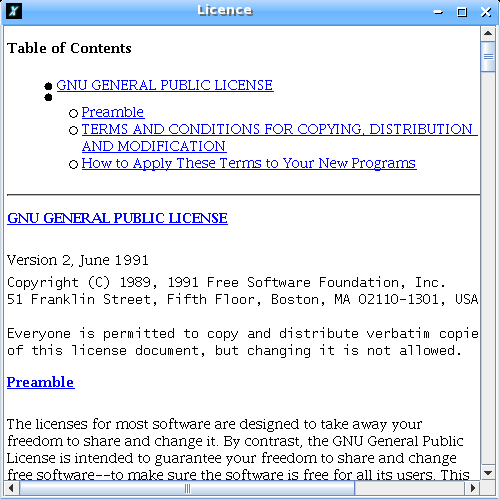
\includegraphics[scale=0.3]{Imagenes/03_Opciones-Menu/Licencia.png}
         \hfill
         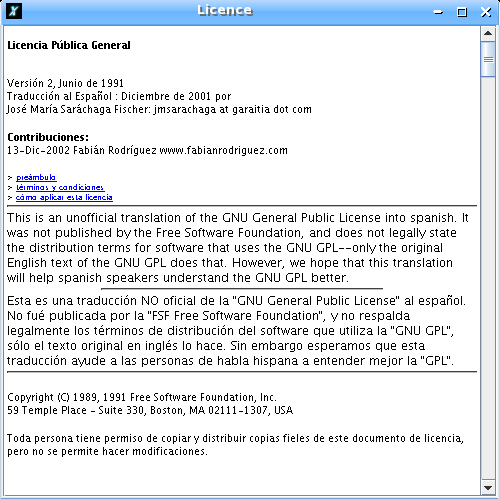
\includegraphics[scale=0.3]{Imagenes/03_Opciones-Menu/Licencia-sp.png}
      \end{center}
   \item \textbf{Ayuda $\rightarrow$ Traducci\'on de la Licencia}:
      \index{Traducci\'on de la Licencia} Refiere a una traducci\'on al
      espa\~nol de la licencia GPL, sin efectos legales, s\'olo como
      referencia para entender la versi\'on en Ingl\'es.
   \item \textbf{Ayuda $\rightarrow$ Traducir XLogo}: \index{Traducir XLogo}
      Abre una ventana para a\~nadir y/o corregir traducciones.
      \begin{center}
         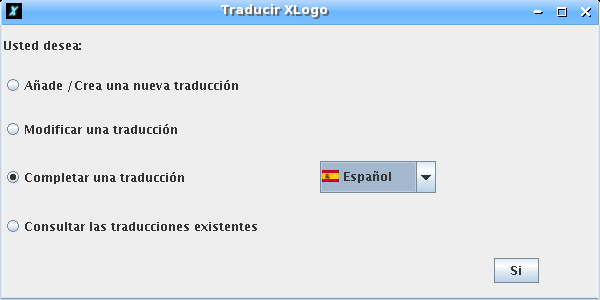
\includegraphics[scale=0.3]{Imagenes/03_Opciones-Menu/Traducir_01.png}
         \hfill
         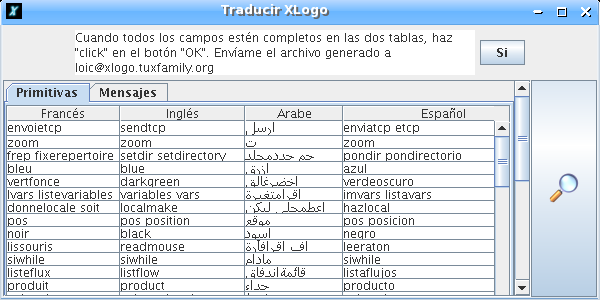
\includegraphics[scale=0.3]{Imagenes/03_Opciones-Menu/Traducir_02.png}
      \end{center}
      Desde ella pueden crearse y/o modificarse tanto las primitivas como
      los mensajes. Una vez creados/modificados, haz \textit{click} 
      \textbf{fuera} de la celda que acabas de escribir y pulsa el bot\'on 
      \texttt{Si}. Se abrir\'a una ventana donde debes elegir el fichero
      de texto donde guardar los cambios y que debes enviar a
      \texttt{loic@xlogo.tuxfamily.org}
      \begin{center}
         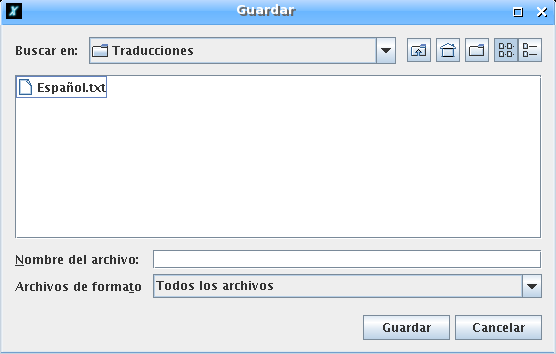
\includegraphics[scale=0.3]{Imagenes/03_Opciones-Menu/Traducir_03.png}
      \end{center}
   \item \textbf{Ayuda $\rightarrow$ Acerca de\ldots{}}: \index{Acerca de ...} Lo de
      siempre \ldots{} y !`!`\texttt{xlogo.tuxfamily.org} para guardar en
      favoritos!! o:)
      \begin{center}
         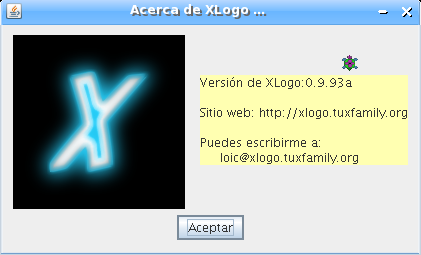
\includegraphics[scale=0.45]{Imagenes/03_Opciones-Menu/Acerca093.png}
      \end{center}
\end{itemize}


\chapter{Convenciones \index{Convenciones} adoptadas para \textsc{XLogo}}
   \label{Convenciones-XLogo}

Esta secci\'on define aspectos claves acerca del lenguaje \textsc{Logo}
en general, y sobre \textsc{XLogo} en particular.

\section{Comandos \index{Comandos} y su interpretaci\'on}
   \label{Comandos}

El lenguaje \textsc{Logo} permite que ciertos eventos sean iniciados
por comandos internos. Estos comandos son llamados
\textit{primitivas}. \index{Primitivas}Cada primitiva puede tener un
cierto n\'umero de par\'ametros que son llamados
\textit{argumentos}. \index{Argumentos}Por ejemplo, la primitiva
\texttt{bp}, que borra la pantalla, no lleva argumentos, mientras
que la primitiva \texttt{suma} tiene dos argumentos.
\begin{quote}
   \texttt{escribe suma 2 3} devuelve \texttt{5}.
\end{quote}
Los argumentos en \textsc{Logo} son de tres tipos:
\begin{itemize}
   \item \textbf{N\'umeros}: \index{N\'umeros} Algunas primitivas esperan
      n\'umeros como su argumento: \texttt{av 100} es un ejemplo.
   \item \textbf{Palabras}: \index{Palabras} Las palabras se escriben
      precedidas por \verb+"+. Un ejemplo de una primitiva que tiene una
      palabra como argumento es \texttt{escribe}. 
      \begin{quote}
         \begin{tabular}{lcccl}
            \verb+escribe "hola+ & & devuelve & & \texttt{hola}
         \end{tabular}
      \end{quote}
      \noindent Nota que si olvidas el \verb+"+, el int\'erprete devuelve
      un mensaje de error. En efecto, \texttt{escribe} esperaba ese argumento,
      pero para el int\'erprete, \texttt{hola} no representa nada, ya que
      no fue definido como n\'umero, ni palabra, ni lista, ni procedimiento. 
   \item \textbf{Listas}: \index{Listas} Se definen encerr\'andolas entre
      corchetes.
\end{itemize}
Los n\'umeros son tratados a veces como un valor (por ej: \texttt{av 100}),
o bien como una palabra (por ejemplo: \texttt{escribe vacio? 12}
devuelve \texttt{falso}). \\

Algunas primitivas tienen una forma general, esto es, pueden ser utilizadas
con n\'umeros o \textit{argumentos opcionales}. \index{Argumentos Opcionales}
Estas primitivas son:
\begin{center} \begin{tabular}{*{4}{c}}
   \texttt{escribe} & \texttt{suma} & \texttt{producto} & \texttt{o} \\
   \texttt{y} & \texttt{lista} & \texttt{frase} & \texttt{palabra} 
\end{tabular} \end{center}
Para que el int\'erprete las considere en su forma general, tenemos que
escribir las \'ordenes entre par\'entesis. Observa los ejemplos:
\begin{verbatim}
   escribe (suma 1 2 3 4 5) \end{verbatim} devuelve:
\begin{verbatim}
   15  \end{verbatim}
Tambi\'en:
\begin{verbatim}
   escribe (lista [a b] 1 [c d]) \end{verbatim} devuelve:
\begin{verbatim}
   [a b] 1 [c d] \end{verbatim}
y
\begin{verbatim}
   si (y 1=1 2=2 8=5+3) [avanza 100 giraderecha 90] \end{verbatim}

\section{Procedimientos}
   \label{Procedimientos}
   \index{Procedimientos}

Adem\'as de las primitivas, puedes definir tus propios comandos. Estos
son llamados \textit{procedimientos}. Los procedimientos son iniciados
por la palabra \texttt{para} \index{para@\texttt{para}} y concluyen
con la palabra \texttt{fin}. \index{fin@\texttt{fin}} Tambi\'en pueden
crearse usando el editor interno de procedimientos \textsc{XLogo}. Veamos
un peque\~no ejemplo:
\begin{verbatim}
   para cuadrado
     repite 4 [
       avanza 100
       giraderecha 90 ]
   fin \end{verbatim}
El proceso para crear el procedimiento es el siguiente:
\begin{enumerate}
   \item Escribir en la \textbf{L\'inea de Comando}: \texttt{para cuadrado}
      y pulsar \texttt{[Enter]}, escribir \texttt{ed} \index{ed@\texttt{ed}}
      y \texttt{[Enter]} o hacer \textit{click} con el rat\'on en el bot\'on 
      \texttt{Editar}
   \item Se mostrar\'a la \textbf{Ventana del Editor},
      \index{Ventana de Editor}donde completamos todo el procedimiento
      \begin{center}
         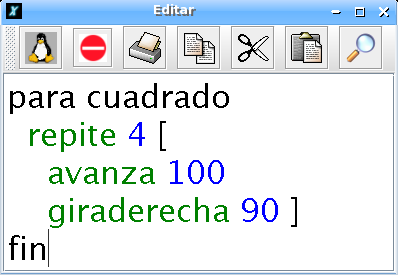
\includegraphics[scale=0.4]{Imagenes/04_Convenciones/EditorProc_01.png}
      \end{center}
   \item Pulsar \includegraphics[scale=0.3]{Imagenes/04_Convenciones/guardar.png} con el
      rat\'on, o hacer \texttt{Alt+Q}
   \item En la ventana del \textbf{Hist\'orico de Comandos},
      \index{Hist\'orico de Comandos} debe aparecer el mensaje:

      \textcolor{blue}{\texttt{Acaba de definir cuadrado}}
      El int\'erprete \textsc{XLogo} no detecta los posibles errores en este
      momento, sino cuando se utilice el procedimiento por primera vez.
   \item Desde ese momento, puede invocarse la orden \texttt{cuadrado} en la
      \textbf{L\'inea de Comandos}
\end{enumerate}
Los procedimientos tambi\'en pueden aprovechar las ventajas de los argumentos.
Para hacer esto, se usan \textit{variables}. \index{Variables} Una
variable es una palabra (un nombre) al que se le puede asignar un valor. 
\begin{quote}
   \noindent \textbf{Ejemplo}:
   \begin{center}
      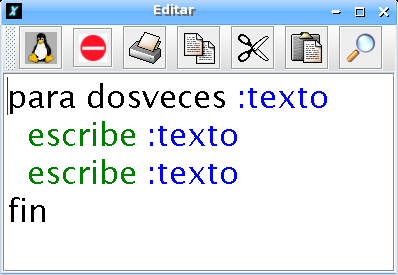
\includegraphics[scale=0.3]{Imagenes/04_Convenciones/EditorProc_02.png}
   \end{center}
   \noindent Probando el ejemplo:
   \begin{verbatim}
  dosveces [1 2 3] \end{verbatim}
   devuelve 
   \begin{verbatim}
  1 2 3
  1 2 3 \end{verbatim}
\end{quote}
Al final del manual se incluyen varios ejemplos de procedimientos.

\section{El caracter especial \textbackslash{}}
   \label{El-caracter-backslash}

El caracter \textbackslash{} (barra invertida o \textit{backslash})
\index{backslash} \index{Barra invertida} permite que las ``palabras''
(secci\'on \ref{Comandos}) contengan espacios \index{Espacios} o
saltos de l\'inea. \index{Saltos de l\'inea}
\begin{itemize}
   \item \verb+\n+ produce un salto de l\'inea
      \index{\textbackslash{}n@\texttt{\textbackslash{}n}}
   \item \verb*+\ + produce un espacio entre palabras
      \index{\verb*+\ +} (\verb*+ + representa un espacio en blanco)
\end{itemize}
\begin{quote}
   \noindent \textbf{Ejemplos}: 

   \begin{tabular}{lcccl}
      \verb+es "xlogo\ xlogo+ & & produce & &
               \texttt{xlogo xlogo} \\
      \verb+es "xlogo\nxlogo+ & & produce & &
         \texttt{xlogo} \\
         & & & & \texttt{xlogo}
   \end{tabular}
\end{quote}
Esto tiene implicaciones a la hora de obtener el caracter \textbackslash{}
en la \textbf{L\'inea de Comandos}: se debe teclear
\verb+\\+.
\index{\textbackslash{}\textbackslash{}@\texttt{\textbackslash{}\textbackslash{}}}
Todo caracter \textbackslash{} es ignorado. Este aviso es importante
en particular para la gesti\'on de archivos 
(secci\'on \ref{Manejo-de-Archivos}). Para establecer como directorio
de trabajo \verb+c:\Mis Documentos+ se debe escribir:
\begin{verbatim}
   pondirectorio "c:\\Mis\ Documentos \end{verbatim}
Nota el uso de \verb*+\ + para indicar el espacio entre
\texttt{Mis} y \texttt{Documentos}. Si se omite el doble
\textit{backslash}, la ruta definida ser\'ia interpretada como:
\begin{verbatim}
   c:Mis Documentos \end{verbatim}
y el int\'erprete mostrar\'a un mensaje de error. 

\section{May\'usculas y min\'usculas}
   \label{Mayusculas-y-minusculas}
   \index{May\'usculas y min\'usculas}

\textsc{XLogo} no distingue entre may\'usculas y min\'usculas en el caso de
nombres de procedimientos y primitivas. As\'i, en el procedimiento
\texttt{cuadrado} como fue definido antes, si escribes \texttt{CUADRADO} o
\texttt{cuAdRAdO}, el int\'erprete de comandos interpretar\'a y ejecutar\'a
correctamente \texttt{cuadrado}. Por otro lado, \textsc{XLogo} s\'i respeta
may\'usculas y min\'usculas en listas y palabras: 
\begin{verbatim}
   escribe "Hola \end{verbatim}
proporciona
\begin{verbatim}
   Hola \end{verbatim}
(la H inicial se mantuvo)

\section{Operadores y sintaxis}
   \label{Operadores-Sintaxis}
   \index{Sintaxis}

Hay dos maneras para escribir ciertos comandos. Por ejemplo, para
sumar 4 y 7, puedes usar la primitiva \texttt{suma} que espera dos
argumentos: 
\begin{verbatim}
   suma 4 7 \end{verbatim}
o puedes usar el operador \texttt{+}: 
\begin{verbatim}
   4 + 7 \end{verbatim}
Ambos tienen el mismo efecto. Esta tabla muestra la relaci\'on entre
operadores y primitivas:

\subsection{Operadores aritm\'eticos}
   \index{Operadores aritm\'eticos}

\begin{center} \begin{tabular}{|*{4}{c|}} \hline 
   \texttt{suma} \index{suma@\texttt{suma}} & 
      \texttt{diferencia} \index{diferencia@\texttt{diferencia}} &
         \texttt{producto} \index{producto@\texttt{producto}} &
            \texttt{divisi\'on} \index{divisi\'on@\texttt{divisi\'on}} \\ \hline
   \texttt{+} & \texttt{--} & * & \texttt{/} \\ \hline
\end{tabular} \end{center}

\subsection{Operadores l\'ogicos}
   \index{Operadores l\'ogicos}

\begin{center} \begin{tabular}{|*{3}{c|}} \hline 
   \texttt{o} \index{o@\texttt{o}} &
      \texttt{y} \index{y@\texttt{y}} &
         \texttt{iguales?} \index{iguales?@\texttt{iguales?}} \\ \hline
   \texttt{|}& \texttt{\&}& \texttt{=} \\ \hline
\end{tabular}\end{center}

\noindent Para comparaciones num\'ericas, disponemos de cuatro operadores sin
primitiva asociada:
\begin{itemize}
   \item El operador ``menor'': \texttt{<}\index{<@\texttt{<}}
   \item El operador ``mayor'': \texttt{>}\index{>@\texttt{>}}
\end{itemize}
Por analog\'ia con otros lenguajes, \textsc{XLogo} incorpora otros dos:
\begin{itemize}
   \item El operador ``menor o igual'': \texttt{<=}\index{<=@\texttt{<=}}
   \item El operador ``mayor o igual'': \texttt{>=}\index{>=@\texttt{>=}}
\end{itemize}
si bien es evidente que no ser\'ian estrictamente necesarios:
\begin{itemize}
   \item \texttt{a <= b} es equivalente a \texttt{no (a > b)} 
   \item \texttt{a >= b} puede sustituirse por \texttt{no (a < b)}
\end{itemize}

\textbf{Nota aclarativa}: Los operadores \texttt{|} y \texttt{\&} son
espec\'ificos de \textsc{XLogo}.\index{\&@\texttt{\&}}\index{=@\texttt{=}}
No se encuentran en otras versiones tradicionales de \textsc{Logo}.
veamos algunos ejemplos de su uso:
\begin{quote} \begin{tabular}{lccccl}
   \texttt{escribe 3+4 = 7-1}      & & devuelve & & \texttt{falso} \\
   \texttt{escribe 3=4 | 7<=49/7}  & & devuelve & & \texttt{cierto} \\
   \texttt{escribe 3=4 \& 7=49/7}  & & devuelve & & \texttt{falso}
\end{tabular} \end{quote}

\section{Las tildes}
\index{Acentuaci\'on y tildes}

Desde la versi\'on 0.9.92 las primitivas en espa\~nol \textsc{XLogo} admiten
tildes. Trat\'andose de un software para uso educativo, es importante que la
ortograf\'ia sea la adecuada.\\

\noindent Para la acentuaci\'on de las primitivas se siguen las normas
ortogr\'aficas habituales, especialmente en aquellas primitivas compuestas
por varias palabras. Por ejemplo:
\begin{itemize}
   \item \texttt{poncolorl\'apiz}. La palabra \texttt{l\'apiz} lleva tilde
      y la mantiene al formar parte de la primitiva, ya que la acentuaci\'on
      de esta recae sobre la ``\texttt{a}'' 
   \item \texttt{leelineaflujo}. Aunque \texttt{l\'inea} lleva tilde al ser
      esdr\'ujula, al pronunciar la primitiva completa, observamos que es
      una palabra llana (el acento se encuentra en la ``\texttt{u}'' de
      \texttt{flujo}), as\'i que no se le asigna tilde.

      S\'i que lleva tilde en \texttt{definel\'inea} y \texttt{finl\'inea},
      por el mismo motivo explicado antes para \texttt{l\'apiz}
   \item Se procede del mismo modo en las formas cortas de las primitivas.
      Las formas cortas de \texttt{definepol\'igono} y \texttt{finpol\'igono}
      son, respectivamente, \texttt{defpoli} y \texttt{finpoli}.
      Escuchando a los alumnos pronunciarlas, se opt\'o por considerarlas
      llanas y sin tilde.
\end{itemize}

Dicho lo anterior, debemos tener una idea sobre la distinta codificaci\'on
de caracteres que usan los Sistemas Operativos. \\

La codificaci\'on de caracteres es el m\'etodo que convierte un car\'acter de
un lenguaje natural en un c\'odigo num\'erico. Es muy habitual (m\'as de lo
que ser\'ia deseable) que los sistemas operativos (Windows, Linux, MacOS,
Solaris, \ldots) usen distintos sistemas de codificaci\'on. Existen varias
normas: ASCII, Unicode, UTF, ISO, \ldots, y eso afecta negativamente a los
caracteres especiales del espa\~nol:
\begin{itemize}
   \item Vocales acentuadas: \'a, \'e, \'i, \'o, \'u
   \item Letras e\~ne y ``cedilla'': \~n y \c{c}
   \item Apertura de exclamaci\'on, interrogaci\'on, \ldots: ?`, !` , \ldots.
\end{itemize}

Si tienes intenci\'on de compartir tus programas por Internet, intenta evitar
estos caracteres y utiliza primitivas sin tilde. Si est\'as en una aula,
recomendamos el uso acentuado de las mismas.

\chapter{Listado de primitivas}
   \label{Listado-Primitivas}
   \index{Listado de primitivas}

Como dec\'iamos, la tortuga se controla por medio de comandos internos
llamados \textit{primitivas}. Las siguientes secciones definen estas
primitivas:

\section{Movimientos de la tortuga; poner l\'apiz y colores}
   \label{Movimientos-Colores}

\subsection{Movimientos}
   \label{Movimientos}

Esta primera tabla define las primitivas que gobiernan el movimiento
de la tortuga, y s\'olo necesitan un argumento:
\begin{center}
 \begin{longtable}{*{2}{|m{3cm}}|m{9cm}|} \hline
   \multicolumn{1}{|c|}{\textbf{Primitivas}} & 
      \multicolumn{1}{c|}{\textbf{Argumentos}} &
         \multicolumn{1}{c|}{\textbf{Uso}} \\ \endhead \hline 
   \texttt{avanza}, \index{avanza@\texttt{avanza}}
     \texttt{av} \index{av@\texttt{av}} & \texttt{n: n\'umero de pasos} &
          Mueve la tortuga hacia adelante \texttt{n} pasos en la
          direcci\'on que actualmente est\'a mirando. \\ \hline 
   \texttt{retrocede}, \index{retrocede@\texttt{retrocede}}
     \texttt{re} \index{re@\texttt{re}} & \texttt{n: n\'umero de pasos} &
          Mueve la tortuga hacia atr\'as \texttt{n} pasos en la direcci\'on
          que actualmente est\'a mirando. \\ \hline 
   \texttt{giraderecha}, \index{giraderecha@\texttt{giraderecha}}
     \texttt{gd} \index{gd@\texttt{gd}} & \texttt{n: \'angulo} &
          Gira la tortuga \texttt{n} grados hacia la derecha de la direcci\'on
          que actualmente est\'a mirando. \\ \hline 
   \texttt{giraizquierda}, \index{giraizquierda@\texttt{giraizquierda}}
     \texttt{gi} \index{gi@\texttt{gi}} & \texttt{n: \'angulo} &
          Gira la tortuga \texttt{n} grados hacia la izquierda de la
          direcci\'on que actualmente est\'a mirando. \\ \hline 
\end{longtable} \end{center}

En esta segunda tabla el movimiento se controla mediante \textbf{coordenadas} en
la pantalla. Para ver mejor dichas coordenadas, se dispone de las primitivas
\texttt{cuadr\'icula}, que muestra una cuadr\'icula en pantalla de las dimensiones
deseadas, y \texttt{ejes}, que muestra los ejes cartesianos con las correspondientes 
etiquetas: 
\begin{center}
 \begin{longtable}{|m{3.5cm}|m{3cm}|m{8.5cm}|} \hline
   \multicolumn{1}{|c|}{\textbf{Primitivas}} & 
      \multicolumn{1}{c|}{\textbf{Argumentos}} &
         \multicolumn{1}{c|}{\textbf{Uso}} \\ \endhead \hline
   \texttt{cuadr\'icula} \index{cuadr\'icula@\texttt{cuadr\'icula}} &
      \texttt{a b: n\'umeros} &
        Dibuja una cuadr\'icula en el \textbf{\'Area de dibujo} de dimensiones 
         \texttt{a} x \texttt{b} y borra la pantalla\\ \hline
   \texttt{borracuadr\'icula}\index{borracuadr\'icula@\texttt{borracuadr\'icula}}
%   \texttt{detienecuadr\'icula}\index{detienecuadr\'icula@\texttt{detienecuadr\'icula}}
      & \texttt{no} &
        Quita la cuadr\'icula del \textbf{\'Area de dibujo} y borra la pantalla
          \\ \hline
 \texttt{poncolorcuadr\'icula}\index{poncolorcuadr\'icula@\texttt{poncolorcuadr\'icula}}
      \texttt{pcc}\index{pcc@\texttt{pcc}} &
      \texttt{primitiva}, \texttt{lista} o \texttt{numero} &
        Establece el color de la cuadr\'icula del \textbf{\'Area de dibujo}
          \\ \hline
   \texttt{colorcuadr\'icula}\index{colorcuadr\'icula@\texttt{colorcuadr\'icula}} & 
      \texttt{no} &
        Devuelve el color actual de la cuadr\'icula. \\ \hline
   \texttt{ejes}\index{ejes@\texttt{ejes}}&
      \texttt{a: n\'umero}  &
        Dibuja los ejes cartesianos (X e Y) de escala (separaci\'on entre marcas)
        \texttt{a}, con las etiquetas correspondientes.
          \\ \hline
   \texttt{ejex}\index{ejex@\texttt{ejex}}&
      \texttt{a: n\'umero}  &
        Dibuja el eje de abscisas (eje X) de escala (separaci\'on entre marcas)
        \texttt{a}, con las etiquetas correspondientes.
          \\ \hline
   \texttt{ejey}\index{ejey@\texttt{ejey}}&
      \texttt{a: n\'umero}  &
        Dibuja el eje de ordenadas (eje Y) de escala (separaci\'on entre marcas)
        \texttt{a}, con las etiquetas correspondientes.
          \\ \hline
   \texttt{borraejes}\index{borraejes@\texttt{borraejes}}
%   \texttt{detieneejes}\index{detieneejes@\texttt{detieneejes}}
      & \texttt{no}  &
        Quita los ejes del \textbf{\'Area de dibujo} y borra la pantalla
            \\ \hline
   \texttt{poncolorejes}\index{poncolorejes@\texttt{poncolorejes}}
      \texttt{pce}\index{pce@\texttt{pce}} &
      \texttt{primitiva}, \texttt{lista} o \texttt{numero} &
        Establece el color de los ejes en el \textbf{\'Area de dibujo}
            \\ \hline
   \texttt{colorejes}\index{colorejes@\texttt{colorejes}} &
      \texttt{no} &
        Devuelve el color actual de los ejes. \\ \hline \hline
   \texttt{centro} \index{centro@\texttt{centro}} & \texttt{no} &
          Lleva la tortuga a la posici\'on original, es decir coordenadas
          \texttt{[0 0]} con rumbo \texttt{0}. \\ \hline 
   \texttt{posici\'on}, \index{posici\'on@\texttt{posici\'on}} 
      \texttt{pos} \index{pos@\texttt{pos}} & \texttt{no} &
        Devuelve las coordenadas X e Y de la posici\'on actual
        de la tortuga.\\ \hline 
   \texttt{ponposici\'on}, \index{ponposici\'on@\texttt{ponposici\'on}}
     \texttt{ponpos} \index{ponpos@\texttt{ponpos}} &
        \texttt{[x y]: lista de dos n\'umeros}&
          Mueve la tortuga a las coordenadas especificadas por los dos
          n\'umeros en la lista (\texttt{x} es la abscisa, \texttt{y} la
          ordenada). \\ \hline 
   \texttt{ponx} \index{ponx@\texttt{ponx}} & \texttt{x: eje x} &
          Mueve la tortuga horizontalmente hasta el punto de abscisa \texttt{x}
                 \\ \hline 
   \texttt{pony} \index{pony@\texttt{pony}} & \texttt{y: eje y} &
          Mueve la tortuga verticalmente hasta el punto de ordenada \texttt{y}
                  \\ \hline 
   \texttt{ponxy} \index{ponxy@\texttt{ponxy}} & 
       \texttt{x y}: coordenadas \texttt{x} e \texttt{y} &
          Id\'entico a \texttt{ponpos [x y]} \texttt{x} e \texttt{y} son
          n\'umeros, no una lista. \\ \hline 
   \texttt{punto} \index{punto@\texttt{punto}} & \texttt{a: lista} &
          El punto definido por las coordenadas de la lista se resaltar\'a
          con el color del l\'apiz. \\ \hline
\end{longtable} \end{center}

Esta tercera tabla muestra las primitivas que controlan el rumbo, direcci\'on
en grados respecto de la vertical y mirando hacia arriba:
\begin{center}
 \begin{longtable}{*{2}{|m{3cm}}|m{9cm}|} \hline
   \multicolumn{1}{|c|}{\textbf{Primitivas}} & 
      \multicolumn{1}{c|}{\textbf{Argumentos}} &
         \multicolumn{1}{c|}{\textbf{Uso}} \\ \endhead \hline
   \texttt{rumbo} \index{rumbo@\texttt{rumbo}} & \texttt{no} &
        Devuelve el rumbo o el \'angulo de la tortuga.\\ \hline 
   \texttt{ponrumbo}, \index{ponrumbo@\texttt{ponrumbo}} 
     \texttt{ponr} \index{ponr@\texttt{ponr}} & \texttt{n: rumbo} &
          Orienta la tortuga en la direcci\'on especificada. \texttt{0}
          corresponde a mirar hacia arriba verticalmente. \\ \hline 
   \texttt{hacia} \index{hacia@\texttt{hacia}} & \texttt{a: lista} &
        La lista debe contener dos n\'umeros que representen coordenadas.
        Devuelve el rumbo que la tortuga deber\'a seguir hacia el punto
        definido por las coordenadas.\\ \hline 
   \texttt{distancia} \index{distancia@\texttt{distancia}} & 
      \texttt{a: lista} &
        La lista debe contener dos n\'umeros que representen coordenadas.
        Devuelve el n\'umero de pasos desde la actual posici\'on y el punto
        definido por las coordenadas.\\ \hline 
\end{longtable} \end{center}

\subsection{Propiedades}
   \label{Propiedades-Tortuga}
   \index{Propiedades}

Esta tabla descrine las primitivas que permiten ajustar las propiedades de la
tortuga. Por ejemplo, ?`estar\'a visible en la pantalla? ?`Con qu\'e color
dibujar\'a cuando se mueva?

\begin{center} \begin{longtable}{*{2}{|m{3cm}}|m{9cm}|} \hline  
    \multicolumn{1}{|c|}{\textbf{Primitivas}} &
       \multicolumn{1}{c|}{\textbf{Argumentos}} &
          \multicolumn{1}{c|}{\textbf{Uso}} \\ \endhead \hline 
   \texttt{muestratortuga}, \index{muestratortuga@\texttt{muestratortuga}}
     \texttt{mt} \index{mt@\texttt{mt}} & \texttt{no} &
        Hace que la tortuga se vea en pantalla. \\ \hline 
   \texttt{ocultatortuga}, \index{ocultatortuga@\texttt{ocultatortuga}}
     \texttt{ot} \index{ot@\texttt{ot}} & \texttt{no} &
        Hace invisible a la tortuga. \\ \hline 
   \texttt{bajal\'apiz}, \index{bajal\'apiz@\texttt{bajal\'apiz}}
     \texttt{bl} \index{bl@\texttt{bl}} & \texttt{no} &
        La tortuga dibujar\'a una l\'inea cuando se mueva. \\ \hline 
   \texttt{subel\'apiz}, \index{subel\'apiz@\texttt{subel\'apiz}}
     \texttt{sl} \index{sl@\texttt{sl}} & \texttt{no} &
        La tortuga no dibujar\'a cuando se mueva. \\ \hline 
   \texttt{goma}, \index{goma@\texttt{goma}}
     \texttt{go} \index{go@\texttt{go}} & \texttt{no} &
        La tortuga borrar\'a toda traza que encuentre.\\ \hline 
   \texttt{inviertel\'apiz}, \index{inviertel\'apiz@\texttt{inviertel\'apiz}}
     \texttt{ila} \index{ila@\texttt{ila}} & \texttt{no} &
        Pone la tortuga en ``modo inverso'', y l\'apiz abajo.
              \\ \hline 
   \texttt{ponl\'apiz}, \index{ponl\'apiz@\texttt{ponl\'apiz}}
     \texttt{pla} \index{pla@\texttt{pla}} & \texttt{no} &
        Pone la tortuga en el modo normal de dibujo y l\'apiz abajo. \\ \hline 
   \texttt{poncolorl\'apiz}, \index{poncolorl\'apiz@\texttt{poncolorl\'apiz}}
     \texttt{poncl} \index{poncl@\texttt{poncl}} & 
        \texttt{a: n\'umero, primitiva o lista [r v a]} &
           Cambia el color del l\'apiz.
           La especificaci\'on del color se detalla en la secci\'on
            \ref{AcercaColores} \\ \hline 
   \texttt{pongrosor} \index{pongrosor@\texttt{pongrosor}} & 
      \texttt{n: n\'umero} &
        Define el grosor del trazo del l\'apiz (en pixels). Por defecto es 1.
        La forma es cuadrada.\\ \hline 
   \texttt{colorl\'apiz}, \index{colorl\'apiz@\texttt{colorl\'apiz}}
     \texttt{cl} \index{cl@\texttt{cl}} & \texttt{a: lista} &
        Devuelve el color actual del l\'apiz. \\ \hline 
   \texttt{encuentracolor}, \index{encuentracolor@\texttt{encuentracolor}}
     \texttt{ec} \index{ec@\texttt{ec}} & \texttt{a: lista} &
        Devuelve el color del punto definido por las coordenadas. \\ \hline
   \texttt{grosorl\'apiz}, \index{grosorl\'apiz@\texttt{grosorl\'apiz}}
   \texttt{gl} \index{gl@\texttt{gl}} & \texttt{no} &
        Devuelve el grosor del l\'apiz. \\ \hline 
   \texttt{ponformal\'apiz}, \index{ponformal\'apiz@\texttt{ponformal\'apiz}}
   \texttt{pfl} \index{pfl@\texttt{pfl}} & \texttt{n: 0 \'o 1} &
        Fija la forma del l\'apiz: \texttt{pfl 0}: cuadrada; 
        \texttt{pfl 1}: ovalada. \\ \hline 
   \texttt{formal\'apiz}, \index{formal\'apiz@\texttt{formal\'apiz}}
   \texttt{fl} \index{fl@\texttt{fl}} & \texttt{no} &
        Devuelve la forma del l\'apiz. \\ \hline 
   \texttt{ponforma}, \index{ponforma@\texttt{ponforma}} 
      \texttt{pforma} \index{pforma@\texttt{pforma}} & \texttt{n: n\'umero} &
        Puedes elegir tu tortuga preferida en la segunda etiqueta del men\'u
        \textbf{Herramientas $\rightarrow$ Preferencias}, pero tambi\'en es posible
        con \texttt{ponforma}. El n\'umero \texttt{n} puede ir de 0 a 6. (0 es 
        la forma triangular del \textsc{Logo} tradicional). \\ \hline 
   \texttt{forma} \index{forma@\texttt{forma}} & \texttt{no} &
        Devuelve un n\'umero que representa la forma actual de la tortuga.
           \\ \hline 
\end{longtable} \end{center}

El control del \'Area de dibujo se realiza con las primitivas siguientes:
\begin{center} \begin{longtable}{|m{3.5cm}|m{3cm}|m{8.5cm}|} \hline  
    \multicolumn{1}{|c|}{\textbf{Primitivas}} &
       \multicolumn{1}{c|}{\textbf{Argumentos}} &
          \multicolumn{1}{c|}{\textbf{Uso}} \\ \endhead \hline 
   \texttt{poncolorpapel}, \index{poncolorpapel@\texttt{poncolorpapel}}
     \texttt{poncp} \index{poncp@\texttt{poncp}} & 
        \texttt{a: n\'umero, primitiva o lista [r v a]} &
           Cambia el color del papel (fondo).
           La especificaci\'on del color se detalla en la secci\'on
            \ref{AcercaColores} \\ \hline 
   \texttt{colorpapel} \index{colorpapel@\texttt{colorpapel}} &
     \texttt{a: lista} &
        Devuelve el color actual del ``papel'' (fondo, \'area
        de dibujo). \\ \hline 
   \texttt{poncalidaddibujo}, \index{poncalidaddibujo@\texttt{poncalidaddibujo}} 
   \texttt{pcd} \index{pcd@\texttt{pcd}}  & \texttt{n: 0, 1 \'o 2} &
        Fija la calidad del dibujo: \texttt{pcd 0}: normal;
         \texttt{pcd 1}: alta; \texttt{pcd 2}: baja; \\ \hline  
   \texttt{calidaddibujo}, \index{calidaddibujo@\texttt{calidaddibujo}}
   \texttt{cdib} \index{cdib@\texttt{cdib}} & \texttt{no} &
        Devuelve la calidad del dibujo \\ \hline 
   \texttt{tama\~nopantalla}, \index{tama\~nopantalla@\texttt{tama\~nopantalla}}
   \texttt{tpant} \index{tpant@\texttt{tpant}} & \texttt{no} &
        Devuelve una lista que contiene el tama\~no de la pantalla \\ \hline 
   \texttt{pontama\~nopantalla}
       \index{pontama\~nopantalla@\texttt{pontama\~nopantalla}}
   \texttt{ptp} \index{@ptp\texttt{ptp}} & \texttt{a: lista} &
        Fija el tama\~no de la pantalla. Ejemplo: \texttt{ptp [1000 1000]} \\ \hline
   \texttt{modoventana} \index{modoventana@\texttt{modoventana}} &
      \texttt{no} &
        La tortuga puede salir del \'area de dibujo (pero no dibujar\'a nada).
           \\ \hline 
   \texttt{modovuelta} \index{modovuelta@\texttt{modovuelta}} & \texttt{no} &
        Si la tortuga sale del \'area de dibujo, vuelve a aparecer en el lado
        opuesto \\ \hline 
   \texttt{modojaula} \index{modojaula@\texttt{modojaula}} & \texttt{no} &
        La tortuga queda confinada al \'area de dibujo. Si intenta salir,
        aparecer\'a un mensaje de error avisando cu\'antos pasos faltan
        para el punto de salida. \\ \hline 
   \texttt{tama\~noventana}, \index{tama\~noventana@\texttt{tama\~noventana}} 
     \texttt{tv}, \index{tv@\texttt{tv}}
   \texttt{esquinasventana} \index{esquinasventana@\texttt{esquinasventana}} &
      \texttt{no} &
        Devuelve una lista con cuatro elementos, las coordenadas de la esquina
        superior izquierda y de la esquina inferior derecha.

        Por ejemplo, si devuelve \texttt{[-200 200 400 -300]}, significa que
        las coordenadas de la esquina superior izquierda son \texttt{(-200,200)}
        y las de la esquina inferior derecha \texttt{(400,-300)}\\ \hline 
   \texttt{zoom} \index{zoom@\texttt{zoom}} &
      \texttt{a: n\'umero} &
        Acerca o aleja el \'Area de dibujo. En concreto, el valor de \texttt{a}
        es el factor de escala respecto a la imagen original:
        \texttt{(a>1)} acerca el \'Area de dibujo;  
        \texttt{(0<a<1)} aleja el \'Area de dibujo. \\ \hline
   \texttt{borrapantalla}, \index{borrapantalla@\texttt{borrapantalla}}
     \texttt{bp} \index{bp@\texttt{bp}} & \texttt{no} &
        Vac\'ia el \'area de dibujo, situando a la tortuga en el centro de
        la pantalla. \\ \hline 
   \texttt{limpia} \index{limpia@\texttt{limpia}} & \texttt{no} &
        Vac\'ia el \'area de dibujo, dejando a la tortuga en el lugar donde
        estaba tras la ejecuci\'on anterior.\\ \hline 
\end{longtable} \end{center}

Finalmente, las primitivas que controlan la escritura en pantalla, los mensajes
al usuario y simplifican determinados dibujos:
\begin{center} \begin{longtable}{*{2}{|m{3cm}}|m{9cm}|} \hline  
    \multicolumn{1}{|c|}{\textbf{Primitivas}} &
       \multicolumn{1}{c|}{\textbf{Argumentos}} &
          \multicolumn{1}{c|}{\textbf{Uso}} \\ \endhead \hline 
   \texttt{rotula} \index{rotula@\texttt{rotula}} & 
       \texttt{a: palabra o lista} & 
          Dibuja la palabra o lista especificada, en la posici\'on actual,
          y en la direcci\'on que est\'a mirando. \\ \hline 
   \texttt{largoetiqueta}
       \index{largoetiqueta@\texttt{largoetiqueta}} & \texttt{a: lista} &
          Devuelve, en p\'ixels, la longitud que tendr\'a en pantalla la
          lista. \\ \hline
   \texttt{ponfuente}, \index{ponfuente@\texttt{ponfuente}}
     \texttt{pf} \index{pf@\texttt{pf}} & \texttt{n: n\'umero} &
        Cuando se escribe con la primitiva \texttt{rotula}, modifica el tama\~no
        de la tipograf\'ia. Por defecto, el tama\~no es 12. \\ \hline 
   \texttt{fuente} \index{fuente@\texttt{fuente}} & \texttt{no} &
        Devuelve el tama\~no de la tipograf\'ia cuando se escribe en pantalla
        con la primitiva rotula. \\ \hline 
   \texttt{mensaje}, \index{mensaje@\texttt{mensaje}}
     \texttt{msj}\index{msj@\texttt{msj}} & \texttt{a: lista} &
        Muestra una caja de di\'alogo con el mensaje que est\'a en la lista.
        El programa se detiene hasta que el usuario hace un \textit{click} en
        el bot\'on ``Aceptar'' \\ \hline
   \texttt{c\'irculo} \index{c\'irculo@\texttt{c\'irculo}} & \texttt{n: radio} &
          Dibuja una circunferencia de radio \texttt{n} alrededor de la
          tortuga \\ \hline 
   \texttt{arco} \index{arco@\texttt{arco}} & \texttt{n: radio}
                                                \texttt{a~b:~\'angulos} &
          Dibuja un arco de circunferencia de radio \texttt{n} alrededor
          de la tortuga, comprendido entre los \'angulos \texttt{a} y
          \texttt{b}, midiendo desde el rumbo de la tortuga. \\ \hline 
\end{longtable}\end{center}

La primitiva \texttt{largoetiqueta} permite saber si al escribir en
pantalla con \texttt{rotula} tienes suficiente espacio.
\begin{quote}
   \noindent \textbf{Ejemplo}:

   \texttt{largoetiqueta [Hola, ?`c\'omo est\'as?]} devuelve, en p\'ixels
   la longitud en pantalla de la frase \textit{Hola, ?`c\'omo est\'as?} 
\end{quote}

\subsection{La tortuga en Tres Dimensiones}
   \label{3-Dimensiones}
   \index{3d} \index{Tres Dimensiones}

Desde la versi\'on 0.9.92, nuestra tortuga puede dejar el plano para trasladarse
a un espacio en tres dimensiones (3D). Para cambiar a esta modalidad,
Usaremos la primitiva \texttt{perspectiva}. !`Bienvenido a un mundo en 3D!
\index{perspectiva@\texttt{perspectiva}}

Para recuperar el modo bidimensional (2D), debemos indicarle que vuelva a uno
de los modos ``planos'': \texttt{modojaula}, \texttt{modoventana} o 
\texttt{modovuelta}. \index{modojaula@\texttt{modojaula}}
\index{modovuelta@\texttt{modovuelta}}\index{modoventana@\texttt{modoventana}}

\subsubsection{La proyecci\'on en perspectiva}

Para representar un espacio 3D en un plano 2D, \textsc{Xlogo} utiliza una
proyecci\'on en perspectiva. Es equivalente a tener una c\'amara grabando
la escena en 3D, y mostrando en la pantalla la imagen de la proyecci\'on.
Veamos un esquema gr\'afico para explicarlo mejor:
\begin{center}
   \includegraphics[scale=0.5]{Imagenes/05_Primitivas/Perspectiva01.png}
\end{center}

Disponemos de primitivas para fijar la posici\'on de la c\'amara, mientras
que la pantalla de proyecci\'on se encuentra en el punto medio entre la c\'amara
y el objeto.

\subsubsection{Entender la orientaci\'on en el mundo tridimensional}

En el plano, la tortuga la orientaci\'on se define \'unicamente por su rumbo.
Sin embargo, en el mundo tridimensional la orientaci\'on de la tortuga necesita
de tres \'angulos. Si usamos la orientaci\'on por defecto de la tortuga en 3D
(en el plano \texttt{XY} mirando hacia el semieje \texttt{Y} positivo):
\begin{description}
   \item[Balanceo:] la rotaci\'on en torno al eje \texttt{OY}
   \item[Cabeceo:] la rotaci\'on seg\'un el eje \texttt{OX}
   \item[Rumbo:] la rotaci\'on seg\'un el eje \texttt{OZ}
\end{description}
De hecho, para moverse en el mundo tridimiensional, la tortuga se comportar\'a 
de modo muy similar a un avi\'on. De nuevo, ilustremos con una imagen los 3
\'angulos:
\begin{center} \begin{tabular}{ccccc}
   \includegraphics[scale=0.25]{Imagenes/05_Primitivas/plane-balanceo.png} & &
     \includegraphics[scale=0.3]{Imagenes/05_Primitivas/plane-cabeceo.png} & &
       \includegraphics[scale=0.25]{Imagenes/05_Primitivas/plane-rumbo.png} \\*[0.3cm]
   \textbf{Balanceo} & & \textbf{Cabeceo} & & \textbf{Rumbo} 
\end{tabular} \end{center}

Parece bastante complicado la primera vez que se estudia, pero veremos que
muchas cosas son similares a los movimientos en el plano bidimensional. Estas
son las primitivas b\'asicas para moverse en el mundo 3D:
\begin{itemize}
   \item \texttt{avanza}, \texttt{retrocede}, \texttt{av}, \texttt{re}:
      \index{avanza@\texttt{avanza}}\index{retrocede@\texttt{retrocede}}%
      \index{av@\texttt{av}}\index{re@\texttt{re}}Id\'enticas al mundo 2D
   \item \texttt{giraderecha}, \texttt{giraizquierda}, \texttt{gd}, \texttt{gi}:
      \index{giraderecha@\texttt{giraderecha}}\index{gd@\texttt{gd}}%
      \index{giraizquierda@\texttt{giraizquierda}}\index{gi@\texttt{gi}}%
      Id\'enticas al mundo 2D, producen una rotaci\'on alrededor del eje
      transversal y vertical de la tortuga
   \item \texttt{balanceaderecha}, \texttt{bd}:
      \index{balanceaderecha@\texttt{balanceaderecha}}\index{bd@\texttt{bd}}%
      la tortuga gira \texttt{n} grados a la derecha respecto a su eje
      longitudinal 
   \item \texttt{balanceaizquierda}, \texttt{bi}:%
      \index{balanceizquierda@\texttt{balanceaizquierda}}\index{bi@\texttt{bi}}
      la tortuga gira \texttt{n} grados a la izquierda respecto a su eje
      longitudinal 
   \item \texttt{cabeceaarriba}, \texttt{subenariz}, \texttt{sn}:%
      \index{cabeceaarriba@\texttt{cabecearriba}}\index{sn@\texttt{sn}}%
      \index{subenariz@\texttt{subenariz}} La tortuga ``sube el morro''
      \texttt{n} grados respecto a su eje transversal y horizontal
   \item \texttt{cabeceaabajo}, \texttt{bajanariz}, \texttt{bn}:%
      \index{cabeceaabajo@\texttt{cabeceabajo}}\index{bn@\texttt{bn}}%
      \index{bajanariz@\texttt{bajanariz}} La tortuga ``baja el morro''
      \texttt{n} grados respecto a su eje transversal y horizontal
\end{itemize}

En el plano bidimensional, para dibujar un cuadrado de \texttt{200} pasos
de tortuga, escribimos:
\begin{verbatim}
 repite 4 [ avanza 200 giraderecha 90 ]\end{verbatim}
Estas \'ordenes siguen existiendo el mundo 3D, y el cuadrado puede
dibujarse perfectamente en modo \texttt{perspectiva}. 

\parbox{9cm}{
Si la tortuga baja ``el morro'' 90 grados, podemos dibujar otro
cuadrado, y obtenemos:\\*[0.3cm]
\texttt{borrapantalla}\\
\texttt{repite 4 [ avanza 200 giraderecha 90 ]}\\
\texttt{bajanariz 90}\\
\texttt{repite 4 [ avanza 200 giraderecha 90 ]}} \hfill 
\parbox{7cm}{\begin{center}
   \includegraphics[scale=0.5]{Imagenes/05_Primitivas/Perspectiva02.png}
\end{center} }

Puedes (debes) probar otros ejemplos para entender perfectamente la
orientaci\'on de la tortuga y el uso de los \'angulos y !`convertirte en
un experto! \\

\noindent Tambi\'en debes entender que las tres primitivas que controlan la
rotaci\'on en 3D est\'an relacionadas entre s\'i; por ejemplo, al ejecutar:
\begin{verbatim}
 borrapantalla
 balanceaizquierda 90 subenariz 90 balanceaderecha 90\end{verbatim}
El movimiento de la tortuga es equivalente a:
\begin{verbatim}
 giraizquierda 90\end{verbatim}
(Puedes probar con tu mano si no lo entiendes bien)

\subsubsection{Primitivas disponibles tanto en 2D como 3D}

Las siguientes primitivas est\'an disponibles tanto en el plano como en
el mundo 3D. La \'unica diferencia son los argumentos admitidos por las
primitivas. \\

\noindent Estas precisan de los mismos argumentos que en el plano:
\begin{center}\begin{tabular}{ccccc}
   \texttt{c\'irculo}\index{c\'irculo@\texttt{c\'irculo}}    & &
   \texttt{arco}\index{arco@\texttt{arco}}             & &
   \texttt{centro}\index{centro@\texttt{centro}}       \\
   \texttt{ponx}\index{ponx@\texttt{ponx}}             & &
   \texttt{pony}\index{pony@\texttt{pony}}             & &
   \texttt{rumbo}\index{rumbo@\texttt{rumbo}}          \\
   \texttt{ponrumbo}\index{ponrumbo@\texttt{ponrumbo}} & &
   \texttt{rotula}\index{rotula@\texttt{rotula}}       & &
   \texttt{largoetiqueta}\index{largoetiqueta@\texttt{largoetiqueta}}
\end{tabular}\end{center}

\noindent Las siguientes primitivas siguen esperando una lista como
argumento, pero ahora debe contener \textbf{tres} argumentos,
correspondientes a las tres coordenadas de un punto en el espacio:
\texttt{[x y z]}.
\begin{center}\begin{tabular}{ccccc}
   \texttt{hacia}\index{hacia@\texttt{hacia}}              & &
   \texttt{distancia}\index{distancia@\texttt{distancia}}  & &
   \texttt{pos}, \texttt{posici\'on}
      \index{posici\'on@\texttt{posici\'on}}\index{pos@\texttt{pos}} \\
   \texttt{ponpos}, \texttt{ponposici\'on}
      \index{ponposici\'on@\texttt{ponposici\'on}}\index{ponpos@\texttt{ponpos}} & &
   \texttt{punto} \index{punto@\texttt{punto}}              & &
\end{tabular}\end{center}

\subsubsection{Primitivas s\'olo disponibles en 3D}

\begin{itemize}
   \item \texttt{ponxyz}\index{ponxyz@\texttt{ponxyz}}
      Esta primitiva mueve a la tortuga al punto elegido. Esta primitiva
      espera tres argumentos que representan las coordenadas del punto.

      \texttt{ponxyz} es muy similar a \texttt{ponposici\'on}, pero las
      coordenadas no est\'an escritos en una lista.

      Ejemplo, \texttt{ponxyz -100 200 50} traslada a la tortuga hasta el
      punto \texttt{x = -100}; \texttt{y = 200}; \texttt{z = 50}
   \item \texttt{ponz}\index{ponz@\texttt{ponz}}
      Esta primitiva mueve a la tortuga al punto de ``altura'' o
      ``profundidad'' (desconozco si el t\'ermino \textit{applikate} usado
      en Alemania tiene traducci\'on al castellano m\'as all\'a de
      \textbf{tercera coordenada}) dada.
      \texttt{ponz} recibe un n\'umero como argumento, de modo id\'entico a
      \texttt{ponx} y \texttt{pony}
   \item \texttt{ponorientaci\'on}\index{ponorientaci\'on@\texttt{ponorientaci\'on}}
      Fija la orientaci\'on de la tortuga. Esta primitiva espera una lista que
      contiene tres n\'umeros: \texttt{[balanceo cabeceo rumbo]}

      Ejemplo: \texttt{ponorientaci\'on [100 0 58]}: la tortuga tendr\'a 
      balanceo: 100 grados, cabeceo: 0 grados y rumbo: 58 grados.

      Por supuesto, el orden de los n\'umeros es importante. Si, por ejemplo,
      el valor de la orientaci\'on es \texttt{[100 20 90]}, esto significa que
      si quieres esa misma orientaci\'on partiendo del origen (despu\'es de un
      \texttt{borrapantalla}, por ejemplo) deber\'as escribir la siguiente
      secuencia:
      \begin{verbatim}
  cabeceaderecha 100
  subenariz 20
  giraderecha 90\end{verbatim}
      Si en esta instrucci\'on cambiamos el orden, no obtendremos la orientaci\'on
      deseada.
   \item \texttt{orientaci\'on}\index{orientaci\'on@\texttt{orientaci\'on}}
      Devuelve la orientaci\'on de la tortuga en una lista que contiene:
      \texttt{[balanceo cabeceo rumbo]} 
   \item \texttt{ponbalanceo}\index{ponbalanceo@\texttt{ponbalanceo}}
      La tortuga gira en torno a su eje longitudinal y adquiere el \'angulo
      de balanceo elegido.
   \item \texttt{balanceo}\index{balanceo@\texttt{balanceo}}
      Devuelve el valor actual del balanceo
   \item \texttt{ponbalanceo}\index{poncabeceo@\texttt{poncabeceo}} La tortuga
      gira en torno a su eje transversal, y se orienta con el \'angulo de cabeceo
      indicado.
   \item \texttt{balanceo}\index{cabeceo@\texttt{cabeceo}}
      Devuelve el valor actual del cabeceo
\end{itemize}

\subsubsection{Visor 3D} 

\textsc{XLogo} incluye un visor 3D que permite visualizar los dibujos realizados
en tres dimensiones. Este m\'odulo usa las librer\'ias de \textsc{Java3D}, por lo
tanto es necesario tener instalado todo el \textsc{Java3D}. \\

\noindent Las reglas a tener en cuenta para utilizar el Visor 3D son:

Al crear una figura geom\'etrica sobre el \'Area de Dibujo, hay que indicar al
Visor 3D qu\'e formas desea grabar para una futura visualizaci\'on. Es posible
grabar pol\'igonos (superficies), l\'ineas, puntos o texto. Para utilizar esta
funci\'on, las primitivas son:
\begin{itemize}
   \item \texttt{empiezapol\'igono}, \texttt{definepol\'igono}, \texttt{defpoli}:%
      \index{empiezapol\'igono@\texttt{empiezapol\'igono}}%
      \index{definepol\'igono@\texttt{definepol\'igono}}%
      \index{defpoli@\texttt{defpoli}}
      Los movimientos de la tortuga posteriores a esta llamada se guardan para
      crear un pol\'igono.
   \item \texttt{finpol\'igono}, \texttt{finpoli}:%
      \index{finpol\'igono@\texttt{finpol\'igono}}\index{finpoli@\texttt{finpoli}}
      Desde la ejecuci\'on de \texttt{definepol\'igono}, la tortuga habr\'a
      pasado por varios v\'ertices. Este pol\'igono se habr\'a ``registrado'' y
      su color se definir\'a en funci\'on del color de todos sus v\'ertices.

      Esta primitiva finaliza el pol\'igono.
   \item \texttt{empiezal\'inea}, \texttt{definel\'inea}, \texttt{defl\'inea}:%
      \index{empiezal\'inea@\texttt{empiezal\'inea}}%
      \index{definel\'inea@\texttt{definel\'inea}}%
      \index{defl\'inea@\texttt{defl\'inea}}
      Los movimientos de la tortuga posteriores a esta llamada se guardan para
      crear un quebrado, es decir, una l\'inea con varios v\'ertices que no tiene
      por qu\'e ser cerrada.
   \item \texttt{finl\'inea}:\index{finl\'inea@\texttt{finl\'inea}}
      Desde la ejecuci\'on de \texttt{definel\'inea}, la tortuga habr\'a
      pasado por varios v\'ertices. Se guardar\'a esta l\'inea y su color se
      definir\'a en funci\'on del color de todos sus v\'ertices.

      Esta primitiva finaliza la definici\'on del quebrado
   \item \texttt{empiezapunto}, \texttt{definepunto}, \texttt{defpto}:%
      \index{empiezapunto@\texttt{empiezapunto}}%
      \index{definepunto@\texttt{definepunto}}%
      \index{defpto@\texttt{defpto}}
      Los movimientos posteriores de la tortuga definen los v\'erices de un
      quebrado cuyos v\'ertices se guardan para crear un conjunto de puntos.
   \item \texttt{finpunto}, \texttt{finpto}:%
      \index{finpunto@\texttt{finpunto}}%
      \index{finpto@\texttt{finpto}} Esta primitiva 
      finaliza la definici\'on del conjunto de puntos.
   \item \texttt{empiezatexto}, \texttt{definetexto}, \texttt{deftxt}:%
      \index{empiezatexto@\texttt{empiezatexto}}%
      \index{definetexto@\texttt{definetexto}}%
      \index{deftxt@\texttt{deftxt}}
      Cada vez que el usuario muestre un texto sobre el \'Area de Dibujo con
      la primitiva \texttt{rotula}, se almacenar\'a y luego ser\'a representada
      por el visor 3D.
   \item \texttt{fintexto}, \texttt{fintxt}:%
      \index{fintexto@\texttt{fintexto}}%
      \index{fintxt@\texttt{fintxt}} Esta primitiva
      la grabaci\'on de texto.
   \item \texttt{vista3d}, \texttt{vistapol\'igono}%
      \index{vista3d@\texttt{vista3d}}%
      \index{vistapol\'igono@\texttt{vistapol\'igono}}
      Inicia el visor 3D, todos los objetos guardados se dibujan en una nueva
      ventana.

      Disponemos de controles para mover la ``c\'amara'' que muestra la escena:
      \begin{itemize}
         \item Para hacer rotar la imagen haciendo \textit{click} con el bot\'on
            izquierdo del rat\'on y arrastrando.
         \item Para desplazar la imagen haciendo \textit{click} con el bot\'on
            derecho del rat\'on y arrastrando.
         \item Para hacer \textit{zoom} sobre la escena, usaremos la rueda del
            rat\'on
      \end{itemize}
\end{itemize}

\subsubsection{Dibujando un cubo}

Todas las caras miden 400 pasos de tortuga. El programa es: \\

\noindent\texttt{para cuadrado} \\
\texttt{\# Grabamos los v\'ertices del cuadrado} \\
\verb+  +\texttt{empiezapol\'igono} \\
\verb+  +\texttt{repite 4 [ avanza 400 giraderecha 90 ]} \\
\verb+  +\texttt{finpol\'igono} \\
\texttt{fin} \\

\noindent\texttt{para cubosimple} \\
\texttt{\# Cubo Amarillo} \\
\verb+  +\texttt{borrapantalla perspectiva} \\
\verb+  +\texttt{poncolorl\'apiz amarillo} \\
\texttt{\# Caras laterales} \\
\verb+  +\texttt{repite 4} \\
\verb+    +\texttt{[ cuadrado subel\'apiz} \\
\verb+      +\texttt{giraderecha 90 avanza 400 giraizquierda 90} \\
\verb+      +\texttt{balanceaderecha 90 bajal\'apiz ]} \\
\texttt{\# Parte inferior} \\
\verb+  +\texttt{bajanariz 90 cuadrado subenariz 90} \\
\texttt{\# Cara Superior} \\
\verb+  +\texttt{avanza 400 bajanariz 90 cuadrado} \\
\texttt{\# Visualizaci\'on} \\
\verb+  +\texttt{vista3d} \\
\texttt{fin} \\

Estamos listos a ejecutar el comando: \verb+cubosimple+:
\begin{center}
   \includegraphics[scale=0.2]{Imagenes/05_Primitivas/3dCube1.png}
\end{center}

Al sustituir en el procedimiento \verb+cuadrado+, \texttt{empiezapol\'igono}
por \texttt{empiezal\'inea}, y \texttt{finpoligono} por \texttt{finl\'inea}:
\begin{center}
   \includegraphics[scale=0.2]{Imagenes/05_Primitivas/3dCube2.png}
\end{center}

Si hubi\'eramos usado \texttt{empiezapunto} y \texttt{finpunto} en lugar de
\texttt{empiezal\'inea} y \texttt{finl\'inea}, deber\'iamos ver en la pantalla
s\'olo los ocho v\'ertices del cubo. \\

\noindent Estas primitivas son muy \'utiles para mostrar el conjunto de puntos
en el espacio 3D. \\
% No merece la pena imagen

\noindent En todos los casos, en el \'Area de Dibujo se muestran las aristas
del cubo que luego se ver\'a ``macizo'' con el Visor:
\begin{center}
   \includegraphics[scale=0.3]{Imagenes/05_Primitivas/CuboSimple03.png}
\end{center}

\subsubsection{Efectos de luz y niebla}
\index{Efectos de luz y niebla}

Desde la versi\'on 0.9.93 se pueden a\~nadir efectos art\'isticos a las
im\'agenes generadas en el Visor. Estos pueden ser efectos de luz y de niebla,
y se accede a ellos con los botones presentes en el visor 3D.
\begin{center}
   \includegraphics[scale=0.25]{Imagenes/05_Primitivas/Visor3D.png}
\end{center}

\subsubsection*{Efectos de luz}

Se pueden utilizar cuatro tipos de luz en las im\'agenes en tres dimensiones,
a las que se accede haciendo \textit{click} en uno de los cuatro botones mostrados
bajo la leyenda \texttt{Iluminaci\'on}. \\ 

Al trazar por primera vez una imagen en 3D s\'olo se utilizan dos tipos de luz,
ambos \textbf{Luz Puntual}, pero pulsando en cualquiera de los cuatro botones de
\texttt{Iluminaci\'on}, aparece el siguiente cuadro de di\'alogo:
\begin{center}
   \includegraphics[scale=0.4]{Imagenes/05_Primitivas/Iluminacion1.png}
\end{center}
donde podemos elegir entre los siguientes tipos de luz:
\begin{description}
   \item[Luz Ambiente:] Luz uniforme de la que s\'olo puede modificarse el color
      \index{Luz Ambiental}
   \item[Luz Direccional:] Se genera respecto a una direcci\'on fija. Se parece a la
      luz ambiente cuando la fuente est\'a muy lejos del objeto (por ejemplo, el sol)
      \index{Luz Direccional} 
   \item[Punto de Luz:] La fuente est\'a en una posici\'on determinada, como en el
      caso de un faro.\index{Punto de Luz}
   \item[Foco:] Es como el punto de luz, pero el haz de luz se abre formando un cono
      cuya abertura debe fijarse.\index{Foco}
\end{description}
La mejor forma de entenderlo, es practicar con ello.
\begin{center}
   \includegraphics[scale=0.2]{Imagenes/05_Primitivas/hilbert.png}
\end{center}

\subsubsection*{Efectos de niebla}

Se pueden a\~nadir efectos de niebla en la imagen tridimensional. Pulsa el bot\'on
con ``nubes'' y obtendr\'as este cuadro de di\'alogo:
\begin{center}
   \includegraphics[scale=0.3]{Imagenes/05_Primitivas/Niebla.png}
\end{center}
Disponemos de dos tipos de niebla:
\begin{description}
   \item[Niebla Lineal o progresiva:] La imagen se va difuminando de modo lineal,
      pudiendo variar dos par\'ametros:\index{Niebla lineal}
      \begin{itemize}
         \item La distancia a la que empieza la niebla 
         \item La distancia a la que la niebla no deja ver nada (opacidad total)
      \end{itemize}
   \item[Niebla Densa:] La niebla es uniforme en toda la escena, y s\'olo necesitamos
      especificar la densidad de la misma.\index{Niebla densa}
\end{description}
Este es un ejemplo con niebla lineal:
\begin{center}
   \includegraphics[scale=0.2]{Imagenes/05_Primitivas/EjemploNiebla.png}
\end{center}

\subsection{Acerca de los colores}
   \label{AcercaColores}
   \index{Colores}

El color en \textsc{XLogo} est\'a especificado por una lista de tres n\'umeros
\texttt{[r v a]} comprendidos entre 0 y 255. El n\'umero \texttt{r} es
el componente rojo, \texttt{v} el verde y \texttt{a} el azul
(\texttt{[r g b]} en ingl\'es). \textsc{XLogo} tiene 17 colores predefinidos, a
los que se puede referir con un n\'umero, con su lista \texttt{[r~v~a]}
o con una primitiva. Las primitivas correspondientes son:
\begin{center} \begin{longtable}{|*{4}{c|}} \hline  
    \textbf{N\'umero} & \textbf{Primitiva} & \textbf{[R V A]} & \textbf{Color}
             \\ \endhead \hline
    0 & \texttt{negro} \index{negro@\texttt{negro}}
      & \texttt{[0   0   0]} & \begin{minipage}[m]{1.5cm} \begin{center}
           \vspace{0.2cm} %\textcolor{black}{\rule{1.0cm}{0.5cm}} 
              \includegraphics{Imagenes/05_Primitivas/00_negro.png}
           \vspace{0.2cm} \end{center} \end{minipage} \\ \hline
    1 & \texttt{rojo} \index{rojo@\texttt{rojo}}
      & \texttt{[255  0   0]} & \begin{minipage}[m]{1.5cm} \begin{center}
                 \vspace{0.2cm} %\textcolor{red}{\rule{1.0cm}{0.5cm}} 
              \includegraphics{Imagenes/05_Primitivas/01_rojo.png}
                 \vspace{0.2cm} \end{center} \end{minipage} \\ \hline
    2 & \texttt{verde} \index{verde@\texttt{verde}}
      & \texttt{[0  255  0]} & \begin{minipage}[m]{1.5cm} \begin{center}
                \vspace{0.2cm} %\textcolor{green}{\rule{1.0cm}{0.5cm}} 
              \includegraphics{Imagenes/05_Primitivas/02_verde.png}
                \vspace{0.2cm} \end{center} \end{minipage} \\ \hline
    3 & \texttt{amarillo} \index{amarillo@\texttt{amarillo}}
      & \texttt{[255 255  0]} &  \begin{minipage}[m]{1.5cm} \begin{center}
               \vspace{0.2cm} %\textcolor{yellow}{\rule{1.0cm}{0.5cm}} 
              \includegraphics{Imagenes/05_Primitivas/03_amarillo.png}
               \vspace{0.2cm} \end{center} \end{minipage} \\ \hline
    4 & \texttt{azul} \index{azul@\texttt{azul}}
      & \texttt{[0   0  255]} & \begin{minipage}[m]{1.5cm} \begin{center}
                 \vspace{0.2cm} %\textcolor{blue}{\rule{1.0cm}{0.5cm}}
              \includegraphics{Imagenes/05_Primitivas/04_azul.png}
                 \vspace{0.2cm} \end{center} \end{minipage} \\ \hline
    5 & \texttt{magenta} \index{magenta@\texttt{magenta}}
      & \texttt{[255  0  255]} & \begin{minipage}[m]{1.5cm} \begin{center}
              \vspace{0.2cm} %\textcolor{magenta}{\rule{1.0cm}{0.5cm}} 
              \includegraphics{Imagenes/05_Primitivas/05_magenta.png}
              \vspace{0.2cm} \end{center} \end{minipage} \\ \hline
    6 & \texttt{cyan} \index{cyan@\texttt{cyan}}
      & \texttt{[0  255 255]} & \begin{minipage}[m]{1.5cm} \begin{center}
                 \vspace{0.2cm} %\textcolor{cyan}{\rule{1.0cm}{0.5cm}}
              \includegraphics{Imagenes/05_Primitivas/06_cyan.png}
                 \vspace{0.2cm} \end{center} \end{minipage} \\ \hline
    7 & \texttt{blanco} \index{blanco@\texttt{blanco}}
      & \texttt{[255 255 255]} & \begin{minipage}[m]{1.5cm} \begin{center}
                \vspace{0.2cm} %\textcolor{white}{\rule{1.0cm}{0.5cm}}
              \includegraphics{Imagenes/05_Primitivas/07_blanco.png}
                \vspace{0.2cm} \end{center} \end{minipage} \\ \hline
    8 & \texttt{gris} \index{gris@\texttt{gris}}
      & \texttt{[128 128 128]} &  \begin{minipage}[m]{1.5cm} \begin{center}
                 \vspace{0.2cm} %\definecolor{grey}{rgb}{0.5,0.5,0.5}
%                    \textcolor{grey}{\rule{1.0cm}{0.5cm}} 
              \includegraphics{Imagenes/05_Primitivas/08_gris.png}
                 \vspace{0.2cm} \end{center}
                              \end{minipage} \\ \hline
    9 & \texttt{grisclaro} \index{grisclaro@\texttt{grisclaro}}
      & \texttt{[192 192 192]} & \begin{minipage}[m]{1.5cm} \begin{center}
                 \vspace{0.2cm} %\definecolor{lightgrey}{rgb}{0.75,0.75,0.75}
%                      \textcolor{lightgrey}{\rule{1.0cm}{0.5cm}}
              \includegraphics{Imagenes/05_Primitivas/09_grisclaro.png}
                   \vspace{0.2cm} \end{center}
                              \end{minipage} \\ \hline
   10 & \texttt{rojooscuro} \index{rojooscuro@\texttt{rojooscuro}}
      & \texttt{[128  0   0]} &  \begin{minipage}[m]{1.5cm} \begin{center}
                 \vspace{0.2cm} % \definecolor{darkred}{rgb}{0.5,0,0}
%                    \textcolor{darkred}{\rule{1.0cm}{0.5cm}}
              \includegraphics{Imagenes/05_Primitivas/10_rojooscuro.png}
                   \vspace{0.2cm} \end{center}
                              \end{minipage} \\ \hline
   11 & \texttt{verdeoscuro} \index{verdeoscuro@\texttt{verdeoscuro}}
      & \texttt{[0  128  0]} &  \begin{minipage}[m]{1.5cm} \begin{center}
                 \vspace{0.2cm} %\definecolor{darkgreen}{rgb}{0,0.5,0}
%                     \textcolor{darkgreen}{\rule{1.0cm}{0.5cm}} 
              \includegraphics{Imagenes/05_Primitivas/11_verdeoscuro.png}
                   \vspace{0.2cm} \end{center}
                              \end{minipage} \\ \hline
   12 & \texttt{azuloscuro} \index{azuloscuro@\texttt{azuloscuro}}
      & \texttt{[0   0  128]} &  \begin{minipage}[m]{1.5cm} \begin{center}
                 \vspace{0.2cm} %\definecolor{darkblue}{rgb}{0,0,0.5}
%                           \textcolor{darkblue}{\rule{1.0cm}{0.5cm}} 
              \includegraphics{Imagenes/05_Primitivas/12_azuloscuro.png}
                      \vspace{0.2cm} \end{center}
                              \end{minipage} \\ \hline
   13 & \texttt{naranja} \index{naranja@\texttt{naranja}}
      & \texttt{[255 200  0]} &  \begin{minipage}[m]{1.5cm} \begin{center}
                 \vspace{0.2cm} %\definecolor{orange}{rgb}{1,0.78,0}
%                   \textcolor{orange}{\rule{1.0cm}{0.5cm}}
              \includegraphics{Imagenes/05_Primitivas/13_naranja.png}
                   \vspace{0.2cm} \end{center}
                              \end{minipage} \\ \hline
   14 & \texttt{rosa} \index{rosa@\texttt{rosa}}
      & \texttt{[255 175 175]} & \begin{minipage}[m]{1.5cm} \begin{center}
                 \vspace{0.2cm} % \definecolor{pink}{rgb}{1,0.70,0.70}
%                           \textcolor{pink}{\rule{1.0cm}{0.5cm}}
              \includegraphics{Imagenes/05_Primitivas/14_rosa.png}
                     \vspace{0.2cm} \end{center}
                              \end{minipage} \\ \hline
   15 & \texttt{violeta} \index{violeta@\texttt{violeta}}
      & \texttt{[128  0  255]} & \begin{minipage}[m]{1.5cm} \begin{center}
                 \vspace{0.2cm} % \definecolor{purple}{rgb}{0.5,0,1}
%                        \textcolor{purple}{\rule{1.0cm}{0.5cm}}
              \includegraphics{Imagenes/05_Primitivas/15_violeta.png}
                    \vspace{0.2cm} \end{center}
                              \end{minipage} \\ \hline
   16 & \texttt{marr\'on} \index{marr\'on@\texttt{marr\'on}}
      & \texttt{[153 102  0]} &  \begin{minipage}[m]{1.5cm} \begin{center}
                 \vspace{0.2cm} \definecolor{brown}{rgb}{0.6,0.4,0}
%                       \textcolor{brown}{\rule{1.0cm}{0.5cm}}
              \includegraphics{Imagenes/05_Primitivas/16_marron.png}
                    \vspace{0.2cm} \end{center}
                       \end{minipage} \\ \hline
\end{longtable}\end{center}

\noindent \textbf{Ejemplo:} Estas tres \'ordenes son la misma:

   \texttt{poncolorl\'apiz naranja}

   \texttt{poncolorl\'apiz 13}

   \texttt{poncolorl\'apiz [255 200 0]}

\noindent Veremos un ejemplo de su uso en la secci\'on \ref{EjColores}

\subsection{Animaci\'on}
   \label{animaci\'on}
   \index{Animaci\'on}

Existen dos primitivas llamadas \texttt{animaci\'on}%
\index{animaci\'on@\texttt{animaci\'on}}%
\index{detieneanimaci\'on@\texttt{detieneanimaci\'on}}
y \texttt{refresca} (por compatibilidad con otras versiones de
\textsc{Logo} se mantiene la forma en infinitivo \texttt{refrescar})%
\index{refrescar@\texttt{refrescar}}% 
\index{refresca@\texttt{refresca}} que permiten
escribir \'ordenes sin que la tortuga las realice.

\begin{center} \begin{longtable}{|m{4cm}|m{9cm}|} \hline 
   \multicolumn{1}{|c|}{\textbf{Primitivas}} &
         \multicolumn{1}{c|}{\textbf{Uso}} \\ \endhead \hline 
   \texttt{animaci\'on} &  
      Se accede al modo de animaci\'on. \\ \hline 
   \texttt{detieneanimaci\'on} & 
      Detiene el modo animaci\'on, retornando al modo \textit{normal}.\\ \hline 
   \texttt{refresca} &  
      En modo de animaci\'on, ejecuta las \'ordenes y actualiza la imagen 
           \\ \hline
\end{longtable} \end{center}

Mientras se escriben las \'ordenes en el modo de animaci\'on (una c\'amara
de cine aparece a la izquierda del \textbf{Hist\'orico de Comandos}),
\'estas no son ejecutadas en el \textbf{\'Area de Dibujo} sino que son
almacenadas en memoria hasta que se introduce la orden \texttt{refresca}.

\begin{center}
   \includegraphics[scale=2.5]{Imagenes/05_Primitivas/animation.png}
\end{center}
Haciendo \textit{click} en este icono, se detiene el modo de animaci\'on,
sin necesidad de usar la primitiva \texttt{detieneanimaci\'on}.

Esto es muy \'util para crear animaci\'ones o conseguir que los dibujos
se realicen r\'apidamente.

\subsection{Propiedades del Hist\'orico de Comandos}
   \label{Propiedades-Historico}

Esta tercera tabla define las primitivas que permiten ajustar las
propiedades de texto del \'area del hist\'orico de comandos. Aquellas
primitivas que controlan el color y tama\~no de este \'area, s\'olo est\'an
disponibles para ser usadas por las primitivas \texttt{escribe} y
\texttt{tipea}.

\begin{center}\begin{longtable}{|m{35mm}|m{25mm}|m{9cm}|} \hline 
\multicolumn{1}{|c|}{\textbf{Primitivas}} &
   \multicolumn{1}{c|}{\textbf{Argumentos}} &
      \multicolumn{1}{c|}{\textbf{Uso}} \\ \endhead \hline
   \texttt{borratexto}, \index{borratexto@\texttt{borratexto}}
     \texttt{bt} \index{bt@\texttt{bt}} & \texttt{no} &
        Borra el \textbf{\'Area de comandos}, y el \'area del
        \textbf{Hist\'orico de comandos}. \\ \hline 
   \texttt{escribe}, \index{escribe@\texttt{escribe}}
     \texttt{es} \index{es@\texttt{es}} & 
        \texttt{a: n\'umero, palabra o lista} &
        Muestra en el \textbf{Hist\'orico de Comandos} el argumento indicado,
        \texttt{a}.\\ \hline 
   \texttt{tipea}\index{tipea@\texttt{tipea}},
      \texttt{mecanograf\'ia} \index{mecanograf\'ia@\texttt{mecanograf\'ia}}  & 
      \texttt{a: n\'umero, palabra o lista} &
        Id\'entico a \texttt{escribe}, pero el cursor queda en la l\'inea donde
        se mostr\'o el contenido del argmento. \\ \hline 
   \texttt{ponfuentetexto}, \index{ponfuentetexto@\texttt{ponfuentetexto}}
      \texttt{pft} \index{pft@\texttt{pft}} & \texttt{n: n\'umero} &
        Define el tama\~no de la tipograf\'ia del \'area del
        \textbf{Hist\'orico de comandos}. S\'olo disponible para ser usada
        por la primitiva \texttt{escribe}. \\ \hline 
   \texttt{fuentetexto}, \index{fuentetexto@\texttt{fuentetexto}}
     \texttt{ftexto} \index{ftexto@\texttt{ftexto}} & \texttt{no} &
        Devuelve el tama\~no de la tipograf\'ia usada por la primitiva
        \texttt{escribe}. \\ \hline 
   \texttt{poncolortexto}, \index{poncolortexto@\texttt{poncolortexto}}
     \texttt{pctexto} \index{pctexto@\texttt{pctexto}} & 
        \texttt{a: n\'umero o lista} &
        Define el color de la tipograf\'ia del \'area del
        \textbf{Hist\'orico de comandos}. S\'olo disponible para ser
        usada por la primitiva \texttt{escribe}.\\ \hline 
   \texttt{colortexto} \index{colortexto@\texttt{colortexto}} & \texttt{no} &
        Devuelve el color de la tipograf\'ia usada por la primitiva
        \texttt{escribe} en el \'area del \textbf{Hist\'orico de comandos}.\\ \hline
   \texttt{ponnombrefuentetexto}, 
      \index{ponnombrefuentetexto@\texttt{ponnombrefuentetexto}}
     \texttt{pnft} \index{pnft@\texttt{pnft}} & \texttt{n: n\'umero} &
        Selecciona la tipograf\'ia n\'umero \texttt{n} para escribir en
        el \'area del \textbf{Hist\'orico de comandos} con la primitiva
        \texttt{escribe}. Puedes encontrar la relaci\'on entre fuente y
        n\'umero en el men\'u \textbf{Herramientas $\rightarrow$ Preferencias
        $\rightarrow$ Fuente.} \\ \hline 
   \texttt{nombrefuentetexto},
       \index{nombrefuentetexto@\texttt{nombrefuentetexto}}
     \texttt{nft} \index{nft@\texttt{nft}} & \texttt{no} &
        Devuelve una lista con dos elementos. El primero es un n\'umero
        correspondiente a la fuente utilizada para escribir en el \'area
        del \textbf{Hist\'orico de comandos} con la primitiva \texttt{escribe}.
        El segundo elemento es una lista que contiene el nombre de la fuente.
                        \\ \hline
   \texttt{ponestilo}, \index{ponestilo@\texttt{ponestilo}}
     \texttt{pest} \index{pest@\texttt{pest}} & \texttt{lista o palabra} &
        Define los efectos de fuente para los comandos en el
        \textbf{Hist\'orico de comandos}. Puedes elegir entre siete
        estilos: \texttt{ninguno}, \index{ninguno@\texttt{ninguno}}
        \texttt{negrita}, \index{negrita@\texttt{negrita}}
%        \texttt{it\'alica}\index{it\'alica@\texttt{it\'alica}} o
        \texttt{cursiva}\index{cursiva@\texttt{cursiva}},
        \texttt{tachado}, \index{tachado@\texttt{tachado}}
        \texttt{subrayado}, \index{subrayado@\texttt{subrayado}}
        \texttt{super\'indice} \index{super\'indice@\texttt{super\'indice}} y
        \texttt{sub\'indice}. \index{sub\'indice@\texttt{sub\'indice}}
        Si quieres aplicar varios estilos a la vez, escr\'ibelos en una
        lista. Mira los ejemplos al final de la tabla.
                        \\ \hline
   \texttt{estilo}, \index{estilo@\texttt{estilo}}
%     \texttt{est} \index{est@\texttt{est}} 
      & \texttt{no} &
        Devuelve una lista que contiene todos los efectos de fuente
        utilizados por las primitivas \texttt{escribe} y \texttt{tipea}.
                        \\ \hline
   \texttt{ponseparaci\'on}, \index{ponseparaci\'on@\texttt{ponseparaci\'on}}
     \texttt{ponsep}%
     \index{ponsep@\texttt{ponsep}} & 
       \texttt{n: n\'umero comprendido entre 0 y 1} &
        Determina la proporci\'on de pantalla ocupada por el
        \textbf{\'Area de Dibujo} y el \textbf{Hist\'orico de Comandos}.
        Si \texttt{n} vale 1, el \textbf{\'Area de Dibujo} ocupar\'a toda
        la pantalla. Si \texttt{n} vale 0, ser\'a el \textbf{Hist\'orico}
        quien la ocupe.\\ \hline 
   \texttt{separaci\'on} \index{separaci\'on@\texttt{separaci\'on}} &
      \texttt{no} &
        Devuelve el valor de la proporci\'on de pantalla ocupada por el
        \textbf{\'Area de Dibujo} y el \textbf{Hist\'orico de Comandos}.
                        \\ \hline
\end{longtable} \end{center}
\begin{quote}
   \noindent \textbf{Ejemplos de estilos de fuente:} \\

   \verb+ponestilo [negrita subrayado] escribe "Hola+

   \noindent Devuelve: 

   \underline{\textbf{Hola}} \\

   \verb+ponestilo "tachado+ \texttt{mecanograf\'ia}
      \verb+[Tachado] ponestilo "cursiva tipea "\ x+

   \verb+             ponestilo "+\texttt{super\'indice} \verb+escribe 2+

    Devuelve:

    \sout{\texttt{Tachado}} \texttt{x\textsuperscript{2}}
\end{quote}

\section{Operaciones aritm\'eticas y l\'ogicas}
   \label{Aritmetico-Logicas}

Esta es la lista de los operadores l\'ogicos \index{Operadores l\'ogicos}:
\begin{center} \begin{longtable}{|c|l|m{9cm}|} \hline 
   \multicolumn{1}{|c|}{\textbf{Primitivas}}&
      \multicolumn{1}{c|}{\textbf{Argumentos}}&
         \multicolumn{1}{c|}{\textbf{Uso}} \\ \endhead \hline 
   \texttt{o} \index{o@\texttt{o}} & \texttt{a b: booleanos} &
        Devuelve \texttt{cierto} si \texttt{a} \'o \texttt{b} son ciertos, si
        no, devuelve \texttt{falso} \\ \hline 
   \texttt{y} \index{y@\texttt{y}} & \texttt{a b: booleanos} &
        Devuelve \texttt{cierto} si \texttt{a} y \texttt{b} son ciertos, si
        no, devuelve \texttt{falso} \\ \hline 
 \texttt{no} \index{no@\texttt{no}} & \texttt{a: booleano \index{Booleano}} &
        Devuelve la negaci\'on de \texttt{a}. Si \texttt{a} es \texttt{cierto},
        devuelve \texttt{falso}. Si \texttt{a} es \texttt{falso}, devuelve
        \texttt{cierto}. \\ \hline
\end{longtable} \end{center}

Esta es la lista de los comandos relacionados con n\'umeros:

\begin{center} \begin{longtable}{|m{3cm}|m{2.6cm}|m{9cm}|} \hline 
   \multicolumn{1}{|c|}{\textbf{Primitivas}} &
      \multicolumn{1}{c|}{\textbf{Argumentos}} &
         \multicolumn{1}{c|}{\textbf{Uso}} \\ \endhead \hline 
   \texttt{suma}, \index{suma@\texttt{suma}} \texttt{+} \index{+@\texttt{+}} &
      \texttt{a b: n\'umeros a sumar}&
        Devuelve el resultado de sumar \texttt{a} y \texttt{b}. \\ \hline 
   \texttt{diferencia}, \index{diferencia@\texttt{diferencia}}
       \texttt{--} \index{-@\texttt{--}} & \texttt{a b: n\'umeros a restar} &
        Devuelve el resultado de restar \texttt{b} de \texttt{a}. \\ \hline 
   \texttt{cambiasigno}, \index{cambiasigno@\texttt{cambiasigno}}
     \texttt{cs} \index{cs@\texttt{cs}} & \texttt{a: n\'umero} &
       Devuelve el opuesto \index{Opuesto} de \texttt{a}. \\ \hline 
   \texttt{producto}, \index{producto@\texttt{producto}} 
      * \index{*@\texttt{*}} & \texttt{a b: n\'umeros} &
        Devuelve el resultado de multiplicar \texttt{a} por \texttt{b}\\ \hline
   \texttt{divisi\'on},\index{divisi\'on@\texttt{divisi\'on}}
     \texttt{div},\index{div@\texttt{div}}\texttt{/}\index{/@\texttt{/}} &
        \texttt{a b: n\'umeros} &
        Devuelve el resultado de dividir \texttt{a} por \texttt{b} \\ \hline
   \texttt{cociente} \index{cociente@\texttt{cociente}} &
      \texttt{a b: n\'umeros enteros} & 
        Devuelve el resultado de la dividisi\'on entera de \texttt{a} entre
         \texttt{b} \\ \hline 
   \texttt{resto} \index{resto@\texttt{resto}} & 
      \texttt{a b: n\'umeros enteros} &
        Devuelve el resto de la divisi\'on de \texttt{a} por \texttt{b}
                        \\ \hline 
   \texttt{redondea} \index{redondea@\texttt{redondea}} &
      \texttt{a: n\'umero} &
        Devuelve el entero m\'as pr\'oximo al n\'umero \texttt{a} \\ \hline 
   \texttt{truncar}\index{truncar@\texttt{truncar}},
      \texttt{trunca}\index{truncar@\texttt{trunca}} & \texttt{a: n\'umero} &
        Devuelve el entero inmediatamente anterior al n\'umero \texttt{a}
                        \\ \hline 
   \texttt{potencia} \index{potencia@\texttt{potencia}} & 
      \texttt{a b: n\'umeros} &
        Devuelve \texttt{a} elevado a la potencia \texttt{b}\\ \hline 
   \texttt{exp} \index{exp@\texttt{exp}} & 
      \texttt{a: n\'umero} &
        Devuelve \texttt{e} (\textit{e = } 2,71828183\ldots) elevado a
        \texttt{a}\\ \hline 
   \texttt{raizcuadrada}, \index{raizcuadrada@\texttt{raizcuadrada}}
     \texttt{rc} \index{rc@\texttt{rc}} & \texttt{a: n\'umero} &
        Devuelve la raiz cuadrada de \texttt{a}. \\ \hline 
   \texttt{logneperiano}, \index{logneperiano@\texttt{logneperiano}}
      \texttt{ln} \index{ln@\texttt{ln}} & \texttt{a: n\'umero} &
        Devuelve el logaritmo neperiano de \texttt{a}.\index{Logaritmos}\\ \hline
   \texttt{log10}, \index{log10@\texttt{log10}}
      \texttt{log} \index{log@\texttt{log}} & \texttt{a: n\'umero} &
        Devuelve el logaritmo decimal de \texttt{a}.\index{Logaritmos}\\ \hline
   \texttt{seno}, \index{seno@\texttt{seno}}  
   \texttt{sen} \index{sen@\texttt{sen}} & \texttt{a: n\'umero en grados} &
        Devuelve el seno \index{Seno} del n\'umero \texttt{a}. 
        \index{Funciones trigonom\'etricas} \\ \hline 
   \texttt{coseno}, \index{coseno@\texttt{coseno}}  
   \texttt{cos} \index{cos@\texttt{cos}} & \texttt{a: n\'umero en grados} &
        Devuelve el coseno \index{Coseno} del n\'umero \texttt{a}. \\ \hline 
   \texttt{tangente}, \index{tangente@\texttt{tangente}} 
     \texttt{tan} \index{tan@\texttt{tan}} & \texttt{a: n\'umero en grados} &
       Devuelve la tangente \index{Tangente} del n\'umero \texttt{a}. \\ \hline 
   \texttt{arcocoseno}, \index{arcocoseno@\texttt{arcocoseno}} 
     \texttt{acos} \index{acos@\texttt{acos}} & \texttt{a: n\'umero} &
       Devuelve el \'angulo, en grados, cuyo coseno vale \texttt{a}. \\ \hline 
   \texttt{arcoseno}, \index{arcoseno@\texttt{arcoseno}}
     \texttt{asen} \index{asen@\texttt{asen}} & \texttt{a: n\'umero} &
        Devuelve el \'angulo, en grados, cuyo seno vale \texttt{a}. \\ \hline 
   \texttt{arcotangente}, \index{arcotangente@\texttt{arcotangente}}
     \texttt{atan} \index{atan@\texttt{atan}} & \texttt{a: n\'umero} &
      Devuelve el \'angulo, en grados, cuya tangente vale \texttt{a}. \\ \hline 
   \texttt{pi} \index{pi@\texttt{pi}} & \texttt{no} & 
      Devuelve el n\'umero $\pi$ \index{$\pi$} (\texttt{3.141592653589793})
                      \\ \hline 
   \texttt{azar} \index{azar@\texttt{azar}} & \texttt{a: n\'umero entero} &
      Devuelve un n\'umero al azar mayor o igual que \texttt{0} y 
      menor que \texttt{a}.\\ \hline 
   \texttt{absoluto}, \index{absoluto@\texttt{absoluto}} 
      \texttt{abs} \index{absoluto@\texttt{abs}} & \texttt{a: n\'umero} &
        Devuelve el valor absoluto \index{Valor absoluto} (distinto de cero)
        del n\'umero \texttt{a}\\ \hline
\end{longtable} \end{center}

\begin{quote}
\noindent \textbf{Ejemplos}:

\begin{longtable}{lcccl}
   \texttt{suma 40 60}        & & devuelve & & \texttt{100} \\
   \texttt{diferencia 100 60} & & devuelve & & \texttt{40}  \\
   \texttt{cambiasigno 5}     & & devuelve & & \texttt{-5}  \\
   \texttt{cambiasigno -285}  & & devuelve & & \texttt{285} \\
   \texttt{divisi\'on 3 6}      & & devuelve & & \texttt{0.5} \\
   \texttt{cociente 3 6}      & & devuelve & & \texttt{0}   \\
   \texttt{redondea 6.4}      & & devuelve & & \texttt{6}   \\
   \texttt{potencia 3 2}      & & devuelve & & \texttt{9} 
\end{longtable}

\noindent \textbf{Importante:} Ten cuidado con las primitivas que
requieren dos par\'ametros, como \texttt{ponxy a b}. Si \texttt{b} es
negativo, por ejemplo,
\begin{verbatim}
   ponxy 200 -10 \end{verbatim}
El int\'erprete \textsc{XLogo} realizar\'a la operaci\'on \texttt{200 -- 10}
(o sea, le restar\'a 10 a 200). Y determinar\'a que hay un solo par\'ametro
(190) cuando esperaba dos, y entonces generar\'a un mensaje de error.
Para evitar este tipo de problemas, se usa la primitiva 
``\texttt{cambiasigno}'' para especificar un n\'umero negativo: 
\begin{verbatim}
   ponxy 200 cambiasigno 10 \end{verbatim}
aunque tambi\'en es v\'alido:
\begin{verbatim}
   ponxy 200 (-10) \end{verbatim}
\end{quote}

Como sabemos, la presencia de par\'entesis modifica el orden en que se
deben realizar las operaciones. \textsc{XLogo} realiza las operaciones
(como no pod\'ia ser de otra manera) obedeciendo a la prioridad de las
mismas. As\'i si escribimos:
\begin{verbatim}
   escribe 3 + 2 * 4 \end{verbatim}
\textsc{XLogo} efect\'ua primero el producto y luego la suma, siendo
el resultado \verb+11+.

Sin embargo, si escribimos:
\begin{verbatim}
   escribe (3 + 2) * 4 \end{verbatim}
\textsc{XLogo} efectuar\'a la suma antes que el producto,
y el resultado ser\'a \verb+20+. \\

Hay que tener cuidado, y esto es muy importante, si se usan las
primitivas \verb+suma+, \verb+diferencia+, \verb+producto+,
\verb+divisi\'on+, \verb+potencia+, \ldots{} Por ejemplo,
si queremos efectuar la operaci\'on 
\texttt{3\textsuperscript{5} + 2 * 4 -- 7},
podr\'iamos escribir:
\begin{verbatim}
   escribe potencia 3 5 + 2 * 4 - 7 \end{verbatim}
pero observamos que \textsc{XLogo} devuelve:
\begin{verbatim}
   729 \end{verbatim}
?`C\'omo es posible? \verb+potencia+ espera dos par\'ametros, la base
y el exponente, as\'i que interpreta que \verb+3+ es la base y el
resto es el exponente, as\'i que efect\'ua la operaci\'on 
\verb_5 + 2 * 4 - 7_, y toma el resultado como exponente; es decir:
\begin{center}
  \texttt{potencia 3 5 + 2 * 4 -- 7 =
     3\textsuperscript{\texttt{5 + 2 * 4 -- 7}} = 3\textsuperscript{6} = 729}
\end{center}
Para que realmente se efect\'ue 
\texttt{3\textsuperscript{5} + 2 * 4 -- 7}, debemos
escribir:
\begin{verbatim}
   (potencia 3 5) + 2 * 4 - 7 \end{verbatim}
o bien:
\begin{verbatim}
   diferencia suma potencia 3 5 producto 2 4 7 \end{verbatim}
que se entiende mejor usando par\'entesis:
\begin{verbatim}
   diferencia (suma (potencia 3 5) (producto 2 4) ) 7 \end{verbatim}

En este caso, hemos usado los par\'entesis para hacer m\'as legible el
programa. Nunca olvides que un programa debe ser entendible por otra
persona.

\section{Operaciones con listas}
   \label{Listas}
   \index{Listas}

\begin{center} \begin{longtable}{|m{3cm}|m{4cm}|m{9cm}|} \hline 
   \multicolumn{1}{|m{3cm}|}{\textbf{Primitivas}} &
      \multicolumn{1}{c|}{\textbf{Argumentos}} &
         \multicolumn{1}{c|}{\textbf{Uso}} \\ \endhead \hline 
   \texttt{palabra} \index{palabra@\texttt{palabra}} & 
      \texttt{a b: palabras} &
        Concatena las dos palabras \texttt{a} y \texttt{b}.\\ \hline 
   \texttt{lista} \index{lista@\texttt{lista}} & \texttt{a b} &
        Devuelve una lista compuesta de \texttt{a} y \texttt{b}.\\ \hline 
   \texttt{frase}, \index{frase@\texttt{frase}} 
     \texttt{fr} \index{fr@\texttt{fr}} & \texttt{a b} &
        Devuelve una lista compuesta de \texttt{a} y \texttt{b}. Si \texttt{a}
        o \texttt{b} son una lista, entonces cada uno de los componentes de
        \texttt{a} y \texttt{b} se convierten en elementos de la lista creada.
        (los corchetes son suprimidos).\\ \hline 
   \texttt{ponprimero}, \index{ponprimero@\texttt{ponprimero}}
     \texttt{pp} \index{pp@\texttt{pp}} & 
       \texttt{a~b:~a~cualquiera, b~lista} &
        Inserta \texttt{a} en la primera posici\'on de la lista \texttt{b}.
                        \\ \hline 
   \texttt{pon\'ultimo}, \index{pon\'ultimo@\texttt{pon\'ultimo}}
     \texttt{pu} \index{pu@\texttt{pu}} & 
        \texttt{a~b:~a~cualquiera, b~lista} &
         Inserta \texttt{a} en la \'ultima posici\'on de la lista \texttt{b}
                         \\ \hline 
   \texttt{invierte} \index{invierte@\texttt{invierte}} & \texttt{a: lista} &
        Invierte el orden de los elementos de la lista \texttt{a} \\ \hline 
  \texttt{elige} \index{elige@\texttt{elige}} & \texttt{a: palabra o lista} &
        Si \texttt{a} es una palabra, devuelve una de las letras de \texttt{a}
        al azar. Si \texttt{a} es una lista, devuelve uno de los elementos
        de \texttt{a} al azar.\\ \hline 
  \texttt{quita} \index{quita@\texttt{quita}} & 
     \texttt{a~b:~a~cualquiera, b~lista} &
        Elimina el elemento \texttt{a} de la lista \texttt{b}, si aparece
        dentro. \\ \hline 
   \texttt{elemento} \index{elemento@\texttt{elemento}} & 
      \texttt{\mbox{a b: a n\'umero entero,} b~lista~o~palabra} &
        Si \texttt{b} es una palabra, devuelve la letra \texttt{a} de la
        palabra (\texttt{1} se\~nala la primera letra). Si \texttt{b} es
        una lista, devuelve el elemento n\'umero \texttt{a} de la lista.
                        \\ \hline 
   \texttt{menos\'ultimo}, \index{menos\'ultimo@\texttt{menos\'ultimo}}
      \texttt{mu} \index{mu@\texttt{mu}} & \texttt{a: palabra o lista} &
        Si \texttt{a} es una lista, devuelve toda la lista menos el \'ultimo
        elemento. Si \texttt{a} es una palabra, devuelve la palabra sin la
        \'ultima letra. \\ \hline 
   \texttt{menosprimero}, \index{menosprimero@\texttt{menosprimero}}
     \texttt{mp} \index{mp@\texttt{mp}} & \texttt{a: palabra o lista} &
       Si \texttt{a} es una lista, devuelve toda la lista menos el primer
       elemento. Si \texttt{a} es una palabra, devuelve la palabra sin la
       primera letra.\\ \hline 
   \texttt{\'ultimo} \index{ultimo@\texttt{\'ultimo}} & 
     \texttt{a: palabra o lista}&
        Si \texttt{a} es una lista, devuelve el elemento de la lista. Si
        \texttt{a} es una palabra, devuelve la \'ultima letra de la palabra.
                        \\ \hline 
   \texttt{primero}, \index{primero@\texttt{primero}}
     \texttt{pr} \index{pr@\texttt{pr}} & \texttt{a: palabra o lista} &
        Si \texttt{a} es una lista, devuelve el primer elemento de la lista.
        Si \texttt{a} es una palabra, devuelve la primera letra de la palabra.
                        \\ \hline 
   \texttt{miembro} \index{miembro@\texttt{miembro}} & \texttt{a b} &
        Investiga \texttt{a} en \texttt{b} \\ \hline 
   \texttt{agrega} \index{agrega@\texttt{agrega}} &
      \texttt{l1:~lista  n:~{}n\'umero l2:~palabra~o~lista} &
        Dada la lista \texttt{l1}, inserta en la posici\'on n\'umero \texttt{n}
        la palabra o lista \texttt{l2}.

        \textbf{Ejemplo}: \texttt{agrega~[a~b~c]~2~8} proporciona
        \texttt{[a~8~b~c]} \\ \hline 
   \texttt{reemplaza} \index{reemplaza@\texttt{reemplaza}} &
     \texttt{l1:~lista n:~{}n\'umero l2:~palabra~o~lista} &
        Dada la lista \texttt{l1}, reemplaza el elemento \texttt{n} por la
        palabra o lista \texttt{l2}.

        \textbf{Ejemplo}: \texttt{reemplaza~[a~b~c]~2~8} proporciona
        \texttt{[a~8~c]} \\ \hline 
   \texttt{cuenta} \index{cuenta@\texttt{cuenta}} & 
      \texttt{a: palabra o lista} &
        Si \texttt{a} es una palabra, devuelve el n\'umero de letras de
        \texttt{a}. Si \texttt{a} es una lista, devuelve el n\'umero de
        elementos de \texttt{a}.\\ \hline 
\end{longtable} \end{center}


Para la primitiva \texttt{miembro}:
\begin{itemize}
   \item Si \texttt{b} es una lista, investiga dentro de esta lista; hay dos
      casos posibles: 
      \begin{itemize}
         \item Si \texttt{a} est\'a incluido en \texttt{b}, devuelve la
            sub-lista generada a partir de la primera aparici\'on de 
            \texttt{a} en \texttt{b}. 
         \item Si \texttt{a} no est\'a incluido en \texttt{b}, devuelve la
            palabra \texttt{falso}. 
      \end{itemize}
   \item Si \texttt{b} es una palabra, investiga los caracteres \texttt{a}
      dentro de \texttt{b}. Dos casos son posibles: 
      \begin{itemize}
         \item Si \texttt{a} est\'a incluido en \texttt{b}, devuelve el
            resto de la palabra a partir de \texttt{a}.
         \item Si no, devuelve la palabra \texttt{falso}. 
      \end{itemize}
\end{itemize}

\begin{quote}
\noindent \textbf{Ejemplos}:
\begin{longtable}{lcccl}
 \verb+palabra "a 1+            & & devuelve & & \texttt{a1}    \\
 \texttt{lista 3 6}             & & devuelve & & \texttt{[3 6]} \\
 \verb+lista "otra "lista+      & & devuelve & & \texttt{[otra lista]} \\
 \verb+fr [4 3] "hola+          & & devuelve & & \texttt{[4 3 hola]} \\
 \verb+fr [dime como] "vas+     & & devuelve & & \texttt{[dime como vas]} \\
 \verb+ponprimero "cucu [2]+    & & devuelve & & \texttt{[cucu2]} \\
 \texttt{pon\'ultimo 5 [7 9 5]}   & & devuelve & & \texttt{[7 9 5 5]} \\
 \texttt{invierte [1 2 3]}      & & devuelve & & \texttt{[3 2 1]} \\
 \texttt{quita 2 [1 2 3 4 2 6]} & & devuelve & & \texttt{[1 3 4 6]} \\
 \verb+miembro "u "cucu+      & & devuelve & & \texttt{ucu} \\
 \texttt{miembro 3 [1 2 3 4]} & & devuelve & & \texttt{[3 4]} 
\end{longtable} \end{quote}

\section{Booleanos}
   \label{Booleanos}

\noindent
Puede ser \texttt{cierto} o \texttt{falso}. Un booleano es la respuesta
a las primitivas terminadas con \verb*+?+ \index{?@\texttt{?}}

\begin{center} \begin{longtable}{|m{3cm}|m{3cm}|m{9cm}|} \hline 
   \multicolumn{1}{|c|}{\textbf{Primitivas}} & 
      \multicolumn{1}{c|}{\textbf{Argumentos}} & 
         \multicolumn{1}{c|}{\textbf{Uso}} \\ \endhead \hline 
   \texttt{cierto} \index{cierto@\texttt{cierto}} & \texttt{cualquiera} &
        Devuelve \verb+"cierto+ \\ \hline 
   \texttt{falso} \index{falso@\texttt{falso}} & \texttt{cualquiera} &
        Devuelve \texttt{"falso} \\ \hline \hline 
   \texttt{palabra?} \index{palabra?@\texttt{palabra?}} & \texttt{a} &
        Devuelve \texttt{cierto} si \texttt{a} es una palabra, \texttt{falso}
        si no. \\ \hline 
   \texttt{numero?} \index{numero?@\texttt{numero?}} & \texttt{a} &
        Devuelve \texttt{cierto} si \texttt{a} es un n\'umero, \texttt{falso}
        si no. \\ \hline 
   \texttt{entero?} \index{entero?@\texttt{entero?}} & \texttt{a: n\'umero} &
        Devuelve \texttt{cierto} si \texttt{a} es un n\'umero entero,
        \texttt{falso} si no. \\ \hline 
   \texttt{lista?} \index{lista?@\texttt{lista?}} & \texttt{a} &
        Devuelve \texttt{cierto} si \texttt{a} es una lista, \texttt{falso}
        si no. \\ \hline 
   \texttt{vac\'io?} \index{vac\'io?@\texttt{vac\'io?}} & \texttt{a} &
        Devuelve \texttt{cierto} si \texttt{a} es una lista vac\'ia o una
        palabra vac\'ia, \texttt{falso} si no. \\ \hline 
   \texttt{iguales?} \index{iguales?@\texttt{iguales?}} & \texttt{a b} &
        Devuelve \texttt{cierto} si \texttt{a} y \texttt{b} son iguales,
        \texttt{falso} si no. \\ \hline 
   \texttt{antes?},\index{antes?@\texttt{antes?}} 
     \texttt{anterior?}\index{anterior?@\texttt{anterior?}}&
        \texttt{a b: palabras}&
        Devuelve \texttt{cierto} si \texttt{a} est\'a antes que \texttt{b}
        siguiendo el orden alfab\'etico, \texttt{falso} si no. \\ \hline 
   \texttt{miembro?} \index{miembro?@\texttt{miembro?}} & \texttt{a b} &
        Si \texttt{b} es una lista, determina si \texttt{a} es un elemento
        de \texttt{b}. Si \texttt{b} es una palabra, determina si \texttt{a}
        es un caracter de \texttt{b}. \\ \hline 
   \texttt{bajal\'apiz?}, \index{bajal\'apiz?@\texttt{bajal\'apiz?}} 
     \texttt{bl?} \index{bl?@\texttt{bl?}} & \texttt{cualquiera} &
        Devuelve la palabra \texttt{cierto} si el l\'apiz est\'a abajo,
        \texttt{falso} si no. \\ \hline 
   \texttt{visible?} \index{visible?@\texttt{visible?}} &
      \texttt{cualquiera} & 
        Devuelve la palabra \texttt{cierto} si la tortuga est\'a visible,
        \texttt{falso} si no. \\ \hline 
   \texttt{primitiva?}, \index{primitiva?@\texttt{primitiva?}}
     \texttt{prim?} \index{prim?@\texttt{prim?}} & \texttt{a: palabra} &
        Devuelve \texttt{cierto} si la palabra es una primitiva de
        \textsc{XLogo}, \texttt{falso} si no. \\ \hline 
   \texttt{procedimiento?}, \index{procedimiento?@\texttt{procedimiento?}}
     \texttt{proc?} \index{proc?@\texttt{proc?}} & \texttt{a: palabra} &
        Devuelve \texttt{cierto} si la palabra es un procedimiento definido
        por el usuario, \texttt{falso} si no. \\ \hline
   \texttt{variable?}, \index{variable?@\texttt{variable?}}
     \texttt{var?} \index{var?@\texttt{var?}} & \texttt{a: palabra} &
        Devuelve \texttt{cierto} si la palabra es una variable definida
        por el usuario, \texttt{falso} si no. \\ \hline
   \texttt{cuadr\'icula?} \index{cuadr\'icula?@\texttt{cuadr\'icula?}} & \texttt{no} &
        Devuelve \texttt{cierto} si la cuadr\'icula est\'a activa,
        \texttt{falso} si no. \\ \hline
   \texttt{ejex?} \index{ejex?@\texttt{ejex?}} & \texttt{no} &
        Devuelve \texttt{cierto} si est\'a activo el eje de abscisas (eje X), 
        \texttt{falso} si no. \\ \hline
   \texttt{ejey?} \index{ejey?@\texttt{ejey?}} & \texttt{no} &
        Devuelve \texttt{cierto} si est\'a activo el eje de ordenadas (eje Y), 
        \texttt{falso} si no. \\ \hline
\end{longtable} \end{center}

\section{Trabajando con procedimientos y variables}
   \label{Procedimientos-Variables}

\subsection{Acerca de los procedimientos}
   \label{Acerca-Procedimientos}

\subsection{Procedimientos}

Un procedimento es una especie de programa que, al ser llamado, ejecuta las
instrucciones que contiene. Los procedimientos empiezan por la orden
\texttt{para} \index{para@\texttt{para}} y terminan con \texttt{fin}. \index{fin@\texttt{fin}}
\begin{verbatim}
   para nombre_de_procedimiento :var1 :var2 ... [:varA :varB ...]
     Cuerpo del procedimiento
   fin \end{verbatim}
donde:
\begin{itemize}
   \item \verb+nombre_de_procedimiento+ es el nombre dado al procedimiento
   \item \verb+:var1 :var2 ... + son las variables \textit{locales} usadas por
      el procedimiento
   \item \verb+:varA :varB ... + son las variables \textit{opcionales} que
      podemos a\~nadir al procedimento (ver secci\'on
      \ref{Variables_Opcionales})
   \item \verb+Cuerpo del procedimiento+ representa el conjunto de \'ordenes
      que conforman el procedimiento
\end{itemize}

Veamos un peque\~no ejemplo:
\begin{verbatim}
   para cuadrado
     repite 4 [
       avanza 100 giraderecha 90 ]
   fin \end{verbatim}
El procedimiento se llama \verb+cuadrado+, y no admite nig\'un argumento.

Se pueden agregar \textbf{comentarios}\index{Comentarios}, precedi\'endolos
del signo \texttt{\#}. \index{#@\texttt{\#}} En el ejemplo anterior:
\begin{verbatim}
   para pentalfa 
   # Este procedimiento permite dibujar
   # una estrella de cinco puntas
     repite 5 [
       avanza 200 giraderecha 144 ]
   fin \end{verbatim}

\subsection{Variables fijas}

Una variable \index{Variables}es una palabra (un nombre) a la que se le puede
asignar un valor. En el ejemplo anterior podemos incluir una variable:
\begin{verbatim}
   para cuadrado :lado
     repite 4 [
       avanza :lado giraderecha 90 ]
   fin \end{verbatim}
El procedimiento se llama \verb+cuadrado+, y admite una variable \verb+lado+,
de modo que ejecutando
\begin{verbatim}
   cuadrado 200 \end{verbatim}
la tortuga dibujar\'a un cuadrado de lado 200 pasos. Al final del manual
se incluyen varios ejemplos de procedimientos.

\subsection{Variables opcionales}
\label{Variables_Opcionales}

En un procedimiento pueden usarse variables opcionales,
\index{Variables opcionales}es decir, variables cuyo valor puede ser dado
por el usuario y, si no lo hace, disponer de un valor \textit{por defecto}. \\

\noindent\texttt{para pol\'igono :v\'ertices [:lado 100]}

\texttt{repite :v\'ertices}

 \texttt{ [ avanza :lado}

 \verb+ + \texttt{ giraderecha 360/:v\'ertices ]}

\noindent\texttt{fin}

\noindent El procedimiento se llama \texttt{pol\'igono}, lee una variable
\textit{forzosa} \texttt{v\'ertices} que debe ser introducida por el usuario,
y otra variable opcional \verb+lado+, cuyo valor es \verb+100+ si el usuario
no introduce ning\'un valor. De este modo que ejecutando

\texttt{pol\'igono 8} 

\noindent durante la ejecuci\'on, la variable \verb+:lado+ se sutituye por su
valor por defecto, esto es, \verb+100+, y \textsc{XLogo} dibuja un oct\'ogono
de lado \verb+100+. \\

\noindent Sin embargo, ejecuando

\texttt{(pol\'igono 8 300)}

\noindent \textsc{XLogo} dibuja un oct\'ogono de lado \verb+300+. Es
importante fijarse en que ahora la ejecuci\'on se realiza encerrando las
\'ordenes entre par\'entesis. Esto indica al int\'erprete que se van a
usar variables opcionales.\index{Variables opcionales} 

\subsection{Conceptos acerca de variables}
   \label{Variables}

Hay dos tipos de variables:
\begin{itemize}
   \item \textbf{Variables globales}\index{Variables globales}: est\'an
      siempre accesibles desde cualquier parte del programa.
   \item \textbf{Variables locales}\index{Variables locales}: s\'olo son
      accesibles dentro del procedimiento donde fueron definidas.
\end{itemize}
En esta implementaci\'on del lenguaje \textsc{Logo}, las variables locales
no son accesibles desde un sub--procedimiento. Al finalizar el procedimiento,
las variables locales son eliminadas.

\begin{center} \begin{longtable}{|m{3.5cm}|m{3cm}|m{8.5cm}|} \hline 
   \multicolumn{1}{|c|}{\textbf{Primitivas}} &
      \multicolumn{1}{c|}{\textbf{Argumentos}} &
         \multicolumn{1}{c|}{\textbf{Uso}} \\ \endhead \hline 
  \texttt{haz} \index{haz@\texttt{haz}} &
     \texttt{a~b:~a~palabra, b~cualquiera} &
        Si la variable local \texttt{a} existe, se le asigna el valor
        \texttt{b}. Si no, ser\'a la variable global \texttt{a} la
        asignada con el valor \texttt{b}. \\ \hline 
   \texttt{local} \index{local@\texttt{local}} &
     \texttt{a: palabra} & 
        Crea una variable llamada \texttt{a}. Atenci\'on: la variable no es
        inicializada. Para asignarle un valor, hay que usar \texttt{haz}.
                        \\ \hline 
   \texttt{hazlocal} \index{hazlocal@\texttt{hazlocal}} &
      \texttt{a~b:~a~palabra, b~cualquiera} &
        Crea una nueva variable llamada \texttt{a} y le asigna el valor
        \texttt{b}.\\ \hline 
   \texttt{define}, \index{define@\texttt{define}}
    \texttt{def} \index{def@\texttt{def}} & \texttt{palabra1 lista2 lista3} &
        Define un nuevo procedimiento llamado \texttt{palabra1}, provisto
        de las variables contenidas en \texttt{lista2} y las instrucciones
        a ejecutar contenidas en \texttt{lista3}. \\ \hline 
   \texttt{borra}, \index{borra@\texttt{borra}}
     \texttt{bo} \index{bo@\texttt{bo}} & \texttt{a: palabra} &
        Elimina el procedimiento cuyo nombre es \texttt{a}. \\ \hline 
   \texttt{cosa}, \index{cosa@\texttt{cosa}}
     \texttt{objeto} \index{objeto@\texttt{objeto}} & \texttt{a: palabra} &
        Reenv\'ia el valor de \texttt{a}.
        \verb+cosa "a+ y \texttt{:a} son notaciones equivalentes \\ \hline
   \texttt{borravariable}, \index{borravariable@\texttt{borravariable}}
     \texttt{bov} \index{bov@\texttt{bov}} & \texttt{a: palabra} &
        Elimina la variable \texttt{a}. \\ \hline 
   \texttt{borratodo}, \index{borratodo@\texttt{borratodo}} & \texttt{no} &
        Elimina todas las variables y procedimientos actuales. \\ \hline 
   \texttt{imts}, \index{imts@\texttt{imts}} 
     \texttt{listaprocs} \index{listaprocs@\texttt{listaprocs}} &
        \texttt{no} & Enumera en una lista todos los procedimientos actualmente definidos.
                        \\ \hline 
   \texttt{imvars}, \index{imvars@\texttt{imvars}}
     \texttt{listavars} \index{listavars@\texttt{listavars}} & \texttt{no} &
        Enumera en una lista todas las variables actualmente definidas. \\ \hline 
   \texttt{listaspropiedades},\index{listaspropiedades@\texttt{listaspropiedades}}
     \texttt{listasprop}\index{listasprop@\texttt{listasprop}} &
        \texttt{no} & Enumera en una lista todas las listas de propiedades definidas.
                        \\ \hline 
   \texttt{contenido} \index{contenido@\texttt{contenido}} & \texttt{no} &
        Devuelve una lista que contiene tres sub-listas: la primera con los
        procedimientos definidos, la segunda con los nombres de las variables
        existentes y la tercera con las liastas de propiedades. \\ \hline
   \texttt{ejecuta} \index{ejecuta@\texttt{ejecuta}} & \texttt{a: lista} &
        Ejecuta la lista de instrucciones contenida en la lista. \\ \hline
\end{longtable} \end{center}

\begin{quote}
  \noindent \textbf{Ejemplos}: 

  \noindent \verb+haz "a 100+ asigna \texttt{100} a la variable \texttt{a} 

  \noindent \verb+define "+\texttt{pol\'igono [nlados largo]}

  \verb+  +\texttt{[ repite :nlados}

  \verb+    + \texttt{[ avanza :largo giraderecha 360/:nlados ] ]}

   \noindent Esto define un procedimiento llamado \texttt{pol\'igono} con dos
   variables (\texttt{:nlados} y \texttt{:largo}), y permite trazar un
   pol\'igono regular donde \texttt{nlados} es el n\'umero de lados, y
   \texttt{largo} su tama\~no.
\end{quote}

\subsection{La primitiva \texttt{trazado}}
   \label{La-primitiva-trazado}

Para seguir el desarrollo de un programa, es posible conocer los procedimientos
que se est\'an ejecutando en cada momento. Igualmente, tambi\'en se puede
determinar si los procedimientos est\'an recibiendo correctamente los
argumentos usando la primitiva \texttt{devuelve}.
\index{devuelve@\texttt{devuelve}}

La primitiva \texttt{trazado} \index{trazado@\texttt{trazado}} activa el modo
\textbf{trazado}:
\begin{verbatim}
   trazado\end{verbatim}
mientras que para desactivarla:
\begin{verbatim}
   detienetrazado \end{verbatim}
Un ejemplo puede verse en el c\'alculo del factorial \index{Factorial}
(ejemplo \ref{Factorial}).
\begin{verbatim}
   trazado
   escribe fac 4
   fac 4
   fac 4
    fac 3
     fac 2
      fac 1
      fac devuelve 1
     fac devuelve 2
    fac devuelve 6
   fac devuelve 24
   24 \end{verbatim}

\section{Listas de Propiedades}
   \label{ListaPropiedades}
   \index{Listas de Propiedades}

Desde la versi\'on 0.9.92, pueden definirse Listas de Propiedades con
\textsc{XLogo}. Cada lista tiene un nombre espec\'ifico y contiene varias parejas
de ``clave + valor'', que constan de un identificador y del elemento en s\'i.
Es decir, son listas cuyos elementos no se etiquetan mediante n\'umeros, sino
con otro nombre.\\

\noindent Por ejemplo, podemos considerar una lista de propiedades llamado 
``coche'', que contiene la clave ``color'' asociado al valor ``rojo'',
y la clave ``tipo'' con el valor ``4x4''. \\

Para manejar estas listas, podemos utilizar los siguientes primitivas:
\begin{itemize}
   \item \texttt{ponpropiedad}\index{ponpropiedad@\texttt{ponpropiedad}},
         \texttt{ponprop}\index{ponprop@\texttt{ponprop}}

      Sintaxis: \texttt{ponpropiedad nombre.lista clave valor}

      A\~nade una propiedad a la lista de propiedades llamada
      \texttt{nombre.lista}. El \texttt{valor} ser\'a accesible con la
      \texttt{clave}.

      Si no existe una lista de propiedades llamado \texttt{nombre.lista} 
      entonces ser\'a creada.
   \item \texttt{leepropiedad}\index{leepropiedad@\texttt{leepropiedad}}, 
         \texttt{leeprop}\index{leeprop@\texttt{leeprop}},
      \texttt{devuelvepropiedad}\index{devuelvepropiedad@\texttt{devuelvepropiedad}}
%      \texttt{devprop}\index{devprop@\texttt{devprop}}

      Sintaxis: \texttt{leepropiedad nombre.lista clave} 

      Devuelve el valor asociado a la \texttt{clave} de la lista de propiedades
      llamada \texttt{nombre.lista}. Si esta propiedad no existe o si no existe
      ninguna clave v\'alida, devuelve una lista vac\'ia.
   \item \texttt{borrapropiedad}\index{borrapropiedad@\texttt{borrapropiedad}},
         \texttt{boprop}\index{boprop@\texttt{boprop}}

       Sintaxis: \texttt{borrapropiedad nombre.lista clave}

       Elimina la correspondiente pareja clave-valor en la lista de propiedades
       \texttt{nombre.lista}
   \item \texttt{listapropiedades}\index{listapropiedades@\texttt{listapropiedades}},
        \texttt{listaprop}\index{listaprop@\texttt{listaprop}}

      Sintaxis: \texttt{listapropiedades nombre.lista}

      Muestra todos los pares clave-valor que figuran en la lista de propiedades
      llamada \texttt{listapropiedades}
   \item \texttt{borralistapropiedades}%
      \index{borralistapropiedades@\texttt{borralistapropiedades}},
        \texttt{bolisprop}\index{bolisprop@\texttt{bolisprop}}

      Sintaxis: \texttt{borralistapropiedades \char`\"{}nombre.lista} o
          \texttt{borralistapropiedades [ lista.de.nombres ]}

      Borra la/s lista/s indicada/s con su nombre o en la lista
\end{itemize}
Vamos a volver a la lista de propiedades llamada ``coche''.
\begin{verbatim}
# Llenado de la Lista de Propiedades 
ponpropiedad "Coche "Color "Rojo
ponpropiedad "Coche "Tipo "4x4
ponpropiedad "Coche "Vendedor "Citroen

# Mostrar un valor
escribe leepropiedad "Coche "Color    ---> Rojo

# Mostrar todos los elementos 
escribe listapropiedades "Coche       ---> Color Roja Tipo 4x4 Vendedor Citroen\end{verbatim}

\section{Manejo de archivos}
   \label{Manejo-de-Archivos}

\begin{center} \begin{longtable}{|m{3cm}|m{32mm}|m{9cm}|} \hline 
   \multicolumn{1}{|c|}{\textbf{Primitivas}} &
      \multicolumn{1}{c|}{\textbf{Argumentos}} &
         \multicolumn{1}{c|}{\textbf{Uso}} \\ \endhead \hline 
   \texttt{cat\'alogo}, \index{cat\'alogo@\texttt{cat\'alogo}}
     \texttt{cat} \index{cat@\texttt{cat}} & \texttt{no} &
        Lista el contenido del directorio actual. (Equivalente al comando
        \texttt{ls} de Linux, \texttt{dir} de DOS) \\ \hline 
   \texttt{pondirectorio}, \index{pondirectorio@\texttt{pondirectorio}}
     \texttt{pondir} \index{pondir@\texttt{pondir}} & \texttt{l: lista} &
        Especifica el directorio actual. La ruta debe ser absoluta. El
        directorio debe especificarse dentro de una lista, y la ruta no
        debe contener espacios. \\ \hline 
   \texttt{cambiadirectorio},
     \index{cambiadirectorio@\texttt{cambiadirectorio}}
     \texttt{cd} \index{cd@\texttt{cd}} & \texttt{a: palabra o lista} &
        Cambia el directorio de trabajo desde el directorio actual (ruta
        relativa). Puede utilizarse \texttt{..} para referirse a la
        ruta del directorio superior. \\ \hline 
   \texttt{directorio}, \index{directorio@\texttt{directorio}}
      \texttt{dir} \index{dir@\texttt{dir}} & \texttt{no} &
        Da el directorio actual. Por defecto, es \texttt{/home/tu\_nombre}
        en Linux, \texttt{C:\textbackslash{}WINDOWS} en Windows. \\ \hline 
   \texttt{guarda} \index{guarda@\texttt{guarda}} & 
      \texttt{a:~palabra, l:~lista} & 
        Guarda en el archivo \texttt{a} los procedimientos especificados en
        \texttt{l}, en el directorio actual. (Ver ejemplo) \\ \hline 
   \texttt{guardatodo} \index{guardatodo@\texttt{guardatodo}} & 
      \texttt{a: palabra} &
        Guarda en el archivo \texttt{a} todos los procedimientos definidos,
        en el directorio actual. (Ver ejemplo)\\ \hline 
   \texttt{carga} \index{carga@\texttt{carga}} & \texttt{a: palabra} &
        Abre y lee el archivo \texttt{a}. \\ \hline 
   \texttt{abreflujo} \index{abreflujo@\texttt{abreflujo}} &
     \texttt{n:~{}n\'umero, a:~{}nombre\_fichero} & 
        Para poder leer o escribir en un fichero, es necesario crear un flujo
        hacia \'el. El argumento \texttt{nombre\_fichero} debe ser su nombre,
        que se refiere al directorio de trabajo. El argumento \texttt{n} es
        el n\'umero que identifica a ese flujo. \\ \hline 
   \texttt{listaflujos} \index{listaflujos@\texttt{listaflujos}} &
      \texttt{l: lista} &
        Carga una lista con los flujos abiertos indicando su identificador
                        \\ \hline 
   \texttt{leelineaflujo} \index{leelineaflujo@\texttt{leelineaflujo}} &
      \texttt{n: n\'umero} &
        Abre el flujo cuyo identificador es \texttt{n}, y lee una l\'inea del
        fichero \\ \hline 
   \texttt{leecarflujo} \index{leecarflujo@\texttt{leecarflujo}} &
      \texttt{n: n\'umero}&
        Abre el flujo cuyo identificador es \texttt{n}, despu\'es lee un
        caracter del fichero. Esta primitiva devuelve el n\'umero
        correspondiente al caracter unicode (como \texttt{leecar} -
        sec. \ref{Interactuar-Teclado}) \\ \hline 
   \texttt{escribelineaflujo}%
      \index{escribelineaflujo@\texttt{escribelineaflujo}} &
      \texttt{n:~{}n\'umero, l:~lista} & 
        Escribe la l\'inea de texto indicada en \texttt{l} al principio del
        fichero indicado por el flujo \texttt{n}. Atenci\'on: la escritura no
        se hace efectiva hasta que se ciera el fichero con
        \texttt{cierraflujo}. \\ \hline 
   \texttt{agregalineaflujo}%
     \index{agregalineaflujo@\texttt{agregalineaflujo}} &
       \texttt{n:~{}n\'umero, l:~lista} &
        Escribe la l\'inea de texto indicada en \texttt{l} al final del
        fichero indicado por el flujo \texttt{n}. Atenci\'on: la escritura
        no se hace efectiva hasta que se ciera el fichero con
        \texttt{cierraflujo}.\\ \hline 
   \texttt{cierraflujo} \index{cierraflujo@\texttt{cierraflujo}} &
      \texttt{n: n\'umero}& Cierra el flujo \texttt{n}. \\ \hline 
   \texttt{finflujo?} \index{finflujo?@\texttt{finflujo?}} &
      \texttt{n: n\'umero}&
        Devuelve \texttt{cierto} si se ha llegado al final del fichero, y
        \texttt{falso} en caso contrario.\\ \hline
   \texttt{cargaimagen}, \index{cargaimagen@\texttt{cargaimagen}}
     \texttt{ci} \index{ci@\texttt{ci}} &  \texttt{a: palabra} &
          Carga el archivo de imagen indicado por la palabra. \\ \hline 
\end{longtable} \end{center}

En la primitiva \texttt{cargaimagen}, se debe tener en cuenta que
la esquina superior izquierda se ubica en la posici\'on actual de la
tortuga. Los \'unicos formatos soportados son jpg \index{jpg@\texttt{.jpg}}
y png. \index{png@\texttt{.png}} La ruta debe especificarse previamente 
con \texttt{pondirectorio} y debe ser absoluta, empezando en el nivel superior
del \'arbol de directorios. \textbf{Ejemplo}:
\begin{verbatim}
   pondirectorio [/home/alumnos/mis\ imagenes]
   cargaimagen "turtle.jpg
\end{verbatim}

\begin{quote}
  \noindent \textbf{Ejemplos}:
  \begin{itemize}
     \item \verb+guarda "trabajo.lgo [proc1 proc2 proc3]+
        guarda en el directorio actual un archivo llamado \texttt{trabajo.lgo}
        que contiene los procedimientos \texttt{proc1}, \texttt{proc2} y
        \texttt{proc3}. 
     \item \verb+guardatodo "trabajo.lgo+ guarda en el directorio actual
        un archivo llamado \texttt{trabajo.lgo} que contiene la totalidad
        de los procedimientos actualmente definidos. 
   \end{itemize}
   \noindent En ambos casos, si no se indica la extensi\'on \texttt{.lgo},
   ser\'a a\~nadida. La palabra especifica una ruta relativa a partir del
   directorio corriente. No funciona colocar una ruta absoluta.

   Para borrar todos los procedimientos definidos y cargar el archivo
   \texttt{trabajo.lgo}, debes usar: 
   \begin{verbatim}
 borratodo carga "trabajo.lgo \end{verbatim}
   La palabra especifica una ruta relativa a partir del directorio corriente.
   No funciona colocar una ruta absoluta. \\

   \noindent \textbf{Ejemplo 2}:

   El objetivo es crear el fichero \texttt{ejemplo} en el directorio
   personal: \texttt{/home/tu\_nombre}, en Linux, \texttt{C:\textbackslash{}},
   en windows que contiene:
   \begin{quote}
      \texttt{ABCDEFGHIJKLM\~NNOPQRSTUVWXYZ}\\
      \texttt{abcdefghijklm\~nnopqrstuvwxyz}\\
      \texttt{0123456789}
   \end{quote}
   Para ello:
   \begin{quote}
      \verb+# abre un flujo hacia el fichero indicado+\\
      \verb+# identificara el flujo con el numero 2+\\
      \verb+pondirectorio "/home/tu_nombre+\\
      \verb+abreflujo 2 "ejemplo+\\
      \verb+# escribe las lineas que quiero+\\
      \texttt{escribelineaflujo 2 [ABCDEFGHIJKLMN\~NOPQRSTUVWXYZ]}\\
      \texttt{escribelineaflujo 2 [abcdefghijklmn\~nopqrstuvwxyz]}\\
      \verb+escribelineaflujo 2 [0123456789]+\\
      \verb+# cerramos el flujo para acabar la escritura+\\
      \verb+cierraflujo 2+ \end{quote}
   Ahora, comprobamos que est\'a bien escrito:
   \begin{verbatim}
   # abre un flujo hacia el fichero indicado
   # identificara el flujo con el numero 0
   pondirectorio "/home/tu_nombre
   abreflujo 0 "ejemplo
   # lee las lineas del fichero consecutivamente
   escribe leelineaflujo 0
   escribe leelineaflujo 0
   escribe leelineaflujo 0
   # cerramos el flujo
   cierraflujo 0 \end{verbatim}
   Si queremos que nuestro fichero termine con la l\'inea
   \texttt{Formidable!}:
   \begin{verbatim}
   pondirectorio "c:\\
   abreflujo 1 "ejemplo
   agregalineaflujo 1 [Formidable!]
   cierraflujo 1 \end{verbatim}
\end{quote}

\section{Funci\'on avanzada de relleno}
   \label{Funcion-Relleno}

Las primitivas \texttt{rellena} \index{rellena@\texttt{rellena}}
y \texttt{rellenazona} \index{rellenazona@\texttt{rellenazona}}
permiten pintar una figura. Se pueden comparar a la funci\'on
``\texttt{rellena}'' disponible en la mayor\'ia de los programas
de dibujo. Esta funcionalidad se extiende hasta los m\'argenes del 
\'area de dibujo. Hay tres reglas a tener en cuenta para usar correctamente
estas primitivas:
\begin{enumerate}
   \item El l\'apiz debe estar bajo (\texttt{bl}). 
   \item La tortuga no debe estar sobre un punto del mismo color que se
      usar\'a para rellenar. (Si quieres pintar rojo, la tortuga no puede
      estar sobre un punto rojo).
   \item Observar si \texttt{cuadr\'icula} est\'a o no activada. 
\end{enumerate}
Veamos un ejemplo para explicar la diferencia entre estas dos primitivas:

Los p\'ixeles por donde pasa la tortuga son, en este momento, blancos.
La primitiva \texttt{rellena} va a colorear todos los p\'ixeles blancos
vecinos con el color elegido para el l\'apiz hasta llegar a una frontera
de cualquier color (incluida la cuadr\'icula). \\

\noindent Supongamos que tenemos este dibujo en el \'Area de Dibujo:
\begin{center}
   \includegraphics[scale=0.6]{Imagenes/05_Primitivas/relleno1.png}
\end{center}
\vspace{-0.5cm}
y tecleamos:

\texttt{poncolorl\'apiz 1}

\texttt{rellena}

\noindent produce:
\vspace{-0.75cm}
\begin{center}
   \includegraphics[scale=0.6]{Imagenes/05_Primitivas/relleno2.png}
\end{center}
es decir, ha coloreado de rojo la regi\'on cerrada en la que se encuentra
la tortuga. \\

\noindent Sin embargo, si hacemos:

\texttt{poncolorl\'apiz 0}

\texttt{rellenazona}

\noindent se obtiene:
\begin{center}
   \includegraphics[scale=0.6]{Imagenes/05_Primitivas/relleno3.png}
\end{center}
es decir, rellena todos los p\'ixeles vecinos hasta encontrar una
``frontera'' del color activo.\\

\noindent Este es un buen ejemplo para usar la primitiva \texttt{rellena}:

\noindent \texttt{para mediocirc :c}

\noindent \texttt{\# dibuja un semic\'irculo de diametro :c}
\begin{verbatim}  repite 180 [
    avanza :c * tan 0.5
    giraderecha 1 ]
  avanza :c * tan 0.5
  giraderecha 90 avanza :c
fin

para arcohueco :c
# Utiliza el procedimiento mediocirc para dibujar un arcoiris sin colores
  si :c < 100 [alto]
  mediocirc :c
  giraderecha 180 avanza 20 giraizquierda 90
  arcohueco :c - 40
fin
\end{verbatim}

\noindent \texttt{para arcoiris}

 \texttt{borrapantalla ocultatortuga arcohueco 400}

  \texttt{subel\'apiz giraderecha 90 retrocede 150}

 \texttt{giraizquierda 90 avanza 20 bajal\'apiz}

 \texttt{repitepara [color 0 6]}

 \texttt{ [ poncolorl\'apiz (6-:color) rellena} 

 \verb+  +\texttt{ subel\'apiz giraderecha 90 avanza 20}

 \verb+  +\texttt{ giraizquierda 90 bajal\'apiz ]}

\noindent \texttt{fin}

\begin{center}
   \includegraphics[scale=0.4]{Imagenes/05_Primitivas/arcoiris.png}
\end{center}
o bien, m\'as realista:

\noindent \texttt{para arcoiris2}

\texttt{borrapantalla ocultatortuga arcohueco 400}

\texttt{subel\'apiz giraderecha 90 retrocede 150}

\texttt{giraizquierda 90 avanza 20 bajal\'apiz}

\texttt{haz \char`\"{}color [ [255 0 0] [255 160 0] [255 255 0] [0 255 0]}

\verb+   + \texttt{ [0 0 255] [75 0 130] [128 0 255] ]}

\texttt{repitepara [colores 1 7]}

\verb+ + \texttt{ [ poncolorl\'apiz elemento :colores :color rellena} 

\verb+  + \texttt{ subel\'apiz giraderecha 90 avanza 20 giraizquierda 90 bajal\'apiz ]}

\noindent \texttt{fin}
\begin{center}
   \includegraphics[scale=0.6]{Imagenes/05_Primitivas/arcoiris_2.png}
\end{center}

\section{Comandos de ruptura de secuencia}
   \label{Ruptura-Secuencia}
   \index{Ruptura de secuencia}

\textsc{XLogo} tiene tres comandos de ruptura de secuencia: \texttt{alto},
\texttt{detienetodo} y \texttt{devuelve}.

\begin{itemize}
   \item \texttt{alto} \index{alto@\texttt{alto}} puede tener dos
      resultados:
      \begin{itemize}
         \item Si est\'a inclu\'ido en un bucle \texttt{repite}
            \index{repite@\texttt{repite}} o \texttt{mientras},
            \index{mientras@\texttt{mientras}} el programa sale del
            bucle inmediatamente.
         \item Si est\'a en un procedimiento, este es
            terminado.
      \end{itemize}
   \item \texttt{detienetodo} \index{detienetodo@\texttt{detienetodo}}
      interrumpe total y definitivamente todos los procedimientos en
      ejecuci\'on
   \item \texttt{devuelve} \index{devuelve@\texttt{devuelve}}
      (\texttt{dev}) \index{dev@\texttt{dev}} permite salir de un
      procedimiento ``llev\'andose'' un resultado.
\end{itemize}
Al final del manual hay numerosos ejemplos con el uso de estas primitivas.


\chapter{Condicionales}
   \label{Condicionales}
   \index{Condicionales}

La primitiva b\'asica que define el condicional en \textsc{XLogo} es \texttt{si}.
\index{si@\texttt{si}}Su uso es simple: \\

\texttt{si expresi\'on\_l\'ogica [comandos]} \\

\noindent que ejecuta \texttt{comandos} \'unicamente cuando
\texttt{expresi\'on\_l\'ogica} sea \texttt{cierto}, o bien: \\

\texttt{si expresi\'on\_l\'ogica [comandos1] [comandos2]} \\

\noindent donde \texttt{comandos1} y \texttt{comandos2} son, respectivamente,
las \'ordenes a ejecutar en los casos en los que \texttt{expresi\'on\_l\'ogica}
sea \texttt{cierto} o \texttt{falso}.

\begin{quote}
\noindent \textbf{Ejemplos: }
\begin{itemize}
   \item Procedimiento que compara un n\'umero dado con 4 y contesta
      \texttt{MAYOR} si el n\'umero es mayor que 4: 
      \begin{verbatim}
   para mayor :X
     si :x > 4 [escribe "MAYOR]
   fin \end{verbatim}
   \item Procedimiento que compara un n\'umero con 4, para ver si es
      mayor que 4 o no lo es: 
      \begin{verbatim}
   para compara :X
     si :x > 4 [escribe "SI] [escribe "NO]
   fin \end{verbatim}
\end{itemize}
\end{quote}

Si queremos que los argumentos para \texttt{cierto} y \texttt{falso} est\'en
guardados en sendas variables, no podemos usar \texttt{si}. En este caso, la
primitiva correcta es:
\begin{center}
   \texttt{sisino}\index{sisino@\texttt{sisino}}
\end{center}
En este ejemplo, \textsc{XLogo} mostrar\'a un error:
\begin{verbatim}
  haz "Opcion_1 [escribe "cierto]
  haz "Opcion_2 [escribe "falso]
  si 1 = 2 :a :b\end{verbatim}
ya que la segunda lista nunca ser\'a evaluada:

\noindent\textcolor{red}{\texttt{?`Qu\'e hacer con [escribe \char`\"{}falso]?}}

La sintaxis correcta es:
\begin{verbatim}
  haz "Opcion_1 [escribe "cierto]
  haz "Opcion_2 [escribe "falso]
  sisino 1 = 2 :a :b\end{verbatim}
que devolver\'a:
\begin{verbatim}
  "falso\end{verbatim}


\chapter{Bucles y recursividad}
   \label{Bucles}
   \index{Bucles}

\textsc{XLogo} tiene cinco primitivas que permiten la construcci\'on
de bucles: \texttt{repite},\index{repite@\texttt{repite}}
\texttt{repitepara},\index{repitepara@\texttt{repitepara}}
\texttt{mientras},\index{mientras@\texttt{mientras}}
\texttt{paracada}\index{paracada@\texttt{paracada}} y
\texttt{repitesiempre}.\index{repitesiempre@\texttt{repitesiempre}}

\section{Bucle con \texttt{repite}}
   \label{Bucle-con-repite}

Esta es la sintaxis para \texttt{repite}:
\begin{verbatim}
   repite n [ lista_de_comandos ] \end{verbatim}
\texttt{n} es un n\'umero entero y \texttt{lista\_de\_commandos} es
una lista que contiene los comandos a ejecutarse. El int\'erprete
\textsc{XLogo} ejecutar\'a la secuencia de comandos de la lista
\texttt{n} veces. Esto evita copiar los mismos comandos repetidas
veces. \\ 

\noindent \textbf{Ejemplos}:

\texttt{repite 4 [avanza 100 giraderecha 90]}\verb+    +
     \texttt{\# un cuadrado de lado 100} \\

\texttt{repite 6 [avanza 100 giraderecha 60]}\verb+    +
     \texttt{\# un hex\'agono de lado 100} \\

\texttt{repite 360 [avanza 2 giraderecha 1]}\verb+     +
     \texttt{\# abreviando, casi un c\'irculo} \\*[0.3cm]

\noindent Observa que con el bucle \texttt{repite}, se define una variable interna
\texttt{contador} \index{contador@\texttt{contador}} o
\texttt{cuentarepite}, \index{cuentarepite@\texttt{cuentarepite}}
que determina el n\'umero de la iteraci\'on en curso (la primera iteraci\'on
est\'a numerada con el 1)

\begin{verbatim}
  repite 3 [escribe cuentarepite]
  repite 3 [escribe contador] \end{verbatim}
   proporcionan ambas
   \begin{verbatim}
   1
   2
   3 \end{verbatim}

\section{Bucle con \texttt{repitepara}}
   \label{Bucle-con-repitepara}

\texttt{repitepara} hace el papel de los bucles \texttt{for} en otros
lenguajes de programaci\'on. Consiste en asignar a una variable un n\'umero
determinado de valores comprendidos en un intervalo y con un incremento
(paso) dados. Su sintaxis es:
\begin{verbatim}
   repitepara [ lista1 ] [ lista2 ] \end{verbatim}
La \texttt{lista1} contiene tres par\'ametros: el nombre de la variable
y los l\'imites inferior y superior del intervalo asignado a la variable.
Puede a\~nadirse un cuarto argumento, que determinar\'ia el incremento
(el paso que tendr\'ia la variable); si se omite, se usar\'a 1 por defecto.
\begin{quote}
   \noindent \textbf{Ejemplo 1}:
   \begin{verbatim}
  repitepara [i 1 4] [escribe :i*2] \end{verbatim}
   proporciona
   \begin{verbatim}
   2
   4
   6
   8 \end{verbatim}

   \noindent \textbf{Ejemplo 2}:
   \begin{verbatim}
  # Este procedimiento hace variar i entre 7 y 2, bajando de 1.5 en 1.5
  # nota el incremento negativo
  repitepara [i 7 2 -1.5]
    [es lista :i potencia :i 2] \end{verbatim}
   proporciona
   \begin{verbatim}
   7 49
   5.5 30.25
   4 16
   2.5 6.25 \end{verbatim}
\end{quote}

\section{Bucle con \texttt{mientras}}
   \label{Bucle-con-mientras}

Esta es la sintaxis para \texttt{mientras}:
\begin{verbatim}
   mientras [lista_a_evaluar] [ lista_de_comandos ] \end{verbatim}
\texttt{lista\_a\_evaluar} es la lista que contiene un conjunto de
instrucciones que se eval\'uan como booleano (\texttt{cierto} o
\texttt{falso}). \texttt{lista\_de\_comandos} es una lista que contiene
los comandos a ser ejecutados. El int\'erprete \textsc{XLogo} continuar\'a
repitiendo la ejecuci\'on de \texttt{lista\_de\_comandos} todo el tiempo
que \texttt{lista\_a\_evaluar} devuelva cierto. \\

\noindent \textbf{Ejemplos}:

\begin{verbatim}
   mientras ["cierto]
      [giraderecha 1] # La tortuga gira sobre si misma eternamente. 
\end{verbatim}

\noindent \verb+# Este ejemplo deletrea el alfabeto en orden inverso:+

\noindent \texttt{haz \char`\"{}lista1 \char`\"{}abcdefghijklmn\~nopqrstuvwxyz}

\noindent \texttt{mientras [no vac\'io? :lista1]}

\texttt{[escribe \'ultimo :lista1 haz "lista1 menos\'ultimo :lista1]} 

\section{Bucle con \texttt{paracada}}
   \label{Bucle-con-paracada}

La sintacis de \texttt{paracada} es:
\begin{verbatim}
   paracada nombre_variable lista_o_palabra [ lista_de_comandos ] \end{verbatim}
La variable va tomando como valores los elementos de la lista o los caracteres de
la palabra, y las \'ordenes se repiten para cada calor adquirido.

\noindent \textbf{Ejemplos}:

\begin{verbatim}
   paracada "i "XLogo
      [escribe :i] \end{verbatim}
muestra:
\begin{verbatim}
 X
 L
 o
 g
 o
\end{verbatim}

\begin{verbatim}
   paracada "i [a b c]
      [escribe :i] \end{verbatim}
muestra:
\begin{verbatim}
 a
 b
 c
\end{verbatim}

\begin{verbatim}
   haz "suma 0
   paracada "i 12345
      [haz "suma :suma+:i] \end{verbatim}
muestra:
\begin{verbatim}
 15\end{verbatim} (la suma de los d\'igitos de 12345)

\section{Bucle con \texttt{repitesiempre}}
   \label{Bucle-con-repitesiempre}

Aunque un bucle como este es muy peligroso en programaci\'on, ya vimos al explicar
el bucle \texttt{mientras} un ejemplo donde puede simularse un bucle infinito. La
sintaxis es:
\begin{verbatim}
   repitesiempre [ lista_de_comandos ] \end{verbatim}
El ejemplo anterior ser\'ia:
\begin{verbatim}
   repitesiempre [giraderecha 1] # La tortuga gira sobre si misma eternamente. 
\end{verbatim}

De nuevo: \textbf{Mucho cuidado al usar bucles infinitos}

\section{Recursividad}
   \label{Recursividad}

Un procedimiento se llama \textit{recursivo} cuando se llama a s\'i mismo
(es un \textit{subprocedimiento} de s\'i mismo). \index{Recursividad}

Un ejemplo t\'ipico es el c\'alculo del \textbf{factorial}. En lugar de definir

\texttt{n! = n * (n - 1) * \ldots * 3 * 2* 1},

podemos hacer:
 \[ n! = \left\{ \begin{array}{r@{\;\textrm{ si }\;}l}
                  1 & n = 0 \\ n \cdot (n - 1)! & n \neq 0
                \end{array} \right. \qquad \forall \, n \in \mathbbm{N} \]
En \textsc{XLogo}:

\noindent \texttt{para factorial :n\'umero}

\texttt{si :n\'umero = 0}

 \texttt{ [ devuelve 1 ]}

 \texttt{ [ devuelve :n\'umero * factorial (:n\'umero - 1) ]}

\noindent \texttt{fin} \\

\noindent Un segundo ejemplo recursivo es la \textbf{espiral}:

\begin{verbatim}
para espiral :lado
  si :lado > 1250
    [ alto ]
    [ avanza :lado / 500
      giraderecha 1
      espiral :lado + 1 ]
fin \end{verbatim}
\begin{center}
   \includegraphics[scale=0.6]{Imagenes/07_Bucles/Espiral.png}
\end{center}


\chapter{Modo multitortuga}
   \label{Modo-multitortuga}
   \index{multitortuga}

Se pueden tener varias tortugas activas en pantalla. Nada m\'as iniciarse
\textsc{XLogo}, s\'olo hay una tortuga disponible. Su n\'umero es 0.
Si quieres ``crear'' una nueva tortuga, puedes usar la primitiva
\texttt{pontortuga} \index{pontortuga@\texttt{pontortuga}}
seguida del n\'umero de la nueva tortuga. Para evitar confusi\'on, la
nueva tortuga se crea en el centro y es invisible (tienes que usar
\texttt{muestratortuga} \index{muestratortuga@\texttt{muestratortuga}}
para verla). As\'i, la nueva tortuga es la activa, y ser\'a la que obedezca
las cl\'asicas primitivas mientras no cambies a otra tortuga con
\texttt{pontortuga}. El m\'aximo n\'umero de tortugas disponibles puede
fijarse en el men\'u \textbf{Herramientas $\rightarrow$ Preferencias}. \\

Estas son las primitivas que se aplican al modo multitortuga:
\begin{center} \begin{longtable}{|m{3cm}|c|m{9cm}|} \hline 
   \multicolumn{1}{|c|}{\textbf{Primitiva}} &
      \multicolumn{1}{c|}{\textbf{Argumentos}} &
         \multicolumn{1}{c|}{\textbf{Uso}} \\ \endhead \hline 
   \texttt{pontortuga}, \index{pontortuga@\texttt{pontortuga}}
      \texttt{ptortuga}\index{ptortuga@\texttt{ptortuga}} & 
         \texttt{a: n\'umero} &
        La tortuga n\'umero \texttt{a} es ahora la tortuga activa. Por defecto,
        cuando \textsc{XLogo} comienza, est\'a activa la tortuga n\'umero
        0.\\ \hline 
   \texttt{tortuga} \index{tortuga@\texttt{tortuga}} & \texttt{no} &
        Da el n\'umero de la tortuga activa. \\ \hline 
   \texttt{tortugas} \index{tortugas@\texttt{tortugas}} & \texttt{no} &
        Da una lista que contiene todos los n\'umeros de tortuga actualmente
        en pantalla. \\ \hline 
   \texttt{eliminatortuga} \index{eliminatortuga@\texttt{eliminatortuga}} &
       \texttt{a: n\'umero} &
        Elimina la tortuga n\'umero \texttt{a} \\ \hline
   \texttt{ponmaximastortugas},
       \index{ponmaximastortugas@\texttt{ponmaximastortugas}}
   \texttt{pmt} \index{pmt@\texttt{pmt}} &\texttt{n: n\'umero} &
        Fija el m\'aximo n\'umero de tortugas \\ \hline 
   \texttt{maximastortugas}, \index{maximastortugas@\texttt{maximastortugas}}
   \texttt{maxt} \index{maxt@\texttt{maxt}} & \texttt{no} &
        Devuelve el m\'aximo n\'umero de tortugas \\ \hline 
\end{longtable} \end{center}

\chapter{Tocar m\'usica (MIDI)}
   \label{Tocar-m\'usica}
   \index{Tocar m\'usica} \index{MIDI}

Ya comentamos anteriormente (secci\'on \ref{Menu-Herramientas}) que la versi\'on
para Windows de \texttt{jre} no incorpora las API (\textit{Application Programming
Interface} -- Interfaz de Programaci\'on de Aplicaciones) que contienen los
instrumentos y que deben ser instaladas manualmente (Preguntas frecuentes, 
\ref{Sonido-Instrumentos-Error}). Es importante recordarlo porque, si no lo haces,
con la instalaci\'on por defecto de \textsc{Java} no tendr\'as instrumentos
disponibles. \\

Las primitivas que nos ocupan son:
\begin{center} \begin{longtable}{|m{3.3cm}|c|m{9cm}|} \hline 
   \multicolumn{1}{|c|}{\textbf{Primitivas}} & 
      \multicolumn{1}{c|}{\textbf{Argumentos}} &
         \multicolumn{1}{c|}{\textbf{Uso}} \\ \endhead \hline 
   \texttt{secuencia}, \index{secuencia@\texttt{secuencia}}
      \texttt{sec} \index{sec@\texttt{sec}} & \texttt{a: lista} &
         Carga en memoria la secuencia inclu\'ida en la lista. Siguiendo a
         esta tabla, se indica c\'omo escribir una secuencia de notas
         m\'usicales. \\ \hline 
   \texttt{tocam\'usica} \index{tocam\'usica@\texttt{tocam\'usica}} & \texttt{no} &
         Toca la secuencia de notas en memoria.\\ \hline 
   \texttt{instrumento}, \index{instrumento@\texttt{instrumento}}
      \texttt{instr} \index{instr@\texttt{instr}} & \texttt{no} &
        Da el n\'umero que corresponde al instrumento actualmente seleccionado.
                        \\ \hline 
   \texttt{poninstrumento}, \index{poninstrumento@\texttt{poninstrumento}}
     \texttt{pinstr} \index{pinstr@\texttt{pinstr}} & \texttt{a: n\'umero} &
        Queda seleccionado el instrumento n\'umero \texttt{a}. Puedes ver la
        lista de instrumentos disponibles en el men\'u 
        \textbf{Herramientas $\rightarrow$ Preferencias $\rightarrow$ Sonido}.\\ \hline 
   \texttt{indicesecuencia}, \index{indicesecuencia@\texttt{indicesecuencia}}
      \texttt{indsec} \index{indsec@\texttt{indsec}} & \texttt{no} &
        Da la posici\'on del puntero en la secuencia corriente.\\ \hline 
   \texttt{ponindicesecuencia},
      \index{ponindicesecuencia@\texttt{ponindicesecuencia}}
      \texttt{pindsec} \index{pindsec@\texttt{pindsec}} & 
        \texttt{a: n\'umero}&
        Pone el puntero en la posici\'on \texttt{a} de la secuencia corriente.
                        \\ \hline 
   \texttt{borrasecuencia}, \index{borrasecuencia@\texttt{borrasecuencia}}
     \texttt{bos} \index{bos@\texttt{bos}} & \texttt{no} &
        Elimina de memoria la secuencia corriente.\\ \hline
\end{longtable} \end{center}

Para tocar m\'usica, primero hay que poner en memoria una lista de notas
llamada \textit{secuencia}. Para crear una secuencia, puedes usar
la primitiva \texttt{sec} o \texttt{secuencia}. Para crear una secuencia
v\'alida, hay que seguir las siguientes reglas: 
\begin{itemize}
   \item \texttt{do re mi fa sol la si}: Las notas usuales de la primera
      octava. 
   \item Para hacer un re sostenido, anotamos \texttt{re +} 
   \item Para hacer un re bemol, anotamos \texttt{re -}
   \item Para subir o bajar una octava, usamos \char`\"{}\texttt{:}\char`\"{}
      seguido de \char`\"{}\texttt{+}\char`\"{} o \char`\"{}\texttt{-}\char`\"{}. 
\end{itemize}
\begin{quote}
   \noindent \textbf{Ejemplo}:

   Despu\'es de \texttt{:++} en la secuencia, todas las notas sonar\'an dos
   octavas m\'as altas.
\end{quote}
Por defecto, todas las notas tienen una duraci\'on uno. Si quieres aumentar
o disminuir la duraci\'on, debes escribir un n\'umero correspondiente. \\

\begin{quote}
   \noindent \textbf{Ejemplos}: 
   \begin{verbatim}
      secuencia [sol 0.5 la si] \end{verbatim}
   tocar\'a sol con la duraci\'on 1 y la y si con la duraci\'on 0.5 (el doble
   de r\'apido). \\

   Otro ejemplo:
   \begin{center}
      \includegraphics[width=120mm]{Imagenes/09_Musica/musica.png}
   \end{center}
   \begin{verbatim}
 para partitura
 # crea la secuencia de notas
   secuencia [0.5 sol la si sol 1 la 0.5 la si 1 :+ do do :- si si 
      0.5 sol la si sol 1 la 0.5 la si 1 :+ do re 2 :- sol ]
   secuencia [:+ 1 re 0.5 re do 1 :- si 0.5 la si 1 :+ do re 2 :- la ]
   secuencia [:+ 1 re 0.5 re do 1 :- si 0.5 la si 1 :+ do re 2 :- la ]
   secuencia [0.5 sol la si sol 1 la 0.5 la si 1 :+ do do :- si si 
      0.5 sol la si sol 1 la 0.5 la si 1 :+ do re 2 :- sol ]
 fin \end{verbatim}
\end{quote}
Para escuchar la m\'usica, ejecuta las primitivas:

\texttt{partitura tocam\'usica}. \\

\noindent Ahora veamos una aplicaci\'on interesante de la primitiva
\texttt{ponindicesecuencia}: \\

\verb+borrasecuencia # elimina toda secuencia de memoria+ 

\verb+partitura      # pone en memoria las notas+

\verb+pindsec 2      # pone el cursor en el segundo "la"+

\verb+partitura      # pone en memoria las mismas notas, pero movidas 2 lugares.+

\texttt{tocam\'usica}\verb+     # Grandioso!+ \\

\noindent Tambi\'en puedes elegir un instrumento con la primitiva
\texttt{poninstrumento} o en el men\'u \textbf{Herramientas $\rightarrow$
Preferencias $\rightarrow$ Sonido}. Encontrar\'as la lista de instrumentos
disponibles asociados a un n\'umero. (Si usas Windows, echa un vistazo a las
Preguntas Frecuentes si no lo has hecho a\'un) 

\chapter{Recibir entrada del usuario}
   \label{Interaccion-Usuario}

\section{Interactuar con el teclado}
   \label{Interactuar-Teclado}
   \index{Teclado}

Durante la ejecuci\'on del programa, se puede recibir texto ingresado
por el usuario a trav\'es de 3 primitivas:
\texttt{tecla?}, \index{tecla?@\texttt{tecla?}}
\texttt{leecar} \index{leecar@\texttt{leecar}} y
\texttt{leelista}. \index{leelista@\texttt{leelista}}
\begin{itemize}
   \item \texttt{tecla?}: Da \texttt{cierto} o \texttt{falso} seg\'un se haya
      pulsado o no alguna tecla desde que se inici\'o la ejecuci\'on del
      programa. 
   \item \texttt{leecar} o \texttt{leetecla}:
      \index{leetecla@\texttt{leetecla}}
      \begin{itemize}
         \item Si \texttt{tecla?} es \texttt{falso}, el programa hace una
            pausa hasta que el usuario pulse alguna tecla.
         \item Si \texttt{tecla?} es \texttt{cierto}, da la \'ultima tecla
            que haya sido pulsada.
      \end{itemize}
      Estos son los valores que dan ciertas teclas:
      \begin{center}\begin{tabular}{|c|c|c|c|c|} \hline 
         A  $\rightarrow$  65 & B  $\rightarrow$  66 & C  $\rightarrow$  67 & \ldots
            & Z  $\rightarrow$  90 \\ \hline
         $\triangleleft$ $\rightarrow$ -37 \'o -226 &
           $\bigtriangleup$ $\rightarrow$ -38 \'o -224 &
              $\triangleright$ $\rightarrow$ -39 \'o -227 &
                 $\bigtriangledown$ $\rightarrow$ -40 \'o -225 & \\ \hline 
         \texttt{Esc} $\rightarrow$  27 & \texttt{F1}  $\rightarrow$  -112 &
           \texttt{F2}  $\rightarrow$  -113 & \ldots &
             \texttt{F12}  $\rightarrow$  -123 \\ \hline
         \texttt{SHIFT}  $\rightarrow$  -16 & \texttt{ESPACIO}  $\rightarrow$  32 &
           \texttt{CTRL}  $\rightarrow$  -17 & \texttt{ENTER}  $\rightarrow$  10 & \\
              \hline
      \end{tabular} \end{center}
      Si tienes dudas acerca del valor que da alguna tecla, puedes probar
      con: \texttt{es leecar}. El int\'erprete esperar\'a hasta que
      pulses una tecla, y escribir\'a su valor.
   \item \texttt{leelista [t\'itulo] \char`\"palabra} o%
      \index{leeteclado@\texttt{leeteclado}}
      \texttt{leeteclado [t\'itulo] \char`\"{}palabra}: Presenta una caja de
      di\'alogo titulada \texttt{t\'itulo}. El usuario puede escribir
      un texto en el \'area de entrada, y esta respuesta se guardar\'a
      seleccionando autom\'aticamente si en forma de n\'umero o de lista
      en la variable \texttt{:palabra} cuando se haga \textit{click} en el
      bot\'on \texttt{OK}.
\end{itemize}

Las primitivas \texttt{caracter}, \index{caracter@\texttt{caracter}}(su forma 
corta es \texttt{car} \index{car@\texttt{car}}y cuyo argumento es \texttt{n}: un n\'umero) y \texttt{unicode} \verb+"a+,\index{unicode@\texttt{unicode}} devuelven,
respectivamente, el car\'acter unicode que corresponde al n\'umero \texttt{n}
y el n\'umero unicode que corresponde al car\'acter \texttt{a}. \\

\textbf{Ejemplo}: \begin{verbatim}
    unicode "A            devuelve      65
    caracter 125          devuelve      } \end{verbatim}

\begin{quote}
   \noindent \textbf{Ejemplos}:
   \begin{quote}
      \verb+para edades+\\
      \verb+  leelista +\texttt{[?`Qu\'e edad tienes?] \char`\"{}edad}\\
      \verb+  si :edad < 18 [escribe [Eres menor]]+\\
      \verb+  si :edad > 17 [escribe [Eres adulto]]+\\
      \verb+  si :edad > 69 [escribe [Con todo respeto!!]]+\\
      \verb+fin+\\

      \verb+para dibujar+ \\
      \verb+# La tortuga es controlada con las flechas del teclado.+ \\
      \verb+# Se termina con Esc.+ \\
      \verb+si tecla?+ \\
      \verb+  [ haz "valor leecar+ \\
      \verb+    si :valor=-37 [giraizquierda 90]+ \\
      \verb+    si :valor=-39 [giraderecha 90]+ \\
      \verb+    si :valor=-38 [avanza 10]+ \\
      \verb+    si :valor=-40 [retrocede 10]+ \\
      \verb+    si :valor=27 [alto] ]+ \\
      \verb+ dibujar+ \\
      \verb+fin+\end{quote}
\end{quote}

\section{Interactuar con el rat\'on}
    \label{Interactuar-Raton}
    \index{Rat\'on}

Durante la ejecuci\'on del programa, se pueden recibir eventos del rat\'on
a trav\'es de tres primitivas:
\texttt{leerat\'on}, \index{leerat\'on@\texttt{leerat\'on}}
\texttt{rat\'on?} \index{rat\'on?@\texttt{rat\'on?}} y
\texttt{posrat\'on}.\index{posrat\'on@\texttt{posrat\'on}}

\begin{itemize}
   \item \texttt{leerat\'on}: el programa espera hasta que el usuario hace
      un \textit{click} o un movimiento. Entonces, devuelve un n\'umero que
      representa ese evento. Los posibles valores son:
      \begin{itemize}
         \item 0 $\rightarrow$ El rat\'on se movi\'o.
         \item 1 $\rightarrow$ Se hizo un \textit{click} izquierdo.
         \item 2 $\rightarrow$ Se hizo un \textit{click} central (se usa en Linux).
         \item 3 $\rightarrow$ Se hizo un \textit{click} derecho.
      \end{itemize}
   \item \texttt{posrat\'on}: Da una lista que contiene la posici\'on actual del
      rat\'on.
   \item \texttt{rat\'on?}: Devuelve \texttt{cierto} o \texttt{falso} seg\'un
      toquemos o no el rat\'on desde que comienza la ejecuci\'on del programa
\end{itemize}


\noindent \textbf{Ejemplos}:

En este primer procedimiento, la tortuga sigue los movimientos del rat\'on por
la pantalla. \\

\noindent \texttt{para seguir}

\noindent \texttt{\# cuando el rat\'on se mueve, la tortuga cambia de posici\'on}

 \texttt{ si leerat\'on=0 [ponposici\'on posrat\'on]}

 \texttt{ seguir}

\noindent \texttt{fin} \\

\noindent Este segundo procedimiento es similar, pero hay que hacer \textit{click}
izquierdo para que la tortuga se mueva.: \\

\noindent \texttt{para seguir2}

\texttt{si leerat\'on = 1 [ponposici\'on posrat\'on]}

\texttt{seguir2}

\noindent \texttt{fin} \\

\noindent En este tercer ejemplo, hemos creado dos botones rosa. Si hacemos
   \textit{click} izquierdo, la tortuga dibuja un cuadrado de lado 40. Si
   hacemos \textit{click} derecho, la tortuga dibuja un peque\~no c\'irculo.
   Por \'ultimo si hacemos \textit{click} derecho en el bot\'on derecho, se
   detiene el programa.

   \begin{center}
      \includegraphics[scale=0.6]{Imagenes/10_Usuario/CtrlRaton.png}
   \end{center}

\noindent \texttt{para bot\'on}

\noindent \texttt{\# crea un bot\'on rectangular color rosa, de 50 x 100}

\texttt{repite 2 [}

\texttt{avanza 50 giraderecha 90 avanza 100 giraderecha 90 ]}

\texttt{giraderecha 45 subelapiz avanza 10}

\texttt{bajal\'apiz poncolorl\'apiz [255 153 153]}

\texttt{rellena retrocede 10 giraizquierda 45 bajal\'apiz poncolorl\'apiz 0}

\noindent \texttt{fin} \\

\noindent \texttt{para empieza}

\texttt{borrapantalla bot\'on subel\'apiz ponposici\'on [150 0]}

\texttt{bajal\'apiz bot\'on subel\'apiz ponposici\'on [30 20] bajal\'apiz}

\texttt{rotula \char`\"{}Cuadrado subel\'apiz ponposici\'on [180 20]}

\texttt{bajal\'apiz rotula "C\'irculo}

\texttt{subel\'apiz ponposici\'on [0 -100] bajal\'apiz}

\texttt{rat\'on}

\noindent \texttt{fin} \\

\noindent \texttt{para rat\'on}

\noindent \texttt{\# ponemos el valor de leerat\'on en la variable ev}

\noindent \texttt{\# ponemos la primera coordenada en la variable x}

\noindent \texttt{\# ponemos la segunda coordenada en la variable y}

\texttt{haz \char`\"{}ev leerat\'on}

\texttt{haz \char`\"{}x elemento 1 posrat\'on}

\texttt{haz \char`\"{}y elemento 2 posrat\'on}

\noindent \texttt{\# si hay click izquierdo}

\texttt{si :ev=1 \& :x>0 \& :x<100 \& :y>0 \& :y<50 [cuadrado]}

\noindent \texttt{\# si hay click derecho}

\texttt{si :x>150 \& :x<250 \& :y>0 \& :y<50 [}

\texttt{si :ev=1 [circunferencia]}

\texttt{si :ev=3 [alto] ]}

\texttt{rat\'on}

\noindent \texttt{fin} \\

\noindent \texttt{para circunferencia}

\texttt{repite 90 [avanza 1 giraizquierda 4]}

\texttt{giraizquierda 90 subel\'apiz avanza 40 giraderecha 90 bajal\'apiz}

\noindent \texttt{fin} \\

\noindent \texttt{para cuadrado}

\texttt{repite 4 [avanza 40 giraderecha 90]}

\texttt{giraderecha 90 avanza 40 giraizquierda 90}

\noindent \texttt{fin}

\section{Componentes Gr\'aficos}

Desde la versi\'on 0.9.90, XLogo permite a\~nadir componentes gr\'aficos en el
\'Area de dibujo (botones, men\'us, \ldots) \\

Las primitivas que permiten crear y modificar estos componentes terminan con el
sufijo \texttt{igu} (Interfaz Gr\'afica de Usuario -- \textit{Graphical User
Interface, gui} son sus siglas inglesas).

\subsection{Crear un componente gr\'afico}

La secuencia de pasos que debes seguir es: \textbf{Crear}  $\rightarrow$ 
\textbf{Modificar} sus propiedades o caracter\'isticas  $\rightarrow$  \textbf{Mostrar}lo
en el \'Area de dibujo.

\subsubsection{Crear un Bot\'on}

Usaremos al primitiva \texttt{botonigu}, \index{botonigu@\texttt{botonigu}}cuya
sintaxis es: 

\noindent \texttt{\# Esta primitiva crea un bot\'on llamado b}

\noindent \texttt{\# y cuya leyenda es: Click}

\noindent \texttt{botonigu \char`\"{}b \char`\"{}Click}

\subsubsection{Crear un Men\'u}

Disponemos de la primitiva \texttt{menuigu}, 
\index{menuigu@\texttt{menuigu}}cuya sintaxis es:

\noindent \texttt{\# Esta primitiva crea un men\'u llamado m}

\noindent \texttt{\# y que contiene 3 opciones: opci\'on1, opci\'on2 y opci\'on3}

\noindent \texttt{menuigu \char`\"{}m [opci\'on1 opci\'on2 opci\'on3]}

\subsubsection{Modificar las propiedades del componente gr\'afico}

\texttt{posicionigu} \index{posicionigu@\texttt{posicionigu}}
determina las coordenadas donde se colocar\'a el elemento gr\'afico.
Por ejemplo, para colocar el bot\'on definido antes en el punto de coordenadas 
\texttt{(20 , 100)}, escribiremos:
\begin{verbatim}
posicionigu "b [20 100] \end{verbatim}

Si no se especifica la posici\'on, el objeto ser\'a colocado por defecto en la
esquina superior izquierda del \'Area de dibujo.

\subsubsection{Eliminar un componente gr\'afico}

La primitiva \texttt{eliminaigu} \index{eliminaigu@\texttt{eliminaigu}}
elimina un componente gr\'afico. Para eliminar el bot\'on anterior
\begin{verbatim}
eliminaigu "b \end{verbatim}

\subsubsection{Definir acciones asociadas a un componente gr\'afico}

La primitiva \texttt{accionigu}, \index{accionigu@\texttt{accionigu}}
define una acci\'on asociada al componente, y que se realizar\'a cuando el
usuario interact\'ua con \'el. \\

\noindent \texttt{\# Que la tortuga avance 100 al pulsar el boton \char`\"{}b}

\noindent \texttt{accionigu \char`\"{}b [avanza 100 ]}

\noindent \texttt{\# En el men\'u, cada opci\'on indica su acci\'on}

\noindent \texttt{accionigu \char`\"{}m [[escribe \char`\"{}Opci\'on1]
  [escribe \char`\"{}Opci\'on2] [escribe \char`\"{}Opci\'on3]]} 

\subsubsection{Dibujar el componente gr\'afico}

La primitiva \texttt{dibujaigu}, \index{dibujaigu@\texttt{dibujaigu}}
muestra el componente gr\'afico en el \'Area de dibujo. Para mostrar el
bot\'on que estamos usando como ejemplo:
\begin{verbatim}
dibujaigu "b \end{verbatim}
\begin{center}
   \includegraphics[scale=0.45]{Imagenes/10_Usuario/EjemplosIGU_01.png} \hfill
   \includegraphics[scale=0.4]{Imagenes/10_Usuario/EjemplosIGU_02.png} 
\end{center}

Corrijamos el ejemplo anterior utilizando las nuevas primitivas:

\noindent \texttt{para empieza}

\texttt{botonigu \char`\"{}Boton.Circ \char`\"{}C\'irculo}

\texttt{botonigu \char`\"{}Boton.Cuad \char`\"{}Cuadrado}

\texttt{posicionigu \char`\"{}Boton.Circ   [50 100]}

\texttt{posicionigu \char`\"{}Boton.Cuad [-150 100]}

\texttt{accionigu \char`\"{}Boton.Circ [ circunferencia ]}

\texttt{accionigu \char`\"{}Boton.Cuad [ cuadrados ]}

\texttt{dibujaigu \char`\"{}Boton.Circ}

\texttt{dibujaigu \char`\"{}Boton.Cuad}

\noindent \texttt{fin} \\

\noindent \texttt{para circunferencia}

\texttt{repite 90 [av 1 gi 4]}

\texttt{giraizquierda 90 subel\'apiz avanza 40 giraderecha 90 bajal\'apiz}

\noindent \texttt{fin} \\

\noindent \texttt{para cuadrado}

\texttt{repite 4 [avanza 40 giraderecha 90]}

\texttt{giraderecha 90 avanza 40 giraizquierda 90}

\noindent \texttt{fin}
\begin{center}
   \includegraphics[scale=0.8]{Imagenes/10_Usuario/EjemplosIGU_03.png}
\end{center}

\chapter{Gesti\'on de tiempos}
   \label{Gestion-Tiempos}
   \index{Gesti\'on de tiempos}

\textsc{XLogo} dispone de varias primitivas que permiten conocer la hora y
la fecha o utilizar un cron\'ometro descendente (\'util para repetir una
tarea a intervalos fijos).
\begin{center} \begin{longtable}{|m{3cm}|m{3cm}|m{9cm}|} \hline 
   \multicolumn{1}{|c|}{\textbf{Primitivas}} &
      \multicolumn{1}{c|}{\textbf{Argumentos}} &
         \multicolumn{1}{c|}{\textbf{Uso}} \\ \endhead \hline 
   \texttt{espera}\index{espera@\texttt{espera}} &
      \texttt{n: n\'umero entero} &
        Hace una pausa en el programa, la tortuga espera
        \texttt{(n/60)} segundos.\\ \hline 
   \texttt{cron\'ometro},\index{cron\'ometro@\texttt{cron\'ometro}}
     \texttt{crono}\index{crono@\texttt{crono}} & 
        \texttt{n: n\'umero entero} &
        Inicia un conteo descendiente de \texttt{n} segundos. Para saber que
        la cuenta ha finalizado, disponemos de la primitiva
        \texttt{fincrono?} \\ \hline 
   \texttt{fincron\'ometro?},\index{fincron\'ometro?@\texttt{fincron\'ometro?}}
      \texttt{fincrono?}\index{fincrono?@\texttt{fincrono?}} & \texttt{no} &
        Devuelve \verb+"cierto+ si no hay ning\'un conteo activo.
        Devuelve \verb+"falso+ si el conteo no ha terminado.\\ \hline 
   \texttt{fecha}\index{fecha@\texttt{fecha}} & \texttt{no} &
        Devuelve una lista compuesta de 3 n\'umeros enteros que representan
        la fecha del sistema. El primero indica el d\'ia, el segundo el mes
        y el \'ultimo el a\~no. \texttt{[d\'ia mes a\~no]} \\ \hline 
   \texttt{hora}\index{hora@\texttt{hora}} & \texttt{no} &
        Devuelve una lista compuesta de 3 n\'umeros enteros que representan
        la hora del sistema. El primero representa las horas, el segundo los
        minutos y el \'ultimo los segundos. \texttt{[horas minutos segundos]}
                        \\ \hline 
   \texttt{tiempo}\index{tiempo@\texttt{tiempo}} & \texttt{no} &
        Devuelve el tiempo, en segundos, transcurrido desde el inicio de
        \textsc{XLogo}.\\ \hline
\end{longtable} \end{center}
Veamos un procedimiento de ejemplo:
\begin{verbatim}
   para reloj 
    # muestra la hora en forma numerica (actualizada cada 5 segundos)
     si fincrono? [ 
      bp ponfuente 75 ot
      haz "ho hora   
      haz "h primero :ho
      haz "m elemento 2 :ho
    # muestra dos cifras para los minutos (completando el 0)
      si :m - 10 < 0 [
       haz "m palabra 0 :m ]
      haz "s ultimo :ho
    # muestra dos cifras para los segundos
      si :s - 10 < 0 [
       haz "s palabra 0 :s ]
       rotula (palabra :h ": :m ": :s) crono 5 ]
     reloj
   fin 
\end{verbatim}


\chapter{Utilizaci\'on de la red con \textsc{XLogo}}
  \label{Red_XLogo}

\section{La red: ?`c\'omo funciona eso?}
  \label{Red_Como}
En primer lugar es necesario explicar los conceptos b\'asicos de la
comunicaci\'on en una red para usar correctamente las primitivas de
\textsc{XLogo}. \\
\begin{center}
\includegraphics[scale=0.5]{Imagenes/12_Redes/Redes_es.png}

Figura: noci\'on de red
\end{center}

Dos ordenadores pueden comunicarse a trav\'es de una red si est\'an equipados
con una tarjeta de red (llamada tambi\'en tarjeta \textit{ethernet}). Cada
ordenador se  identifica por una direcci\'on personal: su direcci\'on I.P.
Esta direcci\'on IP consta de cuatro n\'umeros enteros comprendidos entre
0 y 255 separados por puntos. Por ejemplo, la direcci\'on IP del primer
ordenador del esquema de la figura es \texttt{192.168.1.1} \\

Dado que no es f\'acil acordarse de este tipo de direcci\'on, tambi\'en se
puede hacer corresponder a cada direcci\'on IP un nombre m\'as f\'acil de
recordar. Sobre el esquema anterior, podemos comunicar con el ordenador de
la derecha bien llam\'andolo por su direcci\'on IP: \texttt{192.168.1.2}, o
llam\'andolo por su nombre: \texttt{tortuga}. \\

No nos extendamos m\'as sobre el significado de estos n\'umeros. A\~nadamos
\'unicamente una cosa que es interesante saber, el ordenador local en el cual
se trabaja tambi\'en se identifica por una direcci\'on: \texttt{127.0.0.1}.
El nombre que se asocia con \'el es habitualmente \texttt{localhost}.

\section{Primitivas orientadas a la red}
  \label{Red_Primitivas}
\textsc{XLogo} dispone de 4 primitivas que permiten comunicarse a trav\'es de
una red: \texttt{escuchatcp}, \texttt{ejecutatcp}, \texttt{chattcp} y
\texttt{enviatcp}. 

En los ejemplos siguientes, mantendremos el esquema de red de la subsecci\'on
anterior.
\begin{itemize}
   \item \texttt{escuchatcp}: \index{escuchatcp@\texttt{escuchatcp}} esta
      primitiva es la base de cualquier comunicaci\'on a trav\'es de la red.
      No espera ning\'un argumento. Permite poner al ordenador que la ejecuta
      a la espera de instrucciones dadas por otros ordenadores de la red.
   \item \texttt{ejecutatcp}: \index{ejecutatcp@\texttt{ejecutatcp}} esta
      primitiva permite ejecutar instrucciones sobre otro ordenador de la red.

      Sintaxis: \texttt{ejecutatcp palabra lista} $\rightarrow$ La palabra indica
      la direcci\'on IP o el nombre del ordenador de destino (el que va a
      ejecutar las \'ordenes), la lista contiene las instrucciones que hay
      que ejecutar. \\

      Ejemplo: desde el ordenador \texttt{liebre}, deseo trazar un cuadrado
      de lado 100 en el otro ordenador. Por tanto, hace falta que desde el
      ordenador \texttt{tortuga} ejecute la orden \texttt{escuchatcp}. Luego,
      desde el ordenador \texttt{liebre}, ejecuto:
      \begin{verbatim}
 ejecutatcp "192.168.2.2 [repite 4 [avanza 100 giraderecha 90]] \end{verbatim}
      o
      \begin{verbatim}
 ejecutatcp "tortuga [repite 4 [avanza 100 giraderecha 90]] \end{verbatim}

   \item \texttt{chattcp}: \index{chattcp@\texttt{chattcp}} permite chatear
      entre dos ordenadores de la red, abriendo una ventana en cada uno que
      permite la conversaci\'on.

      Sintaxis: \texttt{chattcp palabra lista} $\rightarrow$ La palabra indica la
      direcci\'on IP o el nombre del ordenador de destino, la lista contiene
      la frase que hay que mostrar.

      Ejemplo: \texttt{liebre} quiere hablar con \texttt{tortuga}. \\
      \texttt{tortuga} ejecuta \texttt{escuchatcp} para ponerse en espera de
      los ordenadores de la red. \texttt{liebre} ejecuta entonces:
      \texttt{chattcp "192.168.1.2 [buenos d\'ias]}.\\
      Una ventana se abre en cada uno de los ordenadores para permitir la
      conversaci\'on 
   \item \texttt{enviatcp}: \index{enviatcp@\texttt{enviatcp}} env\'ia datos
      hacia un ordenador de la red.

      Sintaxis: \texttt{enviatcp palabra lista} $\rightarrow$ La palabra indica
      la direcci\'on IP o el nombre del ordenador de destino, la lista
      contiene los datos que hay que enviar. Cuando \textsc{XLogo} recibe
      los datos en el otro ordenador, responder\'a \texttt{Si} , que podr\'a
      asignarse a una variable o mostrarse en el \textbf{Hist\'orico de
      comandos}.\\ 

      Ejemplo: \texttt{tortuga} quiere enviar a \texttt{liebre} la frase
      \texttt{\char`\"{}3.14159 casi el n\'umero pi"}. \\
      \texttt{liebre} ejecuta \texttt{escuchatcp} para ponerse en espera de
      los ordenadores de la red. \\
      Si \texttt{tortuga} ejecuta entonces:
      \texttt{enviatcp "liebre [3.14159 casi el n\'umero pi]}, \texttt{liebre}
      mostrar\'a la frase, pero en \texttt{tortuga} aparecer\'a el mensaje:\\
      \textcolor{red}{\texttt{?`Qu\'e hacer con  [ Si ]  ?}}\\
      Deber\'iamos escribir: \\
      \texttt{es enviatcp "liebre [3.14159 casi el n\'umero pi]} \\
      o \\
      \texttt{haz \char`\"{}respuesta enviatcp \char`\"{}liebre [3.14159 casi el 
            n\'umero pi]}\\
      En el primer caso, el \textbf{Hist\'orico de comandos} mostrar\'a
      \texttt{Si}, y en el segundo \verb+"respuesta+ contendr\'a la lista 
      \texttt{[ Si ]}, como podemos comprobar haciendo\\
      \texttt{es lista? :respuesta} \\
      \texttt{cierto} \\
      \texttt{es :respuesta} \\
      \texttt{Si} \\

      Con esta primitiva se puede establecer comunicaci\'on con un robot
      did\'actico a trav\'es de su interfaz de red. En este caso, la respuesta
      del robot puede ser diferente, y se podr\'an decidir otras acciones en
      base al contenido de \texttt{:respuesta}.
\end{itemize}

\noindent Un peque\~no truco: lanzar dos veces \textsc{XLogo} en un mismo
ordenador.
\begin{itemize}
   \item En la primera ventana, ejecuta \texttt{escuchatcp}.
   \item En la segunda, ejecuta
      \begin{verbatim}
 ejecutatcp "127.0.0.1 [repite 4 [avanza 100 giraderecha 90]] \end{verbatim}
\end{itemize}
!`As\'i puedes mover a la tortuga en la otra ventana! (!`Ah s\'i!, esto es
as\'i porque \texttt{127.0.0.1} indica tu direcci\'on local, es decir, de
tu propio ordenador)


\chapter{Ejemplos de programas}
   \label{Ejemplos-Programas}

\section{Dibujar casas}
   \label{Dibujar-casas}

\noindent \texttt{para casa :c} 

\noindent \texttt{ repite 4 [}

  \texttt{avanza (20*:c) giraderecha 90 ]}

\noindent \texttt{ avanza (20*:c)}

\noindent \texttt{ giraderecha 30}

\noindent \texttt{ repite 3 [}

  \texttt{avanza (20*:c) giraderecha 120 ]}

\noindent \texttt{fin} \\

\noindent \texttt{para colocar :c}

\noindent \texttt{ subel\'apiz}

\noindent \texttt{ giraizquierda 30}

\noindent \texttt{ retrocede (:c*20)}

\noindent \texttt{ giraderecha 90}

\noindent \texttt{ avanza (:c*22)}

\noindent \texttt{ giraizquierda 90}

\noindent \texttt{ bajal\'apiz}

\noindent \texttt{fin} \\

\noindent \texttt{para casas}

\noindent \texttt{ borrapantalla}

\noindent \texttt{ ocultatortuga}

\noindent \texttt{ subel\'apiz}

\noindent \texttt{ giraizquierda 90}

\noindent \texttt{ avanza 200}

\noindent \texttt{ giraderecha 90}

\noindent \texttt{ bajal\'apiz}

\noindent \texttt{ repitepara [n 3 7 2]}

\texttt{[ casa :n colocar :n ]}

\noindent \texttt{ casa 10}

\noindent \texttt{fin}
\begin{center}
   \includegraphics[scale=0.4]{Imagenes/13_Ejemplos/casas.png}
\end{center}

\section{Dibujar un rect\'angulo s\'olido}
   \label{Dib-Rectangulo-Solido}

\begin{verbatim}
   para rect :alto :largo
    si :alto = 0 | :largo = 0 [alto]
    repite 2 [
       avanza :alto
       giraderecha 90
       avanza :largo
       giraderecha 90 ]
    rect :alto -1 :largo -1
   fin \end{verbatim}
\begin{center}
   \includegraphics[scale=0.6]{Imagenes/13_Ejemplos/rectangulo.png}
\end{center}

\section{Factorial}
   \label{Factorial}
   \index{Factorial}

Recordatorio: \texttt{5! = 5 * 4 * 3 * 2 * 1}
\begin{verbatim}
   para factorial :n 
     si :n = 1 
      [devuelve 1]
      [devuelve :n * factorial (:n - 1)]
   fin \end{verbatim}
\begin{quote}
   \noindent \textbf{Ejemplo}:
   \begin{verbatim}
      escribe factorial 5 --> 120.0
      escribe factorial 6 --> 720.0 \end{verbatim}
\end{quote}

\section{Copo de nieve (Gracias a Georges No\"el)}
   \label{Copo-de-nieve}
   \index{Copo de nieve}

\begin{verbatim}
   para copo :orden :lar
     si (:orden < 1) | (:lar < 1)
      [av :lar alto]
     copo :orden-1 :lar/3
     giraizquierda 60
     copo :orden-1 :lar/3
     giraderecha 120
     copo :orden-1 :lar/3
     giraizquierda 60
     copo :orden-1 :lar/3
   fin

   para coponieve :orden :lar 
     repite 3 [
       giraderecha 120 
       copo :orden :lar ]
   fin \end{verbatim}
Ej: \texttt{coponieve 5 450} 
\begin{center}
   \includegraphics[scale=0.4]{Imagenes/13_Ejemplos/CopoNieve.png}
\end{center}

\section{Escritura}
   \label{Escritura}

\begin{verbatim}
   para escribir 
     ocultatortuga
     repite 40 [
       avanza 30
       giraderecha 9
       poncolorlapiz azar 7
       rotula [XLogo es genial!] ] 
   fin \end{verbatim}
\begin{center}
   \includegraphics[scale=0.6]{Imagenes/13_Ejemplos/Escritura.png}
\end{center}

\section{Conjugaci\'on (s\'olo verbos regulares)}
   \label{Conjugacion}

\subsection{Primera versi\'on}
\begin{quote}
   \verb+para futuro :verbo+ \\
   \verb+  es frase "yo palabra :verbo "+\texttt{\'e}\\
   \verb+  es frase "t+\texttt{\'u}\verb+ palabra :verbo "+\texttt{\'as}\\
   \verb+  es frase "+\texttt{\'el}\verb+ palabra :verbo "+\texttt{\'a}\\
   \verb+  es frase "nosotros palabra :verbo "emos+\\
   \verb+  es frase "vosotros palabra :verbo "+\texttt{\'eis}\\
   \verb+  es frase "ellos palabra :verbo "+\texttt{\'an}\\
   \verb+fin+\end{quote}
\begin{quote}
   \noindent \textbf{Ejemplo}: \verb+futuro "amar+

   \texttt{yo amar\'e}\\
   \texttt{t\'u amar\'as}\\
   \texttt{\'el amar\'a}\\
   \texttt{nosotros amaremos}\\
   \texttt{vosotros amar\'eis}\\
   \texttt{ellos amar\'an}
\end{quote}

\subsection{Segunda versi\'on}

\begin{quote}
   \verb+para futuro :verbo+\\
   \verb+  haz "pronombres [yo +\texttt{t\'u \'el nosotros vosotros ellos]}\\
   \verb+  haz "terminaciones [+\texttt{\'e \'as \'a emos \'eis \'an]}\\
   \verb+  repitepara [i 1 6]+\\
   \verb+   [ es fr elemento :i :pronombres palabra :verbo elemento :i :terminaciones ]+\\
   \verb+fin+ \end{quote}
\begin{quote}
   \noindent \textbf{Ejemplo}: \verb+futuro "amar+

   \texttt{yo amar\'e}\\
   \texttt{t\'u amar\'as}\\
   \texttt{\'el amar\'a}\\
   \texttt{nosotros amaremos}\\
   \texttt{vosotros amar\'eis}\\
   \texttt{ellos amar\'an}
\end{quote}

\subsection{Tercera versi\'on (con recurrencia)}

\begin{quote}
   \verb+para futuro :verbo +\\
   \verb+  haz "pronombres [yo +\texttt{t\'u \'el nosotros vosotros ellos]}\\
   \verb+  haz "terminaciones [+\texttt{\'e \'as \'a emos \'eis \'an]}\\
   \verb+  conjugar :verbo :pronombres :terminaciones+\\
   \verb+fin+\\

   \verb+para conjugar :verbo :pronombres :terminaciones+\\
   \verb+  si vacio? :pronombres [alto]+\\
   \verb+  es fr primero :pronombres palabra :verbo primero :terminaciones+\\
   \verb+  conjugar :verbo mp :pronombres mp :terminaciones+\\
   \verb+fin+ \end{quote}
\begin{quote}
   \noindent \textbf{Ejemplo}: \verb+futuro "amar+

   \texttt{yo amar\'e}\\
   \texttt{t\'u amar\'as}\\
   \texttt{\'el amar\'a}\\
   \texttt{nosotros amaremos}\\
   \texttt{vosotros amar\'eis}\\
   \texttt{ellos amar\'an}
\end{quote}

\section{Colores}
   \label{EjColores}
   \index{Colores (ejemplo)}

\subsection{Introducci\'on}
   \label{Colores-Introduccion}

Primero, algunas aclaraciones: Habr\'as visto en la secci\'on
\ref{AcercaColores} que el comando \texttt{poncl} puede tomar como
argumento tanto un n\'umero como una lista. Aqu\'i nos
centraremos en codificar valores RVA. Cada color en \textsc{XLogo}
est\'a codificado usando tres valores: rojo, verde y azul, de ah\'i RVA
(RGB en ingl\'es). 

Estos tres n\'umeros conforman una lista que es argumento de la primitiva
\texttt{poncl}, por lo que representan respectivamente los componentes
rojo, verde y azul de un color. Esta manera de codificar no es muy
intuitiva, as\'i que para tener una idea del color que obtendr\'as puedes
usar la caja de di\'alogo \textbf{Herramientas $\rightarrow$ Elegir color del l\'apiz}.

Sin embargo, usando esta forma de codificar colores, se hace muy f\'acil
transformar una imagen. Por ejemplo, si quieres convertir una foto color
en escala de grises, puedes cambiar cada punto (p\'ixel) de la imagen a un
valor promedio de los 3 componentes RVA. Imagina que el color de un punto
de la imagen est\'a dado por \texttt{[0 100 80]}. Calculamos el
promedio: \texttt{(0 + 100 + 80)/3 = 60}, y asignamos el color
\texttt{[60~60~60]} a este punto. Esta operaci\'on debe ser realizada para
cada punto de la imagen.

\subsection{Pr\'actica: Escala de grises}
   \label{Colores-Practica}

Vamos a transformar una imagen color de 100 por 100 a escala de
grises. Esto significa que tenemos \texttt{100 * 100 = 10000} puntos a
modificar.

La imagen de ejemplo utilizada aqu\'i est\'a disponible en la siguiente
direcci\'on:
\begin{verbatim}
   http://xlogo.tuxfamily.org/images/transfo.png \end{verbatim}
As\'i es como vamos a proceder: primero, nos referiremos al punto superior
izquierdo como \texttt{[0~0]}. Luego, la tortuga examinar\'a los
primeros 100 puntos (pixeles) de la primera l\'inea, seguidos por los
primeros 100 de la segunda, y as\'i sucesivamente. Cada vez tomaremos
el color del punto usando \texttt{encuentracolor}, y el color ser\'a cambiado
por el promedio de los tres \texttt{[r~v~a]} valores. Aqu\'i est\'a
el c\'odigo principal: (No olvides cambiar la ruta del archivo en el
procedimiento!)

\begin{verbatim}
para transform
# Debes cambiar la ruta de la imagen transfo.png
# Ej: cargaimagen [/home/usuario/imagenes/transfo.png]
  borrapantalla ocultatortuga
  pondirectorio "/home/usuario/imagenes
  cargaimagen "transfo.png
  escalagris
fin

para escalagris
  repitepara [y 0 -100 -1]
    [ repitepara [x 0 100]
# asignamos el promedio de color del punto al color del lapiz
      [ poncolorlapiz pixel encuentracolor lista :x :y
# convertimos el punto escala de grises 
        punto lista :x :y ] ]
fin

para pixel :lista1
# devuelve el promedio de los 3 numeros [r v a]
  haz "r primero :lista1 
  haz "lista1 menosprimero :lista1 
  haz "v primero :lista1 
  haz "lista1 menosprimero :lista1 
  haz "a primero :lista1 
  haz "color redondea (:r+:v+:a)/3
  devuelve frase :color frase :color :color 
fin \end{verbatim}
\begin{center}
  \includegraphics[scale=0.6]{Imagenes/13_Ejemplos/colores1.png}
\end{center}

\subsection{Negativo}
   \label{Colores-Negativo}

Para cambiar una imagen a su negativo, se puede usar el mismo proceso
de la escala de grises, excepto que en lugar de hacer el promedio
de los n\'umeros \texttt{[r~v~a]}, los reemplazamos por su complemento,
o sea la diferencia a 255. 

\noindent \textbf{Ejemplo}: Si un punto (p\'ixel) tiene un color
\texttt{[2~100~200]}, lo reemplazamos con \texttt{[253~155~55]}.
Podr\'iamos usar el mismo c\'odigo que en el ejemplo anterior,
cambiando \'unicamente el procedimiento \texttt{pixel}, pero veamos
un procedimiento recursivo:
\begin{verbatim}
para transform2
# Debes cambiar la ruta de la imagen transfo.png
# Ej: c:\Mis Documentos\Mis imagenes\transfo.png
  borrapantalla
  ocultatortuga
  pondirectorio "c:\\Mis\ Documentos\\Mis\ imagenes
  cargaimagen "transfo.png
  negativo 0 0
fin

para negativo :x :y
  si :y = -100
   [ alto ]
   [ si :x = 100
     [ haz "x 0 haz "y :y-1]
     [ poncolorlapiz pixel2 encuentracolor lista :x :y
       punto lista :x :y ] ] 
  negativo :x+1 :y
fin

para pixel2 :lista1
# devuelve el promedio de los 3 numeros [r v a]
  haz "r primero :lista1 
  haz "lista1 menosprimero :lista1 
  haz "v primero :lista1 
  haz "lista1 menosprimero :lista1 
  haz "a primero :lista1 
  devuelve frase (255 - :r) frase (255 - :v) (255 - :a)
fin \end{verbatim}
\begin{center}
   \includegraphics[scale=0.6]{Imagenes/13_Ejemplos/colores2.png}
\end{center}

\section{Listas (Gracias a Olivier SC)}
   \index{Listas}
   \label{Ejemplo-Listas}

Supongo que apreciar\'as este hermoso programa:
\begin{verbatim}
   para revertir :w 
     si vacio? :w
       [devuelve "]
       [devuelve palabra ultimo :w revertir menosultimo :w ]
   fin

   para palindromo :w
    si :w = revertir :w
      [devuelve "cierto]
      [devuelve "falso]
   fin

   para palin :n
     si palindromo :n
      [escribe :n alto]
      [haz "texto suma :n revertir :n
       haz "texto frase "igual\ a :texto
       haz "texto frase revertir :n :texto
       haz "texto frase "mas :texto
       haz "texto frase :n :texto
       escribe :texto
       palin :n + revertir :n ]
   fin \end{verbatim}
\begin{quote}
   \noindent \textbf{Ejemplo}: \texttt{palin 78}
   \begin{verbatim}
      78 mas 87 igual a 165
      165 mas 561 igual a 726
      726 mas 627 igual a 1353
      1353 mas 3531 igual a 4884
      4884 \end{verbatim}
\end{quote}

\section{Un lindo medall\'on}
   \index{Medall\'on}
   \label{Medallon}
\begin{verbatim}
   para roset
     pongrosor 2
     repite 6 [
       repite 60
        [avanza 2 giraderecha 1]
       giraderecha 60
       repite 120
        [avanza 2 giraderecha]
       giraderecha 60 ]
     pongrosor 1
   fin

   para roseton 
     roset 
     repite 30
       [avanza 2 giraderecha 1]
     roset 
     repite 15
       [avanza 2 giraderecha 1]
     roset
     repite 30
       [avanza 2 giraderecha 1]
     roset
   fin \end{verbatim}

\textbf{Ejemplo}: 
\begin{verbatim}
   borrapantalla ocultatortuga
   poncolorpapel 0 poncolorlapiz 5
   roset
   subelapiz ponposicion [-300 0] bajalapiz
   ponrumbo 0 roseton \end{verbatim}
\begin{center}
   \includegraphics[width=10cm]{Imagenes/13_Ejemplos/roseton.png}
\end{center}

\chapter{Acerca de \textsc{XLogo}}
   \label{Acerca-de-XLogo}

\section{Desinstalar}
   \index{Desinstalar}
   \label{Desinstalar}

Para desinstalar \textsc{XLogo}, todo lo que hace falta es borrar el archivo
\texttt{XLogo.jar} y el archivo de configuraci\'on \texttt{.xlogo} que
se encuentra en \texttt{/home/tu\_nombre} en Linux, o
\texttt{c:\textbackslash{}windows\textbackslash{}.xlogo}
en Windows.

\section{El sitio}
   \label{El-sitio}

Para conseguir la \'ultima versi\'on y correcci\'on de errores, visita el
sitio de \textsc{XLogo} de vez en cuando:
\begin{verbatim}
   http://xlogo.tuxfamily.org \end{verbatim}
Si\'entete libre de contactar al autor si tienes alg\'un problema con
la instalaci\'on o el uso. Toda sugerencia ser\'a bienvenida.


\section{Acerca de este documento}
   \label{Acerca-Documento}

\subsection*{\textsc{XLogo}: Manual del Usuario}

\begin{itemize}
   \item Original en franc\'es revisado por Lo\"ic (18 de Febrero de 2008).
   \item Traducido al espa\~nol por Marcelo Duschkin y \'Alvaro Vald\'es
      ({\today})
   \item Kevin Donnelly: traducci\'on al ingl\'es del manual, y traducci\'on
      al gal\'es del programa. % Guy Walker y Etiene Roch
%   \item El Houcine Jarad: Traducci\'on al \'Arabe
%   \item Alexandre Soares: Traducci\'on al Portugu\'es.
%   \item Miriam Abresch, Michael Malien. Traducci\'on al Alem\'an
%   \item Michel Gaillard. Traducci\'on al Esperanto
\end{itemize}

\subsection*{Agradecimientos}

\begin{itemize}
   \item Olivier SC: por sus sugerencias, y por las invalorables pruebas que
      me permitieron depurar el int\'erprete \textsc{XLogo}.
   \item Daniel Ajoy, por sus sugerencias en cuanto a la compatibilidad de
      las primitivas en espa\~nol y su valiosa colaboraci\'on en pruebas de
      esa versi\'on.
\end{itemize}

\chapter{Carnaval de Preguntas -- Artima\~nas -- Trucos que conocer}
   \label{PreguntasFrecuentes}

\section{Preguntas frecuentes}

\subsection*{Por m\'as que borro un procedimiento en el Editor, reaparece
            todo el tiempo!}
   \label{Borrar-Editor}

Cuando se sale del \textbf{Editor}, \'este se limita \'unicamente a guardar
o poner al d\'ia los procedimientos definidos en \'el. La \'unica forma
de borrar un procedimiento en \textsc{XLogo} es utilizar la primitiva
\texttt{borra} o \texttt{bo}.

\textbf{Ejemplo}: \verb+borra "toto+ $\rightarrow$ borra
el procedimiento \texttt{toto}


\subsection*{?`C\'omo hago para escribir r\'apidamente una orden utilizada
            previamente?}
    \label{Recuperar-Ordenes}

\begin{itemize}
   \item Primer m\'etodo: con el rat\'on, haz \textit{click} en la zona del
      \textbf{Hist\'orico} sobre la l\'inea deseada. As\'i reaparecer\'a
      inmediatamente en la \textbf{L\'inea de Comando}
   \item Segundo m\'etodo: con el teclado, las flechas Arriba y Abajo
      permiten navegar por la lista de los comandos anteriores (m\'as
      pr\'actico)
\end{itemize}

\subsection*{En la opci\'on Sonido del cuadro de di\'alogo Preferencias, 
            no hay disponible ning\'un instrumento}
   \label{Sonido-Instrumentos-Error}

Como dec\'iamos en la secci\'on \ref{Menu-Herramientas}, esto se debe
a que la versi\'on de \textsc{Java} para Windows no incluye los 
\textit{bancos de sonido}, y deben instalarse manualmente.

En primer lugar, hay que descargarlos desde:

\noindent
\texttt{http://java.sun.com/products/java-media/sound/soundbank-min.gm.zip} \\
la versi\'on m\'inima (unos 350 kb),

\noindent
\texttt{http://java.sun.com/products/java-media/sound/soundbank-mid.gm.zip} \\
la versi\'on intermedia (algo m\'as de 1 Mb) y

\noindent \texttt{http://java.sun.com/products/java-media/sound/soundbank-deluxe.gm.zip} \\
la versi\'on \textit{de luxe} (casi 5 Mb). \\

Una vez descargados, debemos descomprimirlos en el directorio \texttt{audio} de
la instalaci\'on \textsc{Java} que, dependiendo de la versi\'on, puede ser:
\begin{verbatim}
 C:\Archivos de programa\Java\jre1.6.0\lib\audio\end{verbatim}
creando el directorio \texttt{audio} si \'este no existe. \\

\noindent Hecho esto, la lista de instrumentos estar\'a disponible.

\subsection*{Tengo problemas de refresco de pantalla cuando la tortuga dibuja!}
   \label{Problemas-Refresco}

Problema tambi\'en conocido y t\'ipico de JRE > 1.4.2. intentar\'e ponerle
remedio en lo sucesivo, quiz\'a pueda hacer algo. Dos soluciones por
el momento:
\begin{itemize}
   \item Minimizar la ventana y volver a aumentarla (restaurarla)
   \item Utilizar siempre la versi\'on m\'as moderna de \textsc{Java}.
\end{itemize}

\subsection*{Utilizo la versi\'on en Esperanto, pero no puedo escribir los
            caracteres especiales}
   \label{Caracteres-Especiales-Esperanto}

Cuando escribes en la \textbf{L\'inea de comandos} o en el \textbf{Editor},
si haces \textit{click} con el bot\'on derecho del rat\'on, aparece un men\'u
contextual. En ese men\'u se encuentran las funciones habituales de Edici\'on
(copiar, cortar, pegar) y los caracteres especiales del Esperanto cuando se
selecciona ese idioma.

\subsection*{Utilizo la versi\'on en Espa\~nol, y no puedo utilizar las
            primitivas \texttt{animacion}, \texttt{division}, 
            \texttt{separacion} y \texttt{ponseparacion}
    \label{Primitivas-Espanol-Errores}}

Corregido desde la versi\'on \texttt{0.9.20e}. Para versiones anteriores
de \textsc{XLogo}:
\begin{itemize}
   \item \texttt{animacion}, se escribe \texttt{animacicn}, con
      ``\texttt{c}'' en lugar de ``\texttt{o}''. 
   \item \texttt{division}, \texttt{separacion} y \texttt{ponseparacion} se
      escriben con tilde: \texttt{divisi\'on}, \texttt{separaci\'on} y
      \texttt{ponseparaci\'on}.
\end{itemize}
Obviamente, el mejor consejo es que actualices a la versi\'on m\'as moderna
de \textsc{XLogo}.

\subsection*{Uso Windows XP y tengo correctamente instalado y configurado el
    JRE; pero hago doble \textit{click} en el icono de \textsc{XLogo} y no pasa
    nada!!}
   \label{Problema-WinXP}

A veces en la primera ejecuci\'on de \textsc{XLogo} en Windows XP pasa eso. Dos
opciones:
\begin{itemize}
   \item Utiliza la versi\'on \texttt{xlogo-new.jar} tambi\'en disponible
      en nuestra web.
   \item Si presionas \texttt{Alt+Contrl+Supr} y en el \textbf{Gestor de
      Procesos} ``matas'' el correspondiente a \texttt{javaw},
      se inicia \textsc{XLogo}. Desde ese momento, funciona correctamente
      haciendo ``doble \textit{click}'' sobre el icono del
      archivo \texttt{xlogo.jar}. 
\end{itemize}

\section{?`C\'omo puedo ayudar?}
   \label{Como-ayudar?}

\begin{itemize}
   \item Inform\'andome de todos los errores (``\textit{bugs}'')
      que encuentres. Si puedes reproducir sistem\'aticamente un problema
      detectado, mejor a\'un
   \item Toda sugerencia dirigida a mejorar el programa es siempre bienvenida
   \item Ayudando con las traducciones, en particular el ingl\'es \ldots{}
   \item Las palabras de \'animo siempre vienen bien
\end{itemize}


\printindex{}

\end{document}